\documentclass[a4paper]{book}
\usepackage{a4wide}
\usepackage{makeidx}
\usepackage{fancyhdr}
\usepackage{graphicx}
\usepackage{multicol}
\usepackage{float}
\usepackage{textcomp}
\usepackage{alltt}
\usepackage{doxygen}
\makeindex
\setcounter{tocdepth}{1}
\renewcommand{\footrulewidth}{0.4pt}
\begin{document}
\begin{titlepage}
\vspace*{7cm}
\begin{center}
{\Large Reference Manual}\\
\vspace*{1cm}
{\large Generated by Doxygen 1.4.7}\\
\vspace*{0.5cm}
{\small Fri Oct 9 16:01:04 2009}\\
\end{center}
\end{titlepage}
\clearemptydoublepage
\pagenumbering{roman}
\tableofcontents
\clearemptydoublepage
\pagenumbering{arabic}
\chapter{Common C++ library for SLS detectors data acquisition }
\label{index}This program is intended to control the SLS detectors via command line interface. This is the only way to access all possible functionality of the detectors, however it is often recommendable to avoid changing the most advanced settings, rather leaving the task to configuration files, as when using the GUI or the API provided.

The command line interface consists in four main functions:


\begin{DoxyItemize}
\item {\bfseries sls\_\-detector\_\-acquire} to acquire data from the detector
\item {\bfseries sls\_\-detector\_\-put} to set detector parameters
\item {\bfseries sls\_\-detector\_\-get} to retrieve detector parameters
\item {\bfseries sls\_\-detector\_\-help} to get help concerning the text commands Additionally the program slsReceiver should be started on the machine expected to receive the data from the detector.
\end{DoxyItemize}

If you need control a single detector, the use of the command line interface does not need any additional arguments.

For commands addressing a single controller of your detector, the command cmd should be called with the index i of the controller:

{\bfseries sls\_\-detector\_\-clnt i:cmd}

where {\bfseries sls\_\-detector\_\-clnt} is the text client (put, get, acquire, help).

In case more than one detector is configured on the control PC, the command cmd should be called with their respective index j:

{\bfseries sls\_\-detector\_\-clnt j-\/cmd}

where {\bfseries sls\_\-detector\_\-clnt} is the text client (put, get, acquire, help).

To address a specific controller i of detector j use:

{\bfseries sls\_\-detector\_\-clnt j-\/i:cmd}

For additional questions concerning the indexing of the detector, please refer to the SLS Detectors FAQ documentation.

The commands are sudivided into different pages depending on their functionalities:
\begin{DoxyItemize}
\item \hyperlink{acquisition}{Acquisition}: commands to start/stop the acquisition and retrieve data
\item \hyperlink{config}{Configuration}: commands to configure the detector
\item \hyperlink{timing}{Timing}: commands to configure the detector timing
\item \hyperlink{data}{Data postprocessing}: commands to process the data -\/ mainly for MYTHEN except for rate corrections.
\item \hyperlink{settings}{Settings}: commands to define detector settings/threshold.
\item \hyperlink{output}{Output}: commands to define output file destination and format
\item \hyperlink{actions}{Actions}: commands to define scripts to be executed during the acquisition flow
\item \hyperlink{network}{Network}: commands to setup the network between client, detector and receiver
\item \hyperlink{receiver}{Receiver}: commands to configure the receiver
\item \hyperlink{ctb}{Chiptest board}: commands specific for the new chiptest board as pattern generator
\item \hyperlink{test}{Developer}: commands to be used only for software debugging. Avoid using them! 
\end{DoxyItemize}
\chapter{Namespace Index}
\subsection{Namespace List}
Here is a list of all namespaces with brief descriptions:\begin{CompactList}
\item\contentsline{section}{\hyperlink{namespacestd}{std} }{\pageref{namespacestd}}{}
\end{CompactList}

\chapter{Hierarchical Index}
\section{Class Hierarchy}
This inheritance list is sorted roughly, but not completely, alphabetically:\begin{CompactList}
\item \contentsline{section}{angle\-Conversion\-Constant}{\pageref{structangleConversionConstant}}{}
\item \contentsline{section}{iarray}{\pageref{structiarray}}{}
\item \contentsline{section}{My\-Socket\-TCP}{\pageref{classMySocketTCP}}{}
\item \contentsline{section}{ROI}{\pageref{structROI}}{}
\item \contentsline{section}{sls\_\-detector\_\-channel}{\pageref{structsls__detector__channel}}{}
\item \contentsline{section}{sls\_\-detector\_\-chip}{\pageref{structsls__detector__chip}}{}
\item \contentsline{section}{sls\_\-detector\_\-module}{\pageref{structsls__detector__module}}{}
\item \contentsline{section}{sls\-Detector}{\pageref{classslsDetector}}{}
\begin{CompactList}
\item \contentsline{section}{eiger\-Detector}{\pageref{classeigerDetector}}{}
\item \contentsline{section}{mythen\-Detector}{\pageref{classmythenDetector}}{}
\end{CompactList}
\item \contentsline{section}{sls\-Detector::shared\-Sls\-Detector}{\pageref{structslsDetector_1_1sharedSlsDetector}}{}
\end{CompactList}

\chapter{Class Index}
\section{Class List}
Here are the classes, structs, unions and interfaces with brief descriptions:\begin{CompactList}
\item\contentsline{section}{\bf{angle\-Conversion\-Constant} }{\pageref{structangleConversionConstant}}{}
\item\contentsline{section}{\bf{eiger\-Detector} (This is class contains all eiger specific functionalities )}{\pageref{classeigerDetector}}{}
\item\contentsline{section}{\bf{iarray} }{\pageref{structiarray}}{}
\item\contentsline{section}{\bf{My\-Socket\-TCP} }{\pageref{classMySocketTCP}}{}
\item\contentsline{section}{\bf{mythen\-Detector} (This calss contains all mythen specific functions )}{\pageref{classmythenDetector}}{}
\item\contentsline{section}{\bf{ROI} }{\pageref{structROI}}{}
\item\contentsline{section}{\bf{sls\_\-detector\_\-channel} }{\pageref{structsls__detector__channel}}{}
\item\contentsline{section}{\bf{sls\_\-detector\_\-chip} }{\pageref{structsls__detector__chip}}{}
\item\contentsline{section}{\bf{sls\_\-detector\_\-module} }{\pageref{structsls__detector__module}}{}
\item\contentsline{section}{\bf{sls\-Detector} (This is the base class for all SLS detector functionalities )}{\pageref{classslsDetector}}{}
\item\contentsline{section}{\bf{sls\-Detector::shared\-Sls\-Detector} (Structure allocated in shared memory to store detector settings and be accessed in parallel by several applications (take care of possible conflicts!) )}{\pageref{structslsDetector_1_1sharedSlsDetector}}{}
\end{CompactList}

\chapter{File Index}
\section{File List}
Here is a list of all files with brief descriptions:\begin{CompactList}
\item\contentsline{section}{\bf{energy\-Calibration.h} }{\pageref{energyCalibration_8h}}{}
\end{CompactList}

\chapter{Page Index}
\section{Related Pages}
Here is a list of all related documentation pages:\begin{CompactList}
\item \contentsline{section}{Bug List}{\pageref{bug}}{}

\end{CompactList}

\chapter{Namespace Documentation}
\section{std Namespace Reference}
\label{namespacestd}\index{std@{std}}



\chapter{Class Documentation}
\section{angle\-Conversion\-Constant Struct Reference}
\label{structangleConversionConstant}\index{angleConversionConstant@{angleConversionConstant}}
{\tt \#include $<$sls\_\-detector\_\-defs.h$>$}

\subsection*{Public Attributes}
\begin{CompactItemize}
\item 
float \bf{center}
\item 
float \bf{ecenter}
\item 
float \bf{r\_\-conversion}
\item 
float \bf{er\_\-conversion}
\item 
float \bf{offset}
\item 
float \bf{eoffset}
\item 
float \bf{tilt}
\item 
float \bf{etilt}
\end{CompactItemize}


\subsection{Detailed Description}
angular conversion constant for a module 



\subsection{Member Data Documentation}
\index{angleConversionConstant@{angle\-Conversion\-Constant}!center@{center}}
\index{center@{center}!angleConversionConstant@{angle\-Conversion\-Constant}}
\subsubsection{\setlength{\rightskip}{0pt plus 5cm}float \bf{angle\-Conversion\-Constant::center}}\label{structangleConversionConstant_3e4a757b4b527bdc68872d62e071dffc}


center of the module (channel at which the radius is perpendicular to the module surface) \index{angleConversionConstant@{angle\-Conversion\-Constant}!ecenter@{ecenter}}
\index{ecenter@{ecenter}!angleConversionConstant@{angle\-Conversion\-Constant}}
\subsubsection{\setlength{\rightskip}{0pt plus 5cm}float \bf{angle\-Conversion\-Constant::ecenter}}\label{structangleConversionConstant_9927754f8e0f20a6315b423e265a7431}


error in the center determination \index{angleConversionConstant@{angle\-Conversion\-Constant}!eoffset@{eoffset}}
\index{eoffset@{eoffset}!angleConversionConstant@{angle\-Conversion\-Constant}}
\subsubsection{\setlength{\rightskip}{0pt plus 5cm}float \bf{angle\-Conversion\-Constant::eoffset}}\label{structangleConversionConstant_f49909ae584f5c00fd7417a0a7cfb28c}


error in the offset determination \index{angleConversionConstant@{angle\-Conversion\-Constant}!er_conversion@{er\_\-conversion}}
\index{er_conversion@{er\_\-conversion}!angleConversionConstant@{angle\-Conversion\-Constant}}
\subsubsection{\setlength{\rightskip}{0pt plus 5cm}float \bf{angle\-Conversion\-Constant::er\_\-conversion}}\label{structangleConversionConstant_123c4b9d22c2bc6c8a00eac0a31faeb3}


error in the r\_\-conversion determination \index{angleConversionConstant@{angle\-Conversion\-Constant}!etilt@{etilt}}
\index{etilt@{etilt}!angleConversionConstant@{angle\-Conversion\-Constant}}
\subsubsection{\setlength{\rightskip}{0pt plus 5cm}float \bf{angle\-Conversion\-Constant::etilt}}\label{structangleConversionConstant_6b7c4f3e7ac444fefd3b3957b25fa27f}


error in the tilt determination \index{angleConversionConstant@{angle\-Conversion\-Constant}!offset@{offset}}
\index{offset@{offset}!angleConversionConstant@{angle\-Conversion\-Constant}}
\subsubsection{\setlength{\rightskip}{0pt plus 5cm}float \bf{angle\-Conversion\-Constant::offset}}\label{structangleConversionConstant_2d71e0c6f0eb37f96743961f1d051e5f}


the module offset i.e. the position of channel 0 with respect to the diffractometer 0 \index{angleConversionConstant@{angle\-Conversion\-Constant}!r_conversion@{r\_\-conversion}}
\index{r_conversion@{r\_\-conversion}!angleConversionConstant@{angle\-Conversion\-Constant}}
\subsubsection{\setlength{\rightskip}{0pt plus 5cm}float \bf{angle\-Conversion\-Constant::r\_\-conversion}}\label{structangleConversionConstant_30dec69c8f1e62c582ad18f67f293bf3}


detector pixel size (or strip pitch) divided by the diffractometer radius \index{angleConversionConstant@{angle\-Conversion\-Constant}!tilt@{tilt}}
\index{tilt@{tilt}!angleConversionConstant@{angle\-Conversion\-Constant}}
\subsubsection{\setlength{\rightskip}{0pt plus 5cm}float \bf{angle\-Conversion\-Constant::tilt}}\label{structangleConversionConstant_23af3f7c89696b83abb6a713061cc4b9}


ossible tilt in the orthogonal direction (unused) 

The documentation for this struct was generated from the following file:\begin{CompactItemize}
\item 
common\-Files/\bf{sls\_\-detector\_\-defs.h}\end{CompactItemize}

\section{eiger\-Detector Class Reference}
\label{classeigerDetector}\index{eigerDetector@{eigerDetector}}
This is class contains all eiger specific functionalities.  


{\tt \#include $<$eiger\-Detector.h$>$}

Inheritance diagram for eiger\-Detector::\begin{figure}[H]
\begin{center}
\leavevmode
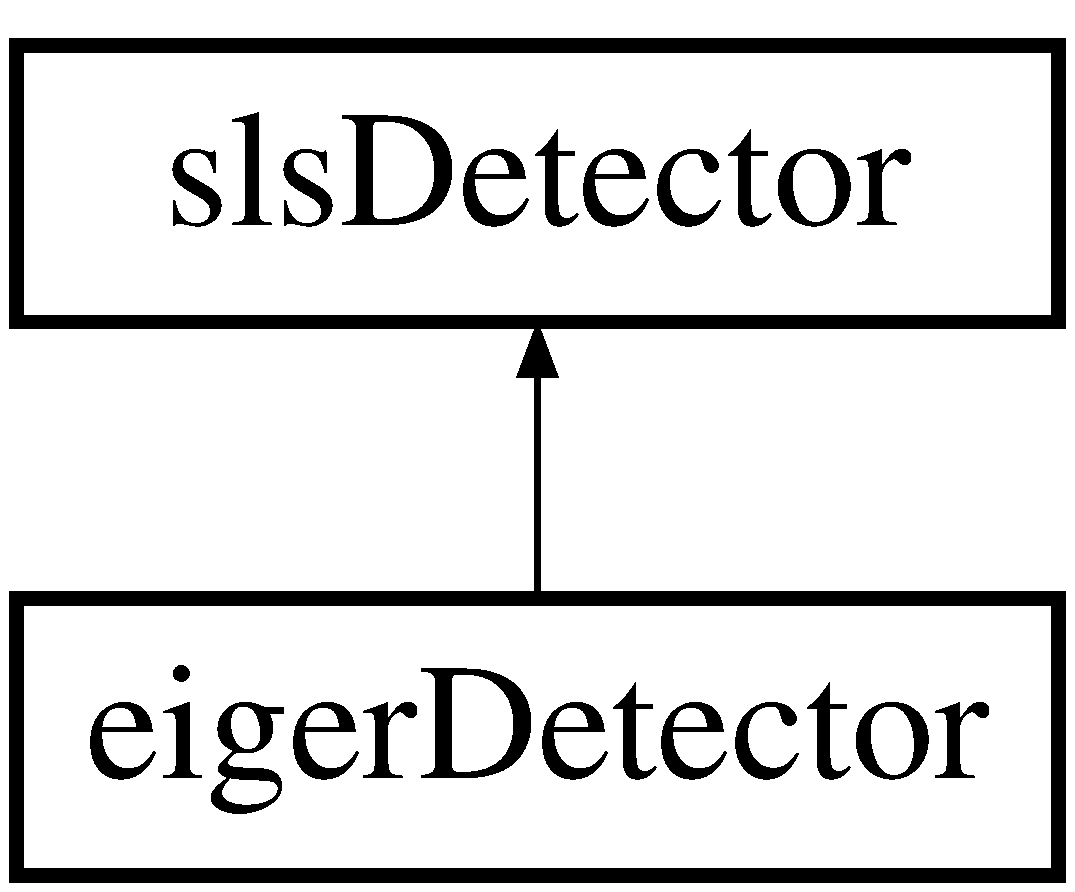
\includegraphics[height=2cm]{classeigerDetector}
\end{center}
\end{figure}
\subsection*{Public Member Functions}
\begin{CompactItemize}
\item 
\bf{eiger\-Detector} (int id=0)
\item 
\bf{$\sim$eiger\-Detector} ()
\item 
\bf{sls\_\-detector\_\-module} $\ast$ \bf{read\-Trim\-File} (string fname, \bf{sls\_\-detector\_\-module} $\ast$my\-Mod=NULL)
\item 
int \bf{write\-Trim\-File} (string fname, \bf{sls\_\-detector\_\-module} mod)
\item 
int \bf{write\-Trim\-File} (string fname, int imod)
\item 
int \bf{write\-Data\-File} (string fname, float $\ast$data, float $\ast$err=NULL, float $\ast$ang=NULL, char dataformat='f', int nch=-1)
\item 
int \bf{write\-Data\-File} (string fname, int $\ast$data)
\item 
int \bf{read\-Data\-File} (string fname, float $\ast$data, float $\ast$err=NULL, float $\ast$ang=NULL, char dataformat='f', int nch=0)
\item 
int \bf{read\-Data\-File} (string fname, int $\ast$data)
\item 
int \bf{read\-Calibration\-File} (string fname, float \&gain, float \&offset)
\item 
int \bf{write\-Calibration\-File} (string fname, float gain, float offset)
\item 
float $\ast$ \bf{decode\-Data} (int $\ast$datain)
\end{CompactItemize}


\subsection{Detailed Description}
This is class contains all eiger specific functionalities. 

The \doxyref{mythen\-Detector}{p.}{classmythenDetector} class contains the functions specific to the eiger detector

\begin{Desc}
\item[Author:]Anna Bergamaschi \end{Desc}
\begin{Desc}
\item[Version:]0.1alpha (any string) \end{Desc}




\subsection{Constructor \& Destructor Documentation}
\index{eigerDetector@{eiger\-Detector}!eigerDetector@{eigerDetector}}
\index{eigerDetector@{eigerDetector}!eigerDetector@{eiger\-Detector}}
\subsubsection{\setlength{\rightskip}{0pt plus 5cm}eiger\-Detector::eiger\-Detector (int {\em id} = {\tt 0})}\label{classeigerDetector_591261cd5af00795657b44ee2681ced3}


(default) constructor

\begin{Desc}
\item[Parameters:]
\begin{description}
\item[{\em id}]is the detector index which is needed to define the shared memory id. Different physical detectors should have different IDs in order to work independently \end{description}
\end{Desc}
\index{eigerDetector@{eiger\-Detector}!~eigerDetector@{$\sim$eigerDetector}}
\index{~eigerDetector@{$\sim$eigerDetector}!eigerDetector@{eiger\-Detector}}
\subsubsection{\setlength{\rightskip}{0pt plus 5cm}eiger\-Detector::$\sim$eiger\-Detector ()\hspace{0.3cm}{\tt  [inline]}}\label{classeigerDetector_aa968c7588fb7200a8764a08196ac549}


destructor 

\subsection{Member Function Documentation}
\index{eigerDetector@{eiger\-Detector}!decodeData@{decodeData}}
\index{decodeData@{decodeData}!eigerDetector@{eiger\-Detector}}
\subsubsection{\setlength{\rightskip}{0pt plus 5cm}float$\ast$ eiger\-Detector::decode\-Data (int $\ast$ {\em datain})}\label{classeigerDetector_3e0573baf38c37818c7769fb351010b3}


decode data from the detector converting them to an array of floats, one for each channle \begin{Desc}
\item[Parameters:]
\begin{description}
\item[{\em datain}]data from the detector \end{description}
\end{Desc}
\begin{Desc}
\item[Returns:]pointer to a float array with a data per channel \end{Desc}


Reimplemented from \bf{sls\-Detector} \doxyref{p.}{classslsDetector_937d257464bade6dc6d3ab42c86843ba}.\index{eigerDetector@{eiger\-Detector}!readCalibrationFile@{readCalibrationFile}}
\index{readCalibrationFile@{readCalibrationFile}!eigerDetector@{eiger\-Detector}}
\subsubsection{\setlength{\rightskip}{0pt plus 5cm}int eiger\-Detector::read\-Calibration\-File (string {\em fname}, float \& {\em gain}, float \& {\em offset})\hspace{0.3cm}{\tt  [virtual]}}\label{classeigerDetector_6b1b4b5328a5d8c423e9a7a8a950028f}


int \doxyref{read\-Calibration\-File(string fname, float \&gain, float \&offset)}{p.}{classeigerDetector_6b1b4b5328a5d8c423e9a7a8a950028f};

\begin{Desc}
\item[Parameters:]
\begin{description}
\item[{\em fname}]file to be read \item[{\em gain}]reference to the gain variable  reference to the offset variable \end{description}
\end{Desc}
\begin{Desc}
\item[See also:]\doxyref{shared\-Sls\-Detector}{p.}{classslsDetector_2dd6bff7d94ab8005c2797152b19264e} \end{Desc}


Implements \bf{sls\-Detector} \doxyref{p.}{classslsDetector_6c7f837f0820b08f41649c30151cb7ac}.\index{eigerDetector@{eiger\-Detector}!readDataFile@{readDataFile}}
\index{readDataFile@{readDataFile}!eigerDetector@{eiger\-Detector}}
\subsubsection{\setlength{\rightskip}{0pt plus 5cm}int eiger\-Detector::read\-Data\-File (string {\em fname}, int $\ast$ {\em data})\hspace{0.3cm}{\tt  [virtual]}}\label{classeigerDetector_a6afa206101506d7f95d1ec835fbf843}


reads a data file \begin{Desc}
\item[Parameters:]
\begin{description}
\item[{\em name}]of the file to be read \item[{\em data}]array of data values \end{description}
\end{Desc}
\begin{Desc}
\item[Returns:]OK or FAIL if it could not read the file or data=NULL \end{Desc}


Implements \bf{sls\-Detector} \doxyref{p.}{classslsDetector_4239e7a357df82640464c0f2d0a18d69}.\index{eigerDetector@{eiger\-Detector}!readDataFile@{readDataFile}}
\index{readDataFile@{readDataFile}!eigerDetector@{eiger\-Detector}}
\subsubsection{\setlength{\rightskip}{0pt plus 5cm}int eiger\-Detector::read\-Data\-File (string {\em fname}, float $\ast$ {\em data}, float $\ast$ {\em err} = {\tt NULL}, float $\ast$ {\em ang} = {\tt NULL}, char {\em dataformat} = {\tt 'f'}, int {\em nch} = {\tt 0})\hspace{0.3cm}{\tt  [virtual]}}\label{classeigerDetector_4d0b7da609b9a0457656bfc8cf0a7997}


reads a data file \begin{Desc}
\item[Parameters:]
\begin{description}
\item[{\em name}]of the file to be read \item[{\em data}]array of data values to be filled \item[{\em err}]array of arrors on the data. If NULL no errors are expected on the file\item[{\em ang}]array of angular values. If NULL data are expected in the form chan-val(-err) otherwise ang-val(-err) \item[{\em dataformat}]format of the data: can be 'i' integer or 'f' float (default) \item[{\em nch}]number of channels to be written to file. if $<$=0 defaults to the number of installed channels of the detector \end{description}
\end{Desc}
\begin{Desc}
\item[Returns:]OK or FAIL if it could not read the file or data=NULL \end{Desc}


Implements \bf{sls\-Detector} \doxyref{p.}{classslsDetector_86df95809e0e7979eafc04b2b868843d}.\index{eigerDetector@{eiger\-Detector}!readTrimFile@{readTrimFile}}
\index{readTrimFile@{readTrimFile}!eigerDetector@{eiger\-Detector}}
\subsubsection{\setlength{\rightskip}{0pt plus 5cm}\bf{sls\_\-detector\_\-module}$\ast$ eiger\-Detector::read\-Trim\-File (string {\em fname}, \bf{sls\_\-detector\_\-module} $\ast$ {\em my\-Mod} = {\tt NULL})\hspace{0.3cm}{\tt  [virtual]}}\label{classeigerDetector_f24af0459e8eb45c1bc9c68a870e5094}


reads a trim file \begin{Desc}
\item[Parameters:]
\begin{description}
\item[{\em fname}]name of the file to be read \item[{\em my\-Mod}]pointer to the module structure which has to be set. \par
 If it is NULL a new module structure will be created \end{description}
\end{Desc}
\begin{Desc}
\item[Returns:]the pointer to my\-Mod or NULL if reading the file failed \end{Desc}


Implements \bf{sls\-Detector} \doxyref{p.}{classslsDetector_612b52469e27c6675969499d3680abe6}.\index{eigerDetector@{eiger\-Detector}!writeCalibrationFile@{writeCalibrationFile}}
\index{writeCalibrationFile@{writeCalibrationFile}!eigerDetector@{eiger\-Detector}}
\subsubsection{\setlength{\rightskip}{0pt plus 5cm}int eiger\-Detector::write\-Calibration\-File (string {\em fname}, float {\em gain}, float {\em offset})\hspace{0.3cm}{\tt  [virtual]}}\label{classeigerDetector_d5fbecfcc46cb151160c6011aa8e33b2}


writes a clibration file \begin{Desc}
\item[Parameters:]
\begin{description}
\item[{\em fname}]file to be written \item[{\em gain}]\item[{\em offset}]\end{description}
\end{Desc}
\begin{Desc}
\item[See also:]\doxyref{shared\-Sls\-Detector}{p.}{classslsDetector_2dd6bff7d94ab8005c2797152b19264e} \end{Desc}


Implements \bf{sls\-Detector} \doxyref{p.}{classslsDetector_d12edef440bf2b2f930e83f0ccceb01e}.\index{eigerDetector@{eiger\-Detector}!writeDataFile@{writeDataFile}}
\index{writeDataFile@{writeDataFile}!eigerDetector@{eiger\-Detector}}
\subsubsection{\setlength{\rightskip}{0pt plus 5cm}int eiger\-Detector::write\-Data\-File (string {\em fname}, int $\ast$ {\em data})\hspace{0.3cm}{\tt  [virtual]}}\label{classeigerDetector_68a740d5e43fcdb00c57f401666c0856}


writes a data file \begin{Desc}
\item[Parameters:]
\begin{description}
\item[{\em name}]of the file to be written \item[{\em data}]array of data values \end{description}
\end{Desc}
\begin{Desc}
\item[Returns:]OK or FAIL if it could not write the file or data=NULL \end{Desc}


Implements \bf{sls\-Detector} \doxyref{p.}{classslsDetector_efa98ca652306e2a026c9a5b2fbfe2dc}.\index{eigerDetector@{eiger\-Detector}!writeDataFile@{writeDataFile}}
\index{writeDataFile@{writeDataFile}!eigerDetector@{eiger\-Detector}}
\subsubsection{\setlength{\rightskip}{0pt plus 5cm}int eiger\-Detector::write\-Data\-File (string {\em fname}, float $\ast$ {\em data}, float $\ast$ {\em err} = {\tt NULL}, float $\ast$ {\em ang} = {\tt NULL}, char {\em dataformat} = {\tt 'f'}, int {\em nch} = {\tt -1})\hspace{0.3cm}{\tt  [virtual]}}\label{classeigerDetector_5ad2bf5b10d17e8c4ad7ae6e81e647e0}


writes a data file \begin{Desc}
\item[Parameters:]
\begin{description}
\item[{\em name}]of the file to be written \item[{\em data}]array of data values \item[{\em err}]array of arrors on the data. If NULL no errors will be written\item[{\em ang}]array of angular values. If NULL data will be in the form chan-val(-err) otherwise ang-val(-err) \item[{\em dataformat}]format of the data: can be 'i' integer or 'f' float (default) \item[{\em nch}]number of channels to be written to file. if -1 defaults to the number of installed channels of the detector \end{description}
\end{Desc}
\begin{Desc}
\item[Returns:]OK or FAIL if it could not write the file or data=NULL \end{Desc}


Implements \bf{sls\-Detector} \doxyref{p.}{classslsDetector_08823d7078b5e6dd1a4cb7d8b3cfe0af}.\index{eigerDetector@{eiger\-Detector}!writeTrimFile@{writeTrimFile}}
\index{writeTrimFile@{writeTrimFile}!eigerDetector@{eiger\-Detector}}
\subsubsection{\setlength{\rightskip}{0pt plus 5cm}int eiger\-Detector::write\-Trim\-File (string {\em fname}, int {\em imod})\hspace{0.3cm}{\tt  [virtual]}}\label{classeigerDetector_df3a0dff0fc3111e10af0363bdd15a6a}


writes a trim file for module number imod - the values will be read from the current detector structure \begin{Desc}
\item[Parameters:]
\begin{description}
\item[{\em fname}]name of the file to be written \item[{\em imod}]module number \end{description}
\end{Desc}
\begin{Desc}
\item[Returns:]OK or FAIL if the file could not be written \end{Desc}
\begin{Desc}
\item[See also:]\doxyref{sls\_\-detector\_\-module}{p.}{structsls__detector__module} \doxyref{shared\-Sls\-Detector}{p.}{classslsDetector_2dd6bff7d94ab8005c2797152b19264e} \end{Desc}


Implements \bf{sls\-Detector} \doxyref{p.}{classslsDetector_cb27a987551e66093eb201523ac8d8b0}.\index{eigerDetector@{eiger\-Detector}!writeTrimFile@{writeTrimFile}}
\index{writeTrimFile@{writeTrimFile}!eigerDetector@{eiger\-Detector}}
\subsubsection{\setlength{\rightskip}{0pt plus 5cm}int eiger\-Detector::write\-Trim\-File (string {\em fname}, \bf{sls\_\-detector\_\-module} {\em mod})\hspace{0.3cm}{\tt  [virtual]}}\label{classeigerDetector_8380366bf7112021c49be8e6f29f18d8}


writes a trim file \begin{Desc}
\item[Parameters:]
\begin{description}
\item[{\em fname}]name of the file to be written \item[{\em mod}]module structure which has to be written to file \end{description}
\end{Desc}
\begin{Desc}
\item[Returns:]OK or FAIL if the file could not be written\end{Desc}
\begin{Desc}
\item[See also:]\doxyref{sls\_\-detector\_\-module}{p.}{structsls__detector__module} \end{Desc}


Implements \bf{sls\-Detector} \doxyref{p.}{classslsDetector_5b97351cfaffe067016dbcebbd0778a7}.

The documentation for this class was generated from the following file:\begin{CompactItemize}
\item 
eiger\-Detector/\bf{eiger\-Detector.h}\end{CompactItemize}

\section{iarray Struct Reference}
\label{structiarray}\index{iarray@{iarray}}
{\tt \#include $<$sls\_\-detector\_\-defs.h$>$}

\subsection*{Public Attributes}
\begin{CompactItemize}
\item 
int \bf{len}
\item 
int $\ast$ \bf{iptr}
\end{CompactItemize}


\subsection{Detailed Description}
structure for a generic integer array 



\subsection{Member Data Documentation}
\index{iarray@{iarray}!iptr@{iptr}}
\index{iptr@{iptr}!iarray@{iarray}}
\subsubsection{\setlength{\rightskip}{0pt plus 5cm}int$\ast$ \bf{iarray::iptr}}\label{structiarray_65e4e79e4c42d1d3b075d84bff7046c4}


is the pointer to the array \index{iarray@{iarray}!len@{len}}
\index{len@{len}!iarray@{iarray}}
\subsubsection{\setlength{\rightskip}{0pt plus 5cm}int \bf{iarray::len}}\label{structiarray_97fedf6b925f79b2883d07300b266869}


is the number of elements of the array 

The documentation for this struct was generated from the following file:\begin{CompactItemize}
\item 
common\-Files/\bf{sls\_\-detector\_\-defs.h}\end{CompactItemize}

\section{My\-Socket\-TCP Class Reference}
\label{classMySocketTCP}\index{MySocketTCP@{MySocketTCP}}
{\tt \#include $<$My\-Socket\-TCP.h$>$}

\subsection*{Public Member Functions}
\begin{CompactItemize}
\item 
\bf{My\-Socket\-TCP} (const char $\ast$const host\_\-ip\_\-or\_\-name, unsigned short int const port\_\-number)
\item 
\bf{My\-Socket\-TCP} (unsigned short int const port\_\-number)
\item 
\bf{$\sim$My\-Socket\-TCP} ()
\item 
int \bf{get\-Hostname} (char $\ast$name)
\item 
int \bf{get\-Port\-Number} ()
\item 
int \bf{get\-Error\-Status} ()
\item 
int \bf{Connect} ()
\item 
void \bf{Disconnect} ()
\item 
int \bf{Send\-Data} (void $\ast$buf, int length)
\item 
int \bf{Receive\-Data} (void $\ast$buf, int length)
\item 
int \bf{Send\-Data\-And\-Keep\-Connection} (void $\ast$buf, int length)
\item 
int \bf{Receive\-Data\-And\-Keep\-Connection} (void $\ast$buf, int length)
\item 
int \bf{Send\-Data\-Only} (void $\ast$buf, int length)
\item 
int \bf{Receive\-Data\-Only} (void $\ast$buf, int length)
\end{CompactItemize}
\subsection*{Private Attributes}
\begin{CompactItemize}
\item 
char \bf{hostname} [1000]
\item 
int \bf{portno}
\item 
int \bf{is\_\-a\_\-server}
\item 
int \bf{socket\-Descriptor}
\item 
sockaddr\_\-in client\-Address \bf{server\-Address}
\item 
socklen\_\-t \bf{client\-Address\_\-length}
\item 
int \bf{file\_\-des}
\item 
int \bf{send\_\-rec\_\-max\_\-size}
\item 
bool \bf{last\_\-keep\_\-connection\_\-open\_\-action\_\-was\_\-a\_\-send}
\end{CompactItemize}


\subsection{Constructor \& Destructor Documentation}
\index{MySocketTCP@{My\-Socket\-TCP}!MySocketTCP@{MySocketTCP}}
\index{MySocketTCP@{MySocketTCP}!MySocketTCP@{My\-Socket\-TCP}}
\subsubsection{\setlength{\rightskip}{0pt plus 5cm}My\-Socket\-TCP::My\-Socket\-TCP (const char $\ast$const  {\em host\_\-ip\_\-or\_\-name}, unsigned short int const  {\em port\_\-number})}\label{classMySocketTCP_4d44c3d3d93c2990bcdff6a58016a170}


\index{MySocketTCP@{My\-Socket\-TCP}!MySocketTCP@{MySocketTCP}}
\index{MySocketTCP@{MySocketTCP}!MySocketTCP@{My\-Socket\-TCP}}
\subsubsection{\setlength{\rightskip}{0pt plus 5cm}My\-Socket\-TCP::My\-Socket\-TCP (unsigned short int const  {\em port\_\-number})}\label{classMySocketTCP_1033d3d7438fe9da3cff3da3c4344c51}


\index{MySocketTCP@{My\-Socket\-TCP}!~MySocketTCP@{$\sim$MySocketTCP}}
\index{~MySocketTCP@{$\sim$MySocketTCP}!MySocketTCP@{My\-Socket\-TCP}}
\subsubsection{\setlength{\rightskip}{0pt plus 5cm}My\-Socket\-TCP::$\sim$My\-Socket\-TCP ()}\label{classMySocketTCP_20407e0c509b8e32e164f1780b98b51c}




\subsection{Member Function Documentation}
\index{MySocketTCP@{My\-Socket\-TCP}!Connect@{Connect}}
\index{Connect@{Connect}!MySocketTCP@{My\-Socket\-TCP}}
\subsubsection{\setlength{\rightskip}{0pt plus 5cm}int My\-Socket\-TCP::Connect ()}\label{classMySocketTCP_1debe73787357c6dcec52ca981298609}


\index{MySocketTCP@{My\-Socket\-TCP}!Disconnect@{Disconnect}}
\index{Disconnect@{Disconnect}!MySocketTCP@{My\-Socket\-TCP}}
\subsubsection{\setlength{\rightskip}{0pt plus 5cm}void My\-Socket\-TCP::Disconnect ()}\label{classMySocketTCP_69f0b72663378245f14e2872b92696a4}


\index{MySocketTCP@{My\-Socket\-TCP}!getErrorStatus@{getErrorStatus}}
\index{getErrorStatus@{getErrorStatus}!MySocketTCP@{My\-Socket\-TCP}}
\subsubsection{\setlength{\rightskip}{0pt plus 5cm}int My\-Socket\-TCP::get\-Error\-Status ()\hspace{0.3cm}{\tt  [inline]}}\label{classMySocketTCP_8cd662e945f4a51e9f616fd5c196bdeb}


\index{MySocketTCP@{My\-Socket\-TCP}!getHostname@{getHostname}}
\index{getHostname@{getHostname}!MySocketTCP@{My\-Socket\-TCP}}
\subsubsection{\setlength{\rightskip}{0pt plus 5cm}int My\-Socket\-TCP::get\-Hostname (char $\ast$ {\em name})}\label{classMySocketTCP_6c3f62f34cf58c78d58bcc788776afa5}


\index{MySocketTCP@{My\-Socket\-TCP}!getPortNumber@{getPortNumber}}
\index{getPortNumber@{getPortNumber}!MySocketTCP@{My\-Socket\-TCP}}
\subsubsection{\setlength{\rightskip}{0pt plus 5cm}int My\-Socket\-TCP::get\-Port\-Number ()\hspace{0.3cm}{\tt  [inline]}}\label{classMySocketTCP_8d15a71679ab2f83822db875be1ad5cd}


\index{MySocketTCP@{My\-Socket\-TCP}!ReceiveData@{ReceiveData}}
\index{ReceiveData@{ReceiveData}!MySocketTCP@{My\-Socket\-TCP}}
\subsubsection{\setlength{\rightskip}{0pt plus 5cm}int My\-Socket\-TCP::Receive\-Data (void $\ast$ {\em buf}, int {\em length})}\label{classMySocketTCP_ed8a6a9435932659ed8793ff57b356c8}


\index{MySocketTCP@{My\-Socket\-TCP}!ReceiveDataAndKeepConnection@{ReceiveDataAndKeepConnection}}
\index{ReceiveDataAndKeepConnection@{ReceiveDataAndKeepConnection}!MySocketTCP@{My\-Socket\-TCP}}
\subsubsection{\setlength{\rightskip}{0pt plus 5cm}int My\-Socket\-TCP::Receive\-Data\-And\-Keep\-Connection (void $\ast$ {\em buf}, int {\em length})}\label{classMySocketTCP_375171791400d7d60804b56852ff3611}


\index{MySocketTCP@{My\-Socket\-TCP}!ReceiveDataOnly@{ReceiveDataOnly}}
\index{ReceiveDataOnly@{ReceiveDataOnly}!MySocketTCP@{My\-Socket\-TCP}}
\subsubsection{\setlength{\rightskip}{0pt plus 5cm}int My\-Socket\-TCP::Receive\-Data\-Only (void $\ast$ {\em buf}, int {\em length})}\label{classMySocketTCP_a8b6322845e72ffc6da44db774b19d73}


\index{MySocketTCP@{My\-Socket\-TCP}!SendData@{SendData}}
\index{SendData@{SendData}!MySocketTCP@{My\-Socket\-TCP}}
\subsubsection{\setlength{\rightskip}{0pt plus 5cm}int My\-Socket\-TCP::Send\-Data (void $\ast$ {\em buf}, int {\em length})}\label{classMySocketTCP_7777e909e20c47d38e32a174b0eae425}


\index{MySocketTCP@{My\-Socket\-TCP}!SendDataAndKeepConnection@{SendDataAndKeepConnection}}
\index{SendDataAndKeepConnection@{SendDataAndKeepConnection}!MySocketTCP@{My\-Socket\-TCP}}
\subsubsection{\setlength{\rightskip}{0pt plus 5cm}int My\-Socket\-TCP::Send\-Data\-And\-Keep\-Connection (void $\ast$ {\em buf}, int {\em length})}\label{classMySocketTCP_1641bc23538af6849efeb195a1b33626}


\index{MySocketTCP@{My\-Socket\-TCP}!SendDataOnly@{SendDataOnly}}
\index{SendDataOnly@{SendDataOnly}!MySocketTCP@{My\-Socket\-TCP}}
\subsubsection{\setlength{\rightskip}{0pt plus 5cm}int My\-Socket\-TCP::Send\-Data\-Only (void $\ast$ {\em buf}, int {\em length})}\label{classMySocketTCP_2f9ce7233ee4903127039d43b4a34886}




\subsection{Member Data Documentation}
\index{MySocketTCP@{My\-Socket\-TCP}!clientAddress_length@{clientAddress\_\-length}}
\index{clientAddress_length@{clientAddress\_\-length}!MySocketTCP@{My\-Socket\-TCP}}
\subsubsection{\setlength{\rightskip}{0pt plus 5cm}socklen\_\-t \bf{My\-Socket\-TCP::client\-Address\_\-length}\hspace{0.3cm}{\tt  [private]}}\label{classMySocketTCP_446008276e7be89c50bd78f9a3015a69}


\index{MySocketTCP@{My\-Socket\-TCP}!file_des@{file\_\-des}}
\index{file_des@{file\_\-des}!MySocketTCP@{My\-Socket\-TCP}}
\subsubsection{\setlength{\rightskip}{0pt plus 5cm}int \bf{My\-Socket\-TCP::file\_\-des}\hspace{0.3cm}{\tt  [private]}}\label{classMySocketTCP_8a6787a3cdb6b4539184b92303958f30}


\index{MySocketTCP@{My\-Socket\-TCP}!hostname@{hostname}}
\index{hostname@{hostname}!MySocketTCP@{My\-Socket\-TCP}}
\subsubsection{\setlength{\rightskip}{0pt plus 5cm}char \bf{My\-Socket\-TCP::hostname}[1000]\hspace{0.3cm}{\tt  [private]}}\label{classMySocketTCP_bfd6f681b235f233d3203336a89d58f2}


\index{MySocketTCP@{My\-Socket\-TCP}!is_a_server@{is\_\-a\_\-server}}
\index{is_a_server@{is\_\-a\_\-server}!MySocketTCP@{My\-Socket\-TCP}}
\subsubsection{\setlength{\rightskip}{0pt plus 5cm}int \bf{My\-Socket\-TCP::is\_\-a\_\-server}\hspace{0.3cm}{\tt  [private]}}\label{classMySocketTCP_e95406b86fb4f0e1978c49f0ac9d3821}


\index{MySocketTCP@{My\-Socket\-TCP}!last_keep_connection_open_action_was_a_send@{last\_\-keep\_\-connection\_\-open\_\-action\_\-was\_\-a\_\-send}}
\index{last_keep_connection_open_action_was_a_send@{last\_\-keep\_\-connection\_\-open\_\-action\_\-was\_\-a\_\-send}!MySocketTCP@{My\-Socket\-TCP}}
\subsubsection{\setlength{\rightskip}{0pt plus 5cm}bool \bf{My\-Socket\-TCP::last\_\-keep\_\-connection\_\-open\_\-action\_\-was\_\-a\_\-send}\hspace{0.3cm}{\tt  [private]}}\label{classMySocketTCP_e0cdfa6a0f0498c01d057ff5db10dca5}


\index{MySocketTCP@{My\-Socket\-TCP}!portno@{portno}}
\index{portno@{portno}!MySocketTCP@{My\-Socket\-TCP}}
\subsubsection{\setlength{\rightskip}{0pt plus 5cm}int \bf{My\-Socket\-TCP::portno}\hspace{0.3cm}{\tt  [private]}}\label{classMySocketTCP_cc9182c599b55d4f081c31cb162d56f6}


\index{MySocketTCP@{My\-Socket\-TCP}!send_rec_max_size@{send\_\-rec\_\-max\_\-size}}
\index{send_rec_max_size@{send\_\-rec\_\-max\_\-size}!MySocketTCP@{My\-Socket\-TCP}}
\subsubsection{\setlength{\rightskip}{0pt plus 5cm}int \bf{My\-Socket\-TCP::send\_\-rec\_\-max\_\-size}\hspace{0.3cm}{\tt  [private]}}\label{classMySocketTCP_702056a78e403d4931181d54e7263290}


\index{MySocketTCP@{My\-Socket\-TCP}!serverAddress@{serverAddress}}
\index{serverAddress@{serverAddress}!MySocketTCP@{My\-Socket\-TCP}}
\subsubsection{\setlength{\rightskip}{0pt plus 5cm}struct sockaddr\_\-in client\-Address \bf{My\-Socket\-TCP::server\-Address}\hspace{0.3cm}{\tt  [private]}}\label{classMySocketTCP_02c455c28f7aff0075c954c43715dad2}


\index{MySocketTCP@{My\-Socket\-TCP}!socketDescriptor@{socketDescriptor}}
\index{socketDescriptor@{socketDescriptor}!MySocketTCP@{My\-Socket\-TCP}}
\subsubsection{\setlength{\rightskip}{0pt plus 5cm}int \bf{My\-Socket\-TCP::socket\-Descriptor}\hspace{0.3cm}{\tt  [private]}}\label{classMySocketTCP_7246bd46ad899956f39109e528da0567}




The documentation for this class was generated from the following files:\begin{CompactItemize}
\item 
My\-Socket\-TCP/\bf{My\-Socket\-TCP.h}\item 
My\-Socket\-TCP/\bf{My\-Socket\-TCP.cxx}\end{CompactItemize}

\section{mythen\-Detector Class Reference}
\label{classmythenDetector}\index{mythenDetector@{mythenDetector}}
{\tt \#include $<$mythen\-Detector.h$>$}

Inheritance diagram for mythen\-Detector::\begin{figure}[H]
\begin{center}
\leavevmode
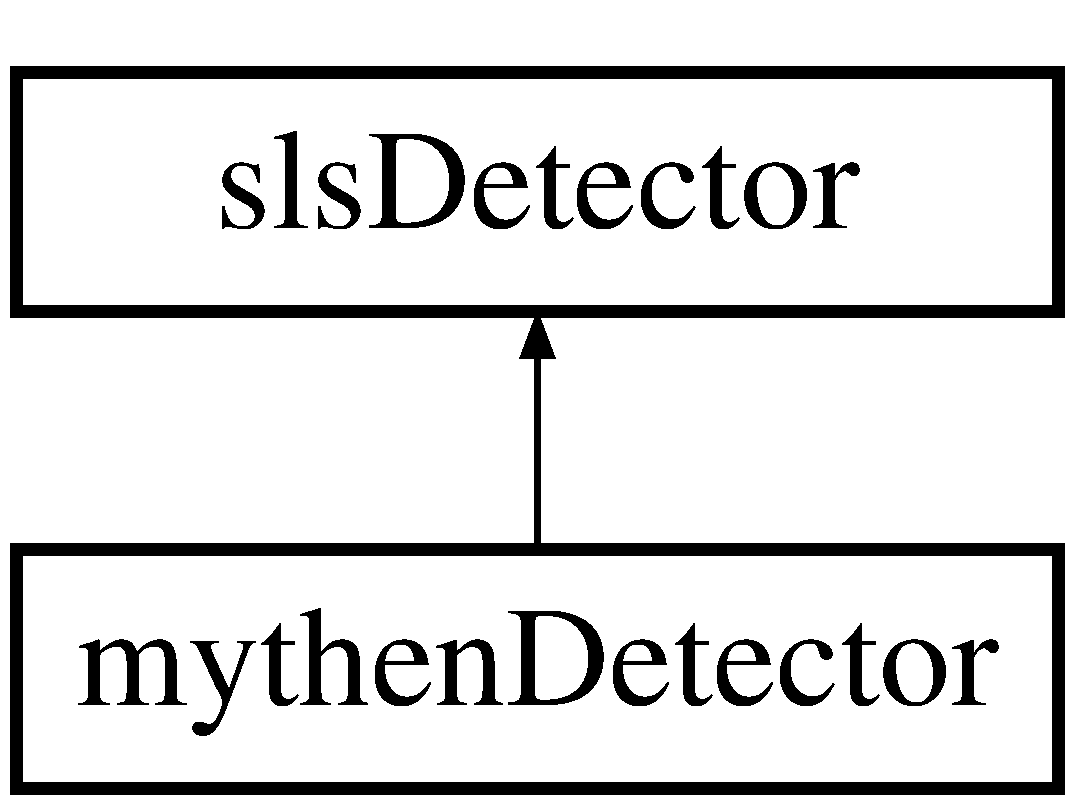
\includegraphics[height=2cm]{classmythenDetector}
\end{center}
\end{figure}
\subsection*{Public Member Functions}
\begin{CompactItemize}
\item 
\bf{mythen\-Detector} (int id=0)
\item 
\bf{$\sim$mythen\-Detector} ()
\item 
int \bf{read\-Configuration\-File} (string const fname)
\item 
int \bf{write\-Configuration\-File} (string const fname)
\item 
int \bf{dump\-Detector\-Setup} (string const fname)
\item 
int \bf{retrieve\-Detector\-Setup} (string const fname)
\item 
\bf{sls\_\-detector\_\-module} $\ast$ \bf{read\-Trim\-File} (string fname, \bf{sls\_\-detector\_\-module} $\ast$my\-Mod=NULL)
\item 
int \bf{write\-Trim\-File} (string fname, \bf{sls\_\-detector\_\-module} mod)
\item 
int \bf{write\-Trim\-File} (string fname, int imod)
\item 
int \bf{write\-Data\-File} (string fname, float $\ast$data, float $\ast$err=NULL, float $\ast$ang=NULL, char dataformat='f', int nch=-1)
\item 
int \bf{write\-Data\-File} (string fname, int $\ast$data)
\item 
int \bf{read\-Data\-File} (string fname, float $\ast$data, float $\ast$err=NULL, float $\ast$ang=NULL, char dataformat='f', int nch=0)
\item 
int \bf{read\-Data\-File} (string fname, int $\ast$data)
\item 
int \bf{read\-Calibration\-File} (string fname, float \&gain, float \&offset)
\item 
int \bf{write\-Calibration\-File} (string fname, float gain, float offset)
\item 
int \bf{read\-Angular\-Conversion} (string fname=\char`\"{}\char`\"{})
\item 
int \bf{write\-Angular\-Conversion} (string fname=\char`\"{}\char`\"{})
\item 
int \bf{set\-Angular\-Conversion} (string fname=\char`\"{}\char`\"{})
\item 
int \bf{get\-Angular\-Conversion} (int \&direction, \bf{angle\-Conversion\-Constant} $\ast$angconv=NULL)
\item 
char $\ast$ \bf{get\-Angular\-Conversion} ()
\item 
float \bf{set\-Global\-Offset} (float f)
\item 
float \bf{set\-Fine\-Offset} (float f)
\item 
float \bf{get\-Fine\-Offset} ()
\item 
float \bf{get\-Global\-Offset} ()
\item 
int \bf{set\-Positions} (int n\-Pos, float $\ast$\bf{pos})
\item 
int \bf{get\-Positions} (float $\ast$\bf{pos}=NULL)
\item 
float \bf{set\-Bin\-Size} (float bs)
\item 
float \bf{get\-Bin\-Size} ()
\item 
int \bf{reset\-Merging} (float $\ast$mp, float $\ast$mv, float $\ast$me, int $\ast$mm)
\item 
int \bf{add\-To\-Merging} (float $\ast$p1, float $\ast$v1, float $\ast$e1, float $\ast$mp, float $\ast$mv, float $\ast$me, int $\ast$mm)
\item 
int \bf{finalize\-Merging} (float $\ast$mp, float $\ast$mv, float $\ast$me, int $\ast$mm)
\item 
void $\ast$ \bf{process\-Data} (int delflag=1)
\item 
void \bf{acquire} (int delflag=1)
\end{CompactItemize}


\subsection{Constructor \& Destructor Documentation}
\index{mythenDetector@{mythen\-Detector}!mythenDetector@{mythenDetector}}
\index{mythenDetector@{mythenDetector}!mythenDetector@{mythen\-Detector}}
\subsubsection{\setlength{\rightskip}{0pt plus 5cm}mythen\-Detector::mythen\-Detector (int {\em id} = {\tt 0})\hspace{0.3cm}{\tt  [inline]}}\label{classmythenDetector_5efa6a91622e5e173d7491801f60bda0}


(default) constructor \index{mythenDetector@{mythen\-Detector}!~mythenDetector@{$\sim$mythenDetector}}
\index{~mythenDetector@{$\sim$mythenDetector}!mythenDetector@{mythen\-Detector}}
\subsubsection{\setlength{\rightskip}{0pt plus 5cm}mythen\-Detector::$\sim$mythen\-Detector ()\hspace{0.3cm}{\tt  [inline]}}\label{classmythenDetector_8118166c2e7c3d3968b9ae5016614693}


destructor 

\subsection{Member Function Documentation}
\index{mythenDetector@{mythen\-Detector}!acquire@{acquire}}
\index{acquire@{acquire}!mythenDetector@{mythen\-Detector}}
\subsubsection{\setlength{\rightskip}{0pt plus 5cm}void mythen\-Detector::acquire (int {\em delflag} = {\tt 1})\hspace{0.3cm}{\tt  [virtual]}}\label{classmythenDetector_f393765b5a3d5f8f05251116f38d52dd}


performs the complete acquisition and data processing moves the detector to next position \par
 starts and reads the detector \par
 reads the IC (if required) \par
 reads the encoder (iof required for angualr conversion) \par
 processes the data (flat field, rate, angular conversion and merging process\-Data()) \begin{Desc}
\item[Parameters:]
\begin{description}
\item[{\em delflag}]if 1 the data are deleted, else left there for further processing (or plotting?) \end{description}
\end{Desc}


Implements \bf{sls\-Detector} \doxyref{p.}{classslsDetector_1af6548fd0d81d45909a5c805d4be7a8}.\index{mythenDetector@{mythen\-Detector}!addToMerging@{addToMerging}}
\index{addToMerging@{addToMerging}!mythenDetector@{mythen\-Detector}}
\subsubsection{\setlength{\rightskip}{0pt plus 5cm}int mythen\-Detector::add\-To\-Merging (float $\ast$ {\em p1}, float $\ast$ {\em v1}, float $\ast$ {\em e1}, float $\ast$ {\em mp}, float $\ast$ {\em mv}, float $\ast$ {\em me}, int $\ast$ {\em mm})\hspace{0.3cm}{\tt  [virtual]}}\label{classmythenDetector_eaaf7d7e3150f473e3bbcf59d91692c2}


merge dataset \begin{Desc}
\item[Parameters:]
\begin{description}
\item[{\em p1}]angular positions of dataset \item[{\em v1}]data \item[{\em e1}]errors \item[{\em mp}]already merged postions \item[{\em mv}]already merged data \item[{\em me}]already merged errors (squared sum) \item[{\em mm}]multiplicity of merged arrays \end{description}
\end{Desc}


Implements \bf{sls\-Detector} \doxyref{p.}{classslsDetector_feb8730f24292620e5d451cd2d4bb9cd}.\index{mythenDetector@{mythen\-Detector}!dumpDetectorSetup@{dumpDetectorSetup}}
\index{dumpDetectorSetup@{dumpDetectorSetup}!mythenDetector@{mythen\-Detector}}
\subsubsection{\setlength{\rightskip}{0pt plus 5cm}int mythen\-Detector::dump\-Detector\-Setup (string const  {\em fname})\hspace{0.3cm}{\tt  [virtual]}}\label{classmythenDetector_a0fe9987e8fa240a312ad353ae539188}


not yet implemented

should dump to a file all the current detector parameters 

Implements \bf{sls\-Detector} \doxyref{p.}{classslsDetector_96428855d6e286408a52e675e045cf45}.\index{mythenDetector@{mythen\-Detector}!finalizeMerging@{finalizeMerging}}
\index{finalizeMerging@{finalizeMerging}!mythenDetector@{mythen\-Detector}}
\subsubsection{\setlength{\rightskip}{0pt plus 5cm}int mythen\-Detector::finalize\-Merging (float $\ast$ {\em mp}, float $\ast$ {\em mv}, float $\ast$ {\em me}, int $\ast$ {\em mm})}\label{classmythenDetector_a919a42bd89fe21c4086bae5f1fb2f32}


calculates the \char`\"{}final\char`\"{} positions, data value and errors for the emrged data \begin{Desc}
\item[Parameters:]
\begin{description}
\item[{\em mp}]already merged postions \item[{\em mv}]already merged data \item[{\em me}]already merged errors (squared sum) \item[{\em mm}]multiplicity of merged arrays \end{description}
\end{Desc}
\begin{Desc}
\item[Returns:]FAIL or the \end{Desc}


Reimplemented from \bf{sls\-Detector} \doxyref{p.}{classslsDetector_8f73479f68ca2171fd2108c2f157299e}.\index{mythenDetector@{mythen\-Detector}!getAngularConversion@{getAngularConversion}}
\index{getAngularConversion@{getAngularConversion}!mythenDetector@{mythen\-Detector}}
\subsubsection{\setlength{\rightskip}{0pt plus 5cm}char$\ast$ mythen\-Detector::get\-Angular\-Conversion ()\hspace{0.3cm}{\tt  [inline, virtual]}}\label{classmythenDetector_fab45faa264e44178fc52300eaf92cad}


returns the angular conversion file 

Implements \bf{sls\-Detector} \doxyref{p.}{classslsDetector_0c2e502441fd74ec7fc20604c5c08c27}.\index{mythenDetector@{mythen\-Detector}!getAngularConversion@{getAngularConversion}}
\index{getAngularConversion@{getAngularConversion}!mythenDetector@{mythen\-Detector}}
\subsubsection{\setlength{\rightskip}{0pt plus 5cm}int mythen\-Detector::get\-Angular\-Conversion (int \& {\em direction}, \bf{angle\-Conversion\-Constant} $\ast$ {\em angconv} = {\tt NULL})\hspace{0.3cm}{\tt  [virtual]}}\label{classmythenDetector_b2b2f17c36883323ad0abf762c63494f}


get angular conversion \begin{Desc}
\item[Parameters:]
\begin{description}
\item[{\em reference}]to diffractometer direction \item[{\em angconv}]array that will be filled with the angular conversion constants \end{description}
\end{Desc}
\begin{Desc}
\item[Returns:]0 if angular conversion disabled, $>$0 otherwise \end{Desc}


Implements \bf{sls\-Detector} \doxyref{p.}{classslsDetector_a110e9eb82123756cf89fda0a4cb464d}.\index{mythenDetector@{mythen\-Detector}!getBinSize@{getBinSize}}
\index{getBinSize@{getBinSize}!mythenDetector@{mythen\-Detector}}
\subsubsection{\setlength{\rightskip}{0pt plus 5cm}float mythen\-Detector::get\-Bin\-Size ()\hspace{0.3cm}{\tt  [inline, virtual]}}\label{classmythenDetector_9fd4e479d7eb3f9c53d5d56a43bbccaf}


return detector bin size used for merging (approx angular resolution) 

Implements \bf{sls\-Detector} \doxyref{p.}{classslsDetector_7d83754e3f41042caa9297da9a33b714}.\index{mythenDetector@{mythen\-Detector}!getFineOffset@{getFineOffset}}
\index{getFineOffset@{getFineOffset}!mythenDetector@{mythen\-Detector}}
\subsubsection{\setlength{\rightskip}{0pt plus 5cm}float mythen\-Detector::get\-Fine\-Offset ()\hspace{0.3cm}{\tt  [inline, virtual]}}\label{classmythenDetector_00720f1445f3f301fa3316828d978de6}


get detector fine offset 

Implements \bf{sls\-Detector} \doxyref{p.}{classslsDetector_8e39680a1a096ca13ed672504b5b08e6}.\index{mythenDetector@{mythen\-Detector}!getGlobalOffset@{getGlobalOffset}}
\index{getGlobalOffset@{getGlobalOffset}!mythenDetector@{mythen\-Detector}}
\subsubsection{\setlength{\rightskip}{0pt plus 5cm}float mythen\-Detector::get\-Global\-Offset ()\hspace{0.3cm}{\tt  [inline, virtual]}}\label{classmythenDetector_b2086f336d7198381453556b520dd556}


get detector global offset 

Implements \bf{sls\-Detector} \doxyref{p.}{classslsDetector_8964e3efa73f29b04bd9479578bd1c59}.\index{mythenDetector@{mythen\-Detector}!getPositions@{getPositions}}
\index{getPositions@{getPositions}!mythenDetector@{mythen\-Detector}}
\subsubsection{\setlength{\rightskip}{0pt plus 5cm}int mythen\-Detector::get\-Positions (float $\ast$ {\em pos} = {\tt NULL})\hspace{0.3cm}{\tt  [inline, virtual]}}\label{classmythenDetector_0d306720dced0d3576474978b06b4be4}


get positions for the acquisition \begin{Desc}
\item[Parameters:]
\begin{description}
\item[{\em pos}]array which will contain the encoder positions \end{description}
\end{Desc}
\begin{Desc}
\item[Returns:]number of positions \end{Desc}


Implements \bf{sls\-Detector} \doxyref{p.}{classslsDetector_248794801b9794d20e7d58bceab564ab}.\index{mythenDetector@{mythen\-Detector}!processData@{processData}}
\index{processData@{processData}!mythenDetector@{mythen\-Detector}}
\subsubsection{\setlength{\rightskip}{0pt plus 5cm}void$\ast$ mythen\-Detector::process\-Data (int {\em delflag} = {\tt 1})\hspace{0.3cm}{\tt  [virtual]}}\label{classmythenDetector_2555fc046cd8d5ba7116003ad4027112}


function for processing data \begin{Desc}
\item[Parameters:]
\begin{description}
\item[{\em delflag}]if 1 the data are deleted, else left there for further processing (or plotting?) \end{description}
\end{Desc}


Implements \bf{sls\-Detector} \doxyref{p.}{classslsDetector_3e93c7da79e5f72e3a3c881aefdea5d3}.\index{mythenDetector@{mythen\-Detector}!readAngularConversion@{readAngularConversion}}
\index{readAngularConversion@{readAngularConversion}!mythenDetector@{mythen\-Detector}}
\subsubsection{\setlength{\rightskip}{0pt plus 5cm}int mythen\-Detector::read\-Angular\-Conversion (string {\em fname} = {\tt \char`\"{}\char`\"{}})\hspace{0.3cm}{\tt  [virtual]}}\label{classmythenDetector_33bf1b939eb877bbd4aa42f400d7ca36}


reads an angular conversion file \begin{Desc}
\item[Parameters:]
\begin{description}
\item[{\em fname}]file to be read \end{description}
\end{Desc}
\begin{Desc}
\item[See also:]\doxyref{angle\-Conversion\-Constant}{p.}{structangleConversionConstant} \end{Desc}


Implements \bf{sls\-Detector} \doxyref{p.}{classslsDetector_cd9d6358db471600f2e1a143a53c61c1}.\index{mythenDetector@{mythen\-Detector}!readCalibrationFile@{readCalibrationFile}}
\index{readCalibrationFile@{readCalibrationFile}!mythenDetector@{mythen\-Detector}}
\subsubsection{\setlength{\rightskip}{0pt plus 5cm}int mythen\-Detector::read\-Calibration\-File (string {\em fname}, float \& {\em gain}, float \& {\em offset})\hspace{0.3cm}{\tt  [virtual]}}\label{classmythenDetector_f8f1b7b42012420fc557aacd714140f8}


reads a calibration file \begin{Desc}
\item[Parameters:]
\begin{description}
\item[{\em fname}]file to be read \item[{\em gain}]reference to the gain variable  reference to the offset variable \end{description}
\end{Desc}
\begin{Desc}
\item[See also:]\doxyref{shared\-Sls\-Detector}{p.}{classslsDetector_2dd6bff7d94ab8005c2797152b19264e} \end{Desc}


Implements \bf{sls\-Detector} \doxyref{p.}{classslsDetector_6c7f837f0820b08f41649c30151cb7ac}.\index{mythenDetector@{mythen\-Detector}!readConfigurationFile@{readConfigurationFile}}
\index{readConfigurationFile@{readConfigurationFile}!mythenDetector@{mythen\-Detector}}
\subsubsection{\setlength{\rightskip}{0pt plus 5cm}int mythen\-Detector::read\-Configuration\-File (string const  {\em fname})\hspace{0.3cm}{\tt  [virtual]}}\label{classmythenDetector_92a32bcc57919fcf9eea844905640e90}


Purely virtual function Should be implemented in the specific detector class /sa \doxyref{mythen\-Detector::read\-Configuration\-File}{p.}{classmythenDetector_92a32bcc57919fcf9eea844905640e90} 

Implements \bf{sls\-Detector} \doxyref{p.}{classslsDetector_80266f80cfe49c2ccec7118de341d983}.\index{mythenDetector@{mythen\-Detector}!readDataFile@{readDataFile}}
\index{readDataFile@{readDataFile}!mythenDetector@{mythen\-Detector}}
\subsubsection{\setlength{\rightskip}{0pt plus 5cm}int mythen\-Detector::read\-Data\-File (string {\em fname}, int $\ast$ {\em data})\hspace{0.3cm}{\tt  [virtual]}}\label{classmythenDetector_d83819d61ea01148cf18cd3c46f2a9f7}


reads a data file \begin{Desc}
\item[Parameters:]
\begin{description}
\item[{\em name}]of the file to be read \item[{\em data}]array of data values \end{description}
\end{Desc}
\begin{Desc}
\item[Returns:]OK or FAIL if it could not read the file or data=NULL \end{Desc}


Implements \bf{sls\-Detector} \doxyref{p.}{classslsDetector_4239e7a357df82640464c0f2d0a18d69}.\index{mythenDetector@{mythen\-Detector}!readDataFile@{readDataFile}}
\index{readDataFile@{readDataFile}!mythenDetector@{mythen\-Detector}}
\subsubsection{\setlength{\rightskip}{0pt plus 5cm}int mythen\-Detector::read\-Data\-File (string {\em fname}, float $\ast$ {\em data}, float $\ast$ {\em err} = {\tt NULL}, float $\ast$ {\em ang} = {\tt NULL}, char {\em dataformat} = {\tt 'f'}, int {\em nch} = {\tt 0})\hspace{0.3cm}{\tt  [virtual]}}\label{classmythenDetector_1937a5355eed0dc553cb05d2098f7c47}


reads a data file \begin{Desc}
\item[Parameters:]
\begin{description}
\item[{\em name}]of the file to be read \item[{\em data}]array of data values to be filled \item[{\em err}]array of arrors on the data. If NULL no errors are expected on the file\item[{\em ang}]array of angular values. If NULL data are expected in the form chan-val(-err) otherwise ang-val(-err) \item[{\em dataformat}]format of the data: can be 'i' integer or 'f' float (default) \item[{\em nch}]number of channels to be written to file. if $<$=0 defaults to the number of installed channels of the detector \end{description}
\end{Desc}
\begin{Desc}
\item[Returns:]OK or FAIL if it could not read the file or data=NULL \end{Desc}


Implements \bf{sls\-Detector} \doxyref{p.}{classslsDetector_86df95809e0e7979eafc04b2b868843d}.\index{mythenDetector@{mythen\-Detector}!readTrimFile@{readTrimFile}}
\index{readTrimFile@{readTrimFile}!mythenDetector@{mythen\-Detector}}
\subsubsection{\setlength{\rightskip}{0pt plus 5cm}\bf{sls\_\-detector\_\-module}$\ast$ mythen\-Detector::read\-Trim\-File (string {\em fname}, \bf{sls\_\-detector\_\-module} $\ast$ {\em my\-Mod} = {\tt NULL})\hspace{0.3cm}{\tt  [virtual]}}\label{classmythenDetector_2120f9105997fd8f8bf9165dbffc55e7}


reads a trim file \begin{Desc}
\item[Parameters:]
\begin{description}
\item[{\em fname}]name of the file to be read \item[{\em my\-Mod}]pointer to the module structure which has to be set. \par
 If it is NULL a new module structure will be created \end{description}
\end{Desc}
\begin{Desc}
\item[Returns:]the pointer to my\-Mod or NULL if reading the file failed \end{Desc}


Implements \bf{sls\-Detector} \doxyref{p.}{classslsDetector_612b52469e27c6675969499d3680abe6}.\index{mythenDetector@{mythen\-Detector}!resetMerging@{resetMerging}}
\index{resetMerging@{resetMerging}!mythenDetector@{mythen\-Detector}}
\subsubsection{\setlength{\rightskip}{0pt plus 5cm}int mythen\-Detector::reset\-Merging (float $\ast$ {\em mp}, float $\ast$ {\em mv}, float $\ast$ {\em me}, int $\ast$ {\em mm})\hspace{0.3cm}{\tt  [virtual]}}\label{classmythenDetector_7d38c9af0d94bc15571c3c15b38f39a8}


sets the arrays of the merged data to 0. NB The array should be created with size $>$= 360./get\-Bin\-Size(); \begin{Desc}
\item[Parameters:]
\begin{description}
\item[{\em mp}]already merged postions \item[{\em mv}]already merged data \item[{\em me}]already merged errors (squared sum) \item[{\em mm}]multiplicity of merged arrays \end{description}
\end{Desc}
\begin{Desc}
\item[Returns:]OK or FAIL \end{Desc}


Implements \bf{sls\-Detector} \doxyref{p.}{classslsDetector_20156c620f868445e454bc4115871822}.\index{mythenDetector@{mythen\-Detector}!retrieveDetectorSetup@{retrieveDetectorSetup}}
\index{retrieveDetectorSetup@{retrieveDetectorSetup}!mythenDetector@{mythen\-Detector}}
\subsubsection{\setlength{\rightskip}{0pt plus 5cm}int mythen\-Detector::retrieve\-Detector\-Setup (string const  {\em fname})\hspace{0.3cm}{\tt  [virtual]}}\label{classmythenDetector_8eedcd0b6739dd878559de5b675fae83}


not yet implemented

should retrieve from a file all the current detector parameters 

Implements \bf{sls\-Detector} \doxyref{p.}{classslsDetector_0ec6aa8998db1bee1b00aeecbe870d5f}.\index{mythenDetector@{mythen\-Detector}!setAngularConversion@{setAngularConversion}}
\index{setAngularConversion@{setAngularConversion}!mythenDetector@{mythen\-Detector}}
\subsubsection{\setlength{\rightskip}{0pt plus 5cm}int mythen\-Detector::set\-Angular\-Conversion (string {\em fname} = {\tt \char`\"{}\char`\"{}})\hspace{0.3cm}{\tt  [virtual]}}\label{classmythenDetector_78efe554a277de7fb8759307992fc61b}


set angular conversion \begin{Desc}
\item[Parameters:]
\begin{description}
\item[{\em fname}]file with angular conversion constants (\char`\"{}\char`\"{} disable) \end{description}
\end{Desc}
\begin{Desc}
\item[Returns:]0 if angular conversion disabled, $>$0 otherwise \end{Desc}


Implements \bf{sls\-Detector} \doxyref{p.}{classslsDetector_0a17abc301de750f7dafd43b7ad8b0c9}.\index{mythenDetector@{mythen\-Detector}!setBinSize@{setBinSize}}
\index{setBinSize@{setBinSize}!mythenDetector@{mythen\-Detector}}
\subsubsection{\setlength{\rightskip}{0pt plus 5cm}float mythen\-Detector::set\-Bin\-Size (float {\em bs})\hspace{0.3cm}{\tt  [inline, virtual]}}\label{classmythenDetector_8f466447f886379204a59eb6785f1ed0}


set detector bin size used for merging (approx angular resolution) 

Implements \bf{sls\-Detector} \doxyref{p.}{classslsDetector_1a2ebbe67dae42059723071f437eb721}.\index{mythenDetector@{mythen\-Detector}!setFineOffset@{setFineOffset}}
\index{setFineOffset@{setFineOffset}!mythenDetector@{mythen\-Detector}}
\subsubsection{\setlength{\rightskip}{0pt plus 5cm}float mythen\-Detector::set\-Fine\-Offset (float {\em f})\hspace{0.3cm}{\tt  [inline, virtual]}}\label{classmythenDetector_fe142e36f1a5fa8b2ab5fc45e9f8c781}


set detector fine offset 

Implements \bf{sls\-Detector} \doxyref{p.}{classslsDetector_7b3b6b3ac5b3b1ee0677f7deeec5c9e3}.\index{mythenDetector@{mythen\-Detector}!setGlobalOffset@{setGlobalOffset}}
\index{setGlobalOffset@{setGlobalOffset}!mythenDetector@{mythen\-Detector}}
\subsubsection{\setlength{\rightskip}{0pt plus 5cm}float mythen\-Detector::set\-Global\-Offset (float {\em f})\hspace{0.3cm}{\tt  [inline, virtual]}}\label{classmythenDetector_e24dd88c4eb965687bd656a12bae8ad7}


set detector global offset 

Implements \bf{sls\-Detector} \doxyref{p.}{classslsDetector_2a03a8aec6dbf74a606e6960e178fceb}.\index{mythenDetector@{mythen\-Detector}!setPositions@{setPositions}}
\index{setPositions@{setPositions}!mythenDetector@{mythen\-Detector}}
\subsubsection{\setlength{\rightskip}{0pt plus 5cm}int mythen\-Detector::set\-Positions (int {\em n\-Pos}, float $\ast$ {\em pos})\hspace{0.3cm}{\tt  [inline, virtual]}}\label{classmythenDetector_1ffb0963f724e6d6d497685e6de62fd6}


set positions for the acquisition \begin{Desc}
\item[Parameters:]
\begin{description}
\item[{\em n\-Pos}]number of positions \item[{\em pos}]array with the encoder positions \end{description}
\end{Desc}
\begin{Desc}
\item[Returns:]number of positions \end{Desc}


Implements \bf{sls\-Detector} \doxyref{p.}{classslsDetector_961e3976e3077803e2fc245873f81d81}.\index{mythenDetector@{mythen\-Detector}!writeAngularConversion@{writeAngularConversion}}
\index{writeAngularConversion@{writeAngularConversion}!mythenDetector@{mythen\-Detector}}
\subsubsection{\setlength{\rightskip}{0pt plus 5cm}int mythen\-Detector::write\-Angular\-Conversion (string {\em fname} = {\tt \char`\"{}\char`\"{}})\hspace{0.3cm}{\tt  [virtual]}}\label{classmythenDetector_3c5f27709351c49dd715212adc5ba7d2}


writes an angular conversion file \begin{Desc}
\item[Parameters:]
\begin{description}
\item[{\em fname}]file to be written \end{description}
\end{Desc}
\begin{Desc}
\item[See also:]\doxyref{angle\-Conversion\-Constant}{p.}{structangleConversionConstant} \end{Desc}


Implements \bf{sls\-Detector} \doxyref{p.}{classslsDetector_cace8f0d8706a175915289d86c1fd8d6}.\index{mythenDetector@{mythen\-Detector}!writeCalibrationFile@{writeCalibrationFile}}
\index{writeCalibrationFile@{writeCalibrationFile}!mythenDetector@{mythen\-Detector}}
\subsubsection{\setlength{\rightskip}{0pt plus 5cm}int mythen\-Detector::write\-Calibration\-File (string {\em fname}, float {\em gain}, float {\em offset})\hspace{0.3cm}{\tt  [virtual]}}\label{classmythenDetector_10e7213bb0e7138c07231687e9a6899a}


writes a clibration file \begin{Desc}
\item[Parameters:]
\begin{description}
\item[{\em fname}]file to be written \item[{\em gain}]\item[{\em offset}]\end{description}
\end{Desc}
\begin{Desc}
\item[See also:]\doxyref{shared\-Sls\-Detector}{p.}{classslsDetector_2dd6bff7d94ab8005c2797152b19264e} \end{Desc}


Implements \bf{sls\-Detector} \doxyref{p.}{classslsDetector_d12edef440bf2b2f930e83f0ccceb01e}.\index{mythenDetector@{mythen\-Detector}!writeConfigurationFile@{writeConfigurationFile}}
\index{writeConfigurationFile@{writeConfigurationFile}!mythenDetector@{mythen\-Detector}}
\subsubsection{\setlength{\rightskip}{0pt plus 5cm}int mythen\-Detector::write\-Configuration\-File (string const  {\em fname})\hspace{0.3cm}{\tt  [virtual]}}\label{classmythenDetector_6ad688e0c1a59001ecc61117c67e5434}


Every detector should have a basic configuration file containing: type (mythen, pilatus etc.) hostname portnumber communication type (default TCP/IP) eventually secondary portnumber (e.g. mythen stop function) number of modules installed if different from the detector size (x,y)

to be changed 

Implements \bf{sls\-Detector} \doxyref{p.}{classslsDetector_7801c6d43c72ce5ccaa72743a6f307d2}.\index{mythenDetector@{mythen\-Detector}!writeDataFile@{writeDataFile}}
\index{writeDataFile@{writeDataFile}!mythenDetector@{mythen\-Detector}}
\subsubsection{\setlength{\rightskip}{0pt plus 5cm}int mythen\-Detector::write\-Data\-File (string {\em fname}, int $\ast$ {\em data})\hspace{0.3cm}{\tt  [virtual]}}\label{classmythenDetector_9a49c84d7ad664f7891b00fba0ce829a}


writes a data file \begin{Desc}
\item[Parameters:]
\begin{description}
\item[{\em name}]of the file to be written \item[{\em data}]array of data values \end{description}
\end{Desc}
\begin{Desc}
\item[Returns:]OK or FAIL if it could not write the file or data=NULL \end{Desc}


Implements \bf{sls\-Detector} \doxyref{p.}{classslsDetector_efa98ca652306e2a026c9a5b2fbfe2dc}.\index{mythenDetector@{mythen\-Detector}!writeDataFile@{writeDataFile}}
\index{writeDataFile@{writeDataFile}!mythenDetector@{mythen\-Detector}}
\subsubsection{\setlength{\rightskip}{0pt plus 5cm}int mythen\-Detector::write\-Data\-File (string {\em fname}, float $\ast$ {\em data}, float $\ast$ {\em err} = {\tt NULL}, float $\ast$ {\em ang} = {\tt NULL}, char {\em dataformat} = {\tt 'f'}, int {\em nch} = {\tt -1})\hspace{0.3cm}{\tt  [virtual]}}\label{classmythenDetector_42c1d320f594ebd87e2465cc986ee848}


writes a data file \begin{Desc}
\item[Parameters:]
\begin{description}
\item[{\em name}]of the file to be written \item[{\em data}]array of data values \item[{\em err}]array of arrors on the data. If NULL no errors will be written\item[{\em ang}]array of angular values. If NULL data will be in the form chan-val(-err) otherwise ang-val(-err) \item[{\em dataformat}]format of the data: can be 'i' integer or 'f' float (default) \item[{\em nch}]number of channels to be written to file. if -1 defaults to the number of installed channels of the detector \end{description}
\end{Desc}
\begin{Desc}
\item[Returns:]OK or FAIL if it could not write the file or data=NULL \end{Desc}


Implements \bf{sls\-Detector} \doxyref{p.}{classslsDetector_08823d7078b5e6dd1a4cb7d8b3cfe0af}.\index{mythenDetector@{mythen\-Detector}!writeTrimFile@{writeTrimFile}}
\index{writeTrimFile@{writeTrimFile}!mythenDetector@{mythen\-Detector}}
\subsubsection{\setlength{\rightskip}{0pt plus 5cm}int mythen\-Detector::write\-Trim\-File (string {\em fname}, int {\em imod})\hspace{0.3cm}{\tt  [virtual]}}\label{classmythenDetector_94179431a737bbceb20f27ca1fd30349}


writes a trim file for module number imod - the values will be read from the current detector structure \begin{Desc}
\item[Parameters:]
\begin{description}
\item[{\em fname}]name of the file to be written \item[{\em imod}]module number \end{description}
\end{Desc}
\begin{Desc}
\item[Returns:]OK or FAIL if the file could not be written \end{Desc}
\begin{Desc}
\item[See also:]\doxyref{sls\_\-detector\_\-module}{p.}{structsls__detector__module} \doxyref{shared\-Sls\-Detector}{p.}{classslsDetector_2dd6bff7d94ab8005c2797152b19264e} \end{Desc}


Implements \bf{sls\-Detector} \doxyref{p.}{classslsDetector_cb27a987551e66093eb201523ac8d8b0}.\index{mythenDetector@{mythen\-Detector}!writeTrimFile@{writeTrimFile}}
\index{writeTrimFile@{writeTrimFile}!mythenDetector@{mythen\-Detector}}
\subsubsection{\setlength{\rightskip}{0pt plus 5cm}int mythen\-Detector::write\-Trim\-File (string {\em fname}, \bf{sls\_\-detector\_\-module} {\em mod})\hspace{0.3cm}{\tt  [virtual]}}\label{classmythenDetector_0b137abd78bd3d03653cd21436eb6c4d}


writes a trim file \begin{Desc}
\item[Parameters:]
\begin{description}
\item[{\em fname}]name of the file to be written \item[{\em mod}]module structure which has to be written to file \end{description}
\end{Desc}
\begin{Desc}
\item[Returns:]OK or FAIL if the file could not be written\end{Desc}
\begin{Desc}
\item[See also:]\doxyref{sls\_\-detector\_\-module}{p.}{structsls__detector__module} \end{Desc}


Implements \bf{sls\-Detector} \doxyref{p.}{classslsDetector_5b97351cfaffe067016dbcebbd0778a7}.

The documentation for this class was generated from the following file:\begin{CompactItemize}
\item 
mythen\-Detector/\bf{mythen\-Detector.h}\end{CompactItemize}

\section{ROI Struct Reference}
\label{structROI}\index{ROI@{ROI}}
{\tt \#include $<$sls\_\-detector\_\-defs.h$>$}

\subsection*{Public Attributes}
\begin{CompactItemize}
\item 
int \bf{xmin}
\item 
int \bf{xmax}
\item 
int \bf{ymin}
\item 
int \bf{ymax}
\end{CompactItemize}


\subsection{Detailed Description}
structure for a region of interest

xmin,xmax,ymin,ymax define the limits of the region 



\subsection{Member Data Documentation}
\index{ROI@{ROI}!xmax@{xmax}}
\index{xmax@{xmax}!ROI@{ROI}}
\subsubsection{\setlength{\rightskip}{0pt plus 5cm}int \bf{ROI::xmax}}\label{structROI_e88034f1c060a9a66b6c824a0e89ace7}


is the roi xmax (in channel number) \index{ROI@{ROI}!xmin@{xmin}}
\index{xmin@{xmin}!ROI@{ROI}}
\subsubsection{\setlength{\rightskip}{0pt plus 5cm}int \bf{ROI::xmin}}\label{structROI_2718ba8d6b04f53f86467f4a142bc58a}


is the roi xmin (in channel number) \index{ROI@{ROI}!ymax@{ymax}}
\index{ymax@{ymax}!ROI@{ROI}}
\subsubsection{\setlength{\rightskip}{0pt plus 5cm}int \bf{ROI::ymax}}\label{structROI_84995369fd28f469f20f06482f6f9b68}


is the roi ymax (in channel number) \index{ROI@{ROI}!ymin@{ymin}}
\index{ymin@{ymin}!ROI@{ROI}}
\subsubsection{\setlength{\rightskip}{0pt plus 5cm}int \bf{ROI::ymin}}\label{structROI_8ff93da542938e19e5116c52e9c4bb7e}


is the roi ymin (in channel number) 

The documentation for this struct was generated from the following file:\begin{CompactItemize}
\item 
common\-Files/\bf{sls\_\-detector\_\-defs.h}\end{CompactItemize}

\section{sls\_\-detector\_\-channel Struct Reference}
\label{structsls__detector__channel}\index{sls_detector_channel@{sls\_\-detector\_\-channel}}
{\tt \#include $<$sls\_\-detector\_\-defs.h$>$}

\subsection*{Public Attributes}
\begin{CompactItemize}
\item 
int \bf{chan}
\item 
int \bf{chip}
\item 
int \bf{module}
\item 
int64\_\-t \bf{reg}
\end{CompactItemize}


\subsection{Detailed Description}
structure for a detector channel should not be used by unexperienced users

\begin{Desc}
\item[See also:]\doxyref{channel\-Register\-Bit}{p.}{sls__detector__defs_8h_40dcd9999cf30431eee4b9b6bc9c1035} \end{Desc}




\subsection{Member Data Documentation}
\index{sls_detector_channel@{sls\_\-detector\_\-channel}!chan@{chan}}
\index{chan@{chan}!sls_detector_channel@{sls\_\-detector\_\-channel}}
\subsubsection{\setlength{\rightskip}{0pt plus 5cm}int \bf{sls\_\-detector\_\-channel::chan}}\label{structsls__detector__channel_208f5290ee144a025afad9ed9ac756d1}


is the channel number \index{sls_detector_channel@{sls\_\-detector\_\-channel}!chip@{chip}}
\index{chip@{chip}!sls_detector_channel@{sls\_\-detector\_\-channel}}
\subsubsection{\setlength{\rightskip}{0pt plus 5cm}int \bf{sls\_\-detector\_\-channel::chip}}\label{structsls__detector__channel_96ebfc3f219ee7e50c6534fad6410ccf}


is the chip number \index{sls_detector_channel@{sls\_\-detector\_\-channel}!module@{module}}
\index{module@{module}!sls_detector_channel@{sls\_\-detector\_\-channel}}
\subsubsection{\setlength{\rightskip}{0pt plus 5cm}int \bf{sls\_\-detector\_\-channel::module}}\label{structsls__detector__channel_b97e99a70b0e6af5644d2d635e54cb16}


is the module number \index{sls_detector_channel@{sls\_\-detector\_\-channel}!reg@{reg}}
\index{reg@{reg}!sls_detector_channel@{sls\_\-detector\_\-channel}}
\subsubsection{\setlength{\rightskip}{0pt plus 5cm}int64\_\-t \bf{sls\_\-detector\_\-channel::reg}}\label{structsls__detector__channel_9cc64f05bbfac2f6005091ce6bb56339}


is the is the channel register (e.g. trimbits, calibration enable, comparator enable...) 

The documentation for this struct was generated from the following file:\begin{CompactItemize}
\item 
common\-Files/\bf{sls\_\-detector\_\-defs.h}\end{CompactItemize}

\section{sls\_\-detector\_\-chip Struct Reference}
\label{structsls__detector__chip}\index{sls_detector_chip@{sls\_\-detector\_\-chip}}
{\tt \#include $<$sls\_\-detector\_\-defs.h$>$}

\subsection*{Public Attributes}
\begin{CompactItemize}
\item 
int \bf{chip}
\item 
int \bf{module}
\item 
int \bf{nchan}
\item 
int \bf{reg}
\item 
int $\ast$ \bf{chanregs}
\end{CompactItemize}


\subsection{Detailed Description}
structure for a detector chip should not be used by unexperienced users \begin{Desc}
\item[See also:]\doxyref{chip\-Register\-Bit}{p.}{sls__detector__defs_8h_4330afff337dd4db0fe7dcca1c75a642} \doxyref{channel\-Register\-Bit}{p.}{sls__detector__defs_8h_40dcd9999cf30431eee4b9b6bc9c1035} \end{Desc}




\subsection{Member Data Documentation}
\index{sls_detector_chip@{sls\_\-detector\_\-chip}!chanregs@{chanregs}}
\index{chanregs@{chanregs}!sls_detector_chip@{sls\_\-detector\_\-chip}}
\subsubsection{\setlength{\rightskip}{0pt plus 5cm}int$\ast$ \bf{sls\_\-detector\_\-chip::chanregs}}\label{structsls__detector__chip_9ad4b87d6ccbce2c499ab96b41f5bae1}


is the pointer to the array of the channel registers \begin{Desc}
\item[See also:]\doxyref{channel\-Register\-Bit}{p.}{sls__detector__defs_8h_40dcd9999cf30431eee4b9b6bc9c1035} \end{Desc}
\index{sls_detector_chip@{sls\_\-detector\_\-chip}!chip@{chip}}
\index{chip@{chip}!sls_detector_chip@{sls\_\-detector\_\-chip}}
\subsubsection{\setlength{\rightskip}{0pt plus 5cm}int \bf{sls\_\-detector\_\-chip::chip}}\label{structsls__detector__chip_e27fb747f4ee909aa82c6df0b714cec5}


is the chip number \index{sls_detector_chip@{sls\_\-detector\_\-chip}!module@{module}}
\index{module@{module}!sls_detector_chip@{sls\_\-detector\_\-chip}}
\subsubsection{\setlength{\rightskip}{0pt plus 5cm}int \bf{sls\_\-detector\_\-chip::module}}\label{structsls__detector__chip_a058157e80d3800c58aef07d71b318c1}


is the module number \index{sls_detector_chip@{sls\_\-detector\_\-chip}!nchan@{nchan}}
\index{nchan@{nchan}!sls_detector_chip@{sls\_\-detector\_\-chip}}
\subsubsection{\setlength{\rightskip}{0pt plus 5cm}int \bf{sls\_\-detector\_\-chip::nchan}}\label{structsls__detector__chip_059c3ba703537649f570b5ea78bcdaf2}


is the number of channels in the chip \index{sls_detector_chip@{sls\_\-detector\_\-chip}!reg@{reg}}
\index{reg@{reg}!sls_detector_chip@{sls\_\-detector\_\-chip}}
\subsubsection{\setlength{\rightskip}{0pt plus 5cm}int \bf{sls\_\-detector\_\-chip::reg}}\label{structsls__detector__chip_21e6b8d6f05b79c56e5049790b0eef15}


is the chip register (e.g. output analogue buffer enable) \begin{Desc}
\item[See also:]\doxyref{chip\-Register\-Bit}{p.}{sls__detector__defs_8h_4330afff337dd4db0fe7dcca1c75a642} \end{Desc}


The documentation for this struct was generated from the following file:\begin{CompactItemize}
\item 
common\-Files/\bf{sls\_\-detector\_\-defs.h}\end{CompactItemize}

\section{sls\_\-detector\_\-module Struct Reference}
\label{structsls__detector__module}\index{sls_detector_module@{sls\_\-detector\_\-module}}
{\tt \#include $<$sls\_\-detector\_\-defs.h$>$}

\subsection*{Public Attributes}
\begin{CompactItemize}
\item 
int \bf{module}
\item 
int \bf{serialnumber}
\item 
int \bf{nchan}
\item 
int \bf{nchip}
\item 
int \bf{ndac}
\item 
int \bf{nadc}
\item 
int \bf{reg}
\item 
float $\ast$ \bf{dacs}
\item 
float $\ast$ \bf{adcs}
\item 
int $\ast$ \bf{chipregs}
\item 
int $\ast$ \bf{chanregs}
\item 
float \bf{gain}
\item 
float \bf{offset}
\end{CompactItemize}


\subsection{Detailed Description}
structure for a detector module should not be used by unexperienced users

\begin{Desc}
\item[See also:]:: \doxyref{module\-Register\-Bit}{p.}{sls__detector__defs_8h_922e64c27751c0f09a7cb2cda699a23e} \doxyref{chip\-Register\-Bit}{p.}{sls__detector__defs_8h_4330afff337dd4db0fe7dcca1c75a642} :\doxyref{channel\-Register\-Bit}{p.}{sls__detector__defs_8h_40dcd9999cf30431eee4b9b6bc9c1035}\end{Desc}
\begin{itemize}
\item reg is the module register (e.g. dynamic range? see module\-Register\-Bit) \item dacs is the pointer to the array of dac values (in V) \item adcs is the pointer to the array of adc values (in V) \item chipregs is the pointer to the array of chip registers \item chanregs is the pointer to the array of channel registers \item gain is the module gain \item offset is the module offset \end{itemize}




\subsection{Member Data Documentation}
\index{sls_detector_module@{sls\_\-detector\_\-module}!adcs@{adcs}}
\index{adcs@{adcs}!sls_detector_module@{sls\_\-detector\_\-module}}
\subsubsection{\setlength{\rightskip}{0pt plus 5cm}float$\ast$ \bf{sls\_\-detector\_\-module::adcs}}\label{structsls__detector__module_23e78882688995ac5a0b3beae9fbc47e}


is the pointer to the array of the adc values (in V) \index{sls_detector_module@{sls\_\-detector\_\-module}!chanregs@{chanregs}}
\index{chanregs@{chanregs}!sls_detector_module@{sls\_\-detector\_\-module}}
\subsubsection{\setlength{\rightskip}{0pt plus 5cm}int$\ast$ \bf{sls\_\-detector\_\-module::chanregs}}\label{structsls__detector__module_2d7e1d62439dca06b09c07ad2f8317c7}


is the pointer to the array of the channel registers \begin{Desc}
\item[See also:]\doxyref{channel\-Register\-Bit}{p.}{sls__detector__defs_8h_40dcd9999cf30431eee4b9b6bc9c1035} \end{Desc}
\index{sls_detector_module@{sls\_\-detector\_\-module}!chipregs@{chipregs}}
\index{chipregs@{chipregs}!sls_detector_module@{sls\_\-detector\_\-module}}
\subsubsection{\setlength{\rightskip}{0pt plus 5cm}int$\ast$ \bf{sls\_\-detector\_\-module::chipregs}}\label{structsls__detector__module_f4ce649ef6fe43b092485a427ef2639b}


is the pointer to the array of the chip registers \begin{Desc}
\item[See also:]\doxyref{chip\-Register\-Bit}{p.}{sls__detector__defs_8h_4330afff337dd4db0fe7dcca1c75a642} \end{Desc}
\index{sls_detector_module@{sls\_\-detector\_\-module}!dacs@{dacs}}
\index{dacs@{dacs}!sls_detector_module@{sls\_\-detector\_\-module}}
\subsubsection{\setlength{\rightskip}{0pt plus 5cm}float$\ast$ \bf{sls\_\-detector\_\-module::dacs}}\label{structsls__detector__module_2cb9e387ddc4ac7d2e451eddb3076a05}


is the pointer to the array of the dac values (in V) \index{sls_detector_module@{sls\_\-detector\_\-module}!gain@{gain}}
\index{gain@{gain}!sls_detector_module@{sls\_\-detector\_\-module}}
\subsubsection{\setlength{\rightskip}{0pt plus 5cm}float \bf{sls\_\-detector\_\-module::gain}}\label{structsls__detector__module_b978ffc0a15bc1f4189cbc5205260470}


is the module gain (V/ke\-V) \index{sls_detector_module@{sls\_\-detector\_\-module}!module@{module}}
\index{module@{module}!sls_detector_module@{sls\_\-detector\_\-module}}
\subsubsection{\setlength{\rightskip}{0pt plus 5cm}int \bf{sls\_\-detector\_\-module::module}}\label{structsls__detector__module_3727a5a7bde541242df86dc3c49687e5}


is the module number \index{sls_detector_module@{sls\_\-detector\_\-module}!nadc@{nadc}}
\index{nadc@{nadc}!sls_detector_module@{sls\_\-detector\_\-module}}
\subsubsection{\setlength{\rightskip}{0pt plus 5cm}int \bf{sls\_\-detector\_\-module::nadc}}\label{structsls__detector__module_98aaddadb685496c872d8527d941a552}


is the number of adcs on the module \index{sls_detector_module@{sls\_\-detector\_\-module}!nchan@{nchan}}
\index{nchan@{nchan}!sls_detector_module@{sls\_\-detector\_\-module}}
\subsubsection{\setlength{\rightskip}{0pt plus 5cm}int \bf{sls\_\-detector\_\-module::nchan}}\label{structsls__detector__module_accf68d0cbc3093880452bbaba38e85c}


is the number of channels per chip \index{sls_detector_module@{sls\_\-detector\_\-module}!nchip@{nchip}}
\index{nchip@{nchip}!sls_detector_module@{sls\_\-detector\_\-module}}
\subsubsection{\setlength{\rightskip}{0pt plus 5cm}int \bf{sls\_\-detector\_\-module::nchip}}\label{structsls__detector__module_52c12c0687c7ce05809c51222ee09b08}


is the number of chips on the module \index{sls_detector_module@{sls\_\-detector\_\-module}!ndac@{ndac}}
\index{ndac@{ndac}!sls_detector_module@{sls\_\-detector\_\-module}}
\subsubsection{\setlength{\rightskip}{0pt plus 5cm}int \bf{sls\_\-detector\_\-module::ndac}}\label{structsls__detector__module_745d4ba4209ee3eb28f829d3fb76fda4}


is the number of dacs on the module \index{sls_detector_module@{sls\_\-detector\_\-module}!offset@{offset}}
\index{offset@{offset}!sls_detector_module@{sls\_\-detector\_\-module}}
\subsubsection{\setlength{\rightskip}{0pt plus 5cm}float \bf{sls\_\-detector\_\-module::offset}}\label{structsls__detector__module_2e4ed1d60daf3d142971659feecefc63}


is the module offset (V) \index{sls_detector_module@{sls\_\-detector\_\-module}!reg@{reg}}
\index{reg@{reg}!sls_detector_module@{sls\_\-detector\_\-module}}
\subsubsection{\setlength{\rightskip}{0pt plus 5cm}int \bf{sls\_\-detector\_\-module::reg}}\label{structsls__detector__module_5fc4f0b2d53f479810b69ce4ae998a84}


is the module register (e.g. dynamic range?) \begin{Desc}
\item[See also:]\doxyref{module\-Register\-Bit}{p.}{sls__detector__defs_8h_922e64c27751c0f09a7cb2cda699a23e} \end{Desc}
\index{sls_detector_module@{sls\_\-detector\_\-module}!serialnumber@{serialnumber}}
\index{serialnumber@{serialnumber}!sls_detector_module@{sls\_\-detector\_\-module}}
\subsubsection{\setlength{\rightskip}{0pt plus 5cm}int \bf{sls\_\-detector\_\-module::serialnumber}}\label{structsls__detector__module_7dfda9e378903db858fd7727d0a88afd}


is the module serial number 

The documentation for this struct was generated from the following file:\begin{CompactItemize}
\item 
common\-Files/\bf{sls\_\-detector\_\-defs.h}\end{CompactItemize}

\section{sls\-Detector Class Reference}
\label{classslsDetector}\index{slsDetector@{slsDetector}}
This is the base class for all SLS detector functionalities.  


{\tt \#include $<$sls\-Detector.h$>$}

Inheritance diagram for sls\-Detector::\begin{figure}[H]
\begin{center}
\leavevmode
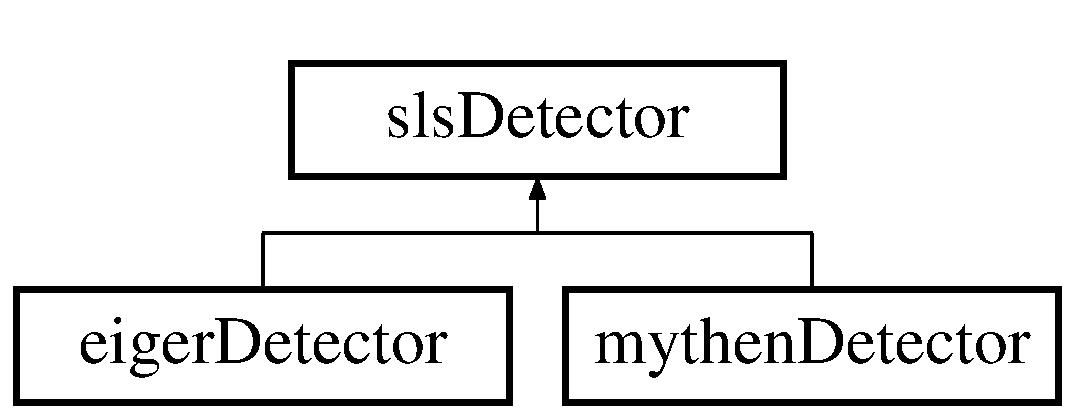
\includegraphics[height=2cm]{classslsDetector}
\end{center}
\end{figure}
\subsection*{Public Types}
\begin{CompactItemize}
\item 
typedef \bf{sls\-Detector::shared\-Sls\-Detector} \bf{shared\-Sls\-Detector}
\begin{CompactList}\small\item\em Structure allocated in shared memory to store detector settings and be accessed in parallel by several applications (take care of possible conflicts!). \item\end{CompactList}\item 
\bf{GET\_\-ONLINE\_\-FLAG}
\item 
\bf{OFFLINE\_\-FLAG}
\item 
\bf{ONLINE\_\-FLAG}
\item 
enum \{ \bf{GET\_\-ONLINE\_\-FLAG}, 
\bf{OFFLINE\_\-FLAG}, 
\bf{ONLINE\_\-FLAG}
 \}
\end{CompactItemize}
\subsection*{Public Member Functions}
\begin{CompactItemize}
\item 
\bf{sls\-Detector} (\bf{detector\-Type} type=GENERIC, int id=0)
\item 
\bf{$\sim$sls\-Detector} ()
\item 
int \bf{set\-Online} (int const online)
\item 
int \bf{exists} ()
\item 
virtual int \bf{read\-Configuration\-File} (string const fname)=0
\item 
virtual int \bf{write\-Configuration\-File} (string const fname)=0
\item 
virtual int \bf{dump\-Detector\-Setup} (string const fname)=0
\item 
virtual int \bf{retrieve\-Detector\-Setup} (string const fname)=0
\item 
int \bf{set\-TCPSocket} (string const name=\char`\"{}\char`\"{}, int const control\_\-port=-1, int const stop\_\-port=-1, int const data\_\-port=-1)
\item 
char $\ast$ \bf{get\-Hostname} ()
\item 
int \bf{get\-Control\-Port} ()
\item 
int \bf{get\-Stop\-Port} ()
\item 
int \bf{get\-Data\-Port} ()
\item 
char $\ast$ \bf{get\-Trim\-Dir} ()
\item 
char $\ast$ \bf{set\-Trim\-Dir} (string s)
\item 
int \bf{get\-Trim\-En} (int $\ast$en=NULL)
\item 
virtual \bf{sls\_\-detector\_\-module} $\ast$ \bf{read\-Trim\-File} (string fname, \bf{sls\_\-detector\_\-module} $\ast$my\-Mod=NULL)=0
\item 
virtual int \bf{write\-Trim\-File} (string fname, \bf{sls\_\-detector\_\-module} mod)=0
\item 
virtual int \bf{write\-Trim\-File} (string fname, int imod)=0
\item 
char $\ast$ \bf{set\-File\-Path} (string s)
\item 
char $\ast$ \bf{set\-File\-Name} (string s)
\item 
int \bf{set\-File\-Index} (int i)
\item 
char $\ast$ \bf{get\-File\-Path} ()
\item 
char $\ast$ \bf{get\-File\-Name} ()
\item 
int \bf{get\-File\-Index} ()
\item 
string \bf{create\-File\-Name} ()
\item 
virtual int \bf{write\-Data\-File} (string fname, float $\ast$data, float $\ast$err=NULL, float $\ast$ang=NULL, char dataformat='f', int nch=-1)=0
\item 
virtual int \bf{write\-Data\-File} (string fname, int $\ast$data)=0
\item 
virtual int \bf{read\-Data\-File} (string fname, float $\ast$data, float $\ast$err=NULL, float $\ast$ang=NULL, char dataformat='f', int nch=0)=0
\item 
virtual int \bf{read\-Data\-File} (string fname, int $\ast$data)=0
\item 
char $\ast$ \bf{get\-Cal\-Dir} ()
\item 
char $\ast$ \bf{set\-Cal\-Dir} (string s)
\item 
virtual int \bf{read\-Calibration\-File} (string fname, float \&gain, float \&offset)=0
\item 
virtual int \bf{write\-Calibration\-File} (string fname, float gain, float offset)=0
\item 
virtual int \bf{read\-Angular\-Conversion} (string fname=\char`\"{}\char`\"{})=0
\item 
virtual int \bf{write\-Angular\-Conversion} (string fname=\char`\"{}\char`\"{})=0
\item 
int \bf{exec\-Command} (string cmd, string answer)
\item 
int \bf{set\-Detector\-Type} (\bf{detector\-Type} type=GET\_\-DETECTOR\_\-TYPE)
\item 
int \bf{set\-Detector\-Type} (string type)
\item 
void \bf{get\-Detector\-Type} (char $\ast$type)
\item 
int \bf{set\-Number\-Of\-Modules} (int n, \bf{dimension} d=X)
\item 
int \bf{get\-Max\-Number\-Of\-Modules} (\bf{dimension} d=X)
\item 
\bf{external\-Signal\-Flag} \bf{set\-External\-Signal\-Flags} (\bf{external\-Signal\-Flag} pol=GET\_\-EXTERNAL\_\-SIGNAL\_\-FLAG, int signalindex=0)
\item 
\bf{external\-Communication\-Mode} \bf{set\-External\-Communication\-Mode} (\bf{external\-Communication\-Mode} pol=GET\_\-EXTERNAL\_\-COMMUNICATION\_\-MODE)
\item 
int64\_\-t \bf{get\-Id} (\bf{id\-Mode} mode, int imod=0)
\item 
int \bf{digital\-Test} (\bf{digital\-Test\-Mode} mode, int imod=0)
\item 
int $\ast$ \bf{analog\-Test} (\bf{analog\-Test\-Mode} mode)
\item 
int \bf{enable\-Analog\-Output} (int ichan)
\item 
int \bf{enable\-Analog\-Output} (int imod, int ichip, int ichan)
\item 
int \bf{give\-Calibration\-Pulse} (float vcal, int npulses)
\item 
int \bf{write\-Register} (int addr, int val)
\item 
int \bf{read\-Register} (int addr)
\item 
float \bf{set\-DAC} (float val, \bf{dac\-Index} index, int imod=-1)
\item 
float \bf{get\-ADC} (\bf{dac\-Index} index, int imod=0)
\item 
int \bf{set\-Channel} (int64\_\-t reg, int ichan=-1, int ichip=-1, int imod=-1)
\item 
int \bf{set\-Channel} (\bf{sls\_\-detector\_\-channel} chan)
\item 
\bf{sls\_\-detector\_\-channel} \bf{get\-Channel} (int ichan, int ichip, int imod)
\item 
int \bf{set\-Chip} (int reg, int ichip=-1, int imod=-1)
\item 
int \bf{set\-Chip} (\bf{sls\_\-detector\_\-chip} chip)
\item 
\bf{sls\_\-detector\_\-chip} \bf{get\-Chip} (int ichip, int imod)
\item 
int \bf{set\-Module} (int reg, int imod=-1)
\item 
int \bf{set\-Module} (\bf{sls\_\-detector\_\-module} module)
\item 
\bf{sls\_\-detector\_\-module} $\ast$ \bf{get\-Module} (int imod)
\item 
int \bf{get\-Threshold\-Energy} (int imod=-1)
\item 
int \bf{set\-Threshold\-Energy} (int e\_\-e\-V, int imod=-1, \bf{detector\-Settings} isettings=GET\_\-SETTINGS)
\item 
\bf{detector\-Settings} \bf{get\-Settings} (int imod=-1)
\item 
\bf{detector\-Settings} \bf{set\-Settings} (\bf{detector\-Settings} isettings, int imod=-1)
\item 
int \bf{start\-Acquisition} ()
\item 
int \bf{stop\-Acquisition} ()
\item 
int \bf{start\-Read\-Out} ()
\item 
int \bf{get\-Run\-Status} ()
\item 
int $\ast$ \bf{start\-And\-Read\-All} ()
\item 
int \bf{start\-And\-Read\-All\-No\-Wait} ()
\item 
int $\ast$ \bf{get\-Data\-From\-Detector\-No\-Wait} ()
\item 
int $\ast$ \bf{read\-Frame} ()
\item 
int $\ast$ \bf{read\-All} ()
\item 
int $\ast$ \bf{pop\-Data\-Queue} ()
\item 
int64\_\-t \bf{set\-Timer} (\bf{timer\-Index} index, int64\_\-t t=-1)
\item 
int64\_\-t \bf{get\-Time\-Left} (\bf{timer\-Index} index)
\item 
int \bf{set\-Speed} (\bf{speed\-Variable} sp, int value=-1)
\item 
int \bf{set\-Dynamic\-Range} (int n=-1)
\item 
int \bf{set\-ROI} (int nroi=-1, int $\ast$xmin=NULL, int $\ast$xmax=NULL, int $\ast$ymin=NULL, int $\ast$ymax=NULL)
\item 
int \bf{set\-Read\-Out\-Flags} (\bf{read\-Out\-Flags} flag)
\item 
int \bf{execute\-Trimming} (\bf{trim\-Mode} mode, int par1, int par2, int imod=-1)
\item 
int \bf{set\-Flat\-Field\-Correction} (string fname=\char`\"{}\char`\"{})
\item 
int \bf{get\-Flat\-Field\-Corrections} (float $\ast$corr=NULL, float $\ast$ecorr=NULL)
\item 
int \bf{set\-Rate\-Correction} (float t=0)
\item 
int \bf{get\-Rate\-Corrections} (float \&t)
\item 
int \bf{get\-Rate\-Corrections} ()
\item 
int \bf{set\-Bad\-Channel\-Correction} (string fname=\char`\"{}\char`\"{})
\item 
int \bf{get\-Bad\-Channel\-Corrections} (int $\ast$bad=NULL)
\item 
char $\ast$ \bf{get\-Bad\-Channel\-Correction\-File} ()
\item 
virtual int \bf{set\-Angular\-Conversion} (string fname=\char`\"{}\char`\"{})=0
\item 
virtual int \bf{get\-Angular\-Conversion} (int \&direction, \bf{angle\-Conversion\-Constant} $\ast$angconv=NULL)=0
\item 
virtual char $\ast$ \bf{get\-Angular\-Conversion} ()=0
\item 
virtual float \bf{set\-Global\-Offset} (float f)=0
\item 
virtual float \bf{set\-Fine\-Offset} (float f)=0
\item 
virtual float \bf{get\-Fine\-Offset} ()=0
\item 
virtual float \bf{get\-Global\-Offset} ()=0
\item 
virtual int \bf{set\-Positions} (int n\-Pos, float $\ast$\bf{pos})=0
\item 
virtual int \bf{get\-Positions} (float $\ast$\bf{pos}=NULL)=0
\item 
virtual float \bf{set\-Bin\-Size} (float bs)=0
\item 
virtual float \bf{get\-Bin\-Size} ()=0
\item 
float $\ast$ \bf{decode\-Data} (int $\ast$datain)
\item 
int \bf{flat\-Field\-Correct} (float datain, float errin, float \&dataout, float \&errout, float ffcoefficient, float fferr)
\item 
int \bf{flat\-Field\-Correct} (float $\ast$datain, float $\ast$errin, float $\ast$dataout, float $\ast$errout)
\item 
int \bf{rate\-Correct} (float datain, float errin, float \&dataout, float \&errout, float tau, float t)
\item 
int \bf{rate\-Correct} (float $\ast$datain, float $\ast$errin, float $\ast$dataout, float $\ast$errout)
\item 
virtual int \bf{reset\-Merging} (float $\ast$mp, float $\ast$mv, float $\ast$me, int $\ast$mm)=0
\item 
virtual int \bf{add\-To\-Merging} (float $\ast$p1, float $\ast$v1, float $\ast$e1, float $\ast$mp, float $\ast$mv, float $\ast$me, int $\ast$mm)=0
\item 
int \bf{finalize\-Merging} (float $\ast$mp, float $\ast$mv, float $\ast$me, int $\ast$mm)
\item 
int \bf{exit\-Server} ()
\item 
virtual void $\ast$ \bf{process\-Data} ()=0
\item 
\bf{sls\_\-detector\_\-module} $\ast$ \bf{create\-Module} ()
\item 
void \bf{delete\-Module} (\bf{sls\_\-detector\_\-module} $\ast$my\-Mod)
\item 
virtual void \bf{acquire} ()=0
\end{CompactItemize}
\subsection*{Protected Member Functions}
\begin{CompactItemize}
\item 
int $\ast$ \bf{get\-Data\-From\-Detector} ()
\item 
int \bf{init\-Shared\-Memory} (\bf{detector\-Type} type=GENERIC, int id=0)
\item 
int \bf{free\-Shared\-Memory} ()
\item 
int \bf{initialize\-Detector\-Size} (\bf{detector\-Type} type)
\item 
int \bf{initialize\-Detector\-Structure} ()
\item 
int \bf{send\-Channel} (\bf{sls\_\-detector\_\-channel} $\ast$)
\item 
int \bf{send\-Chip} (\bf{sls\_\-detector\_\-chip} $\ast$)
\item 
int \bf{send\-Module} (\bf{sls\_\-detector\_\-module} $\ast$)
\item 
int \bf{receive\-Channel} (\bf{sls\_\-detector\_\-channel} $\ast$)
\item 
int \bf{receive\-Chip} (\bf{sls\_\-detector\_\-chip} $\ast$)
\item 
int \bf{receive\-Module} (\bf{sls\_\-detector\_\-module} $\ast$)
\item 
void \bf{start\-Thread} ()
\item 
int \bf{fill\-Bad\-Channel\-Mask} ()
\end{CompactItemize}
\subsection*{Protected Attributes}
\begin{CompactItemize}
\item 
\bf{shared\-Sls\-Detector} $\ast$ \bf{this\-Detector}
\item 
int \bf{online\-Flag}
\item 
int \bf{det\-Id}
\item 
int \bf{shm\-Id}
\item 
\bf{My\-Socket\-TCP} $\ast$ \bf{control\-Socket}
\item 
\bf{My\-Socket\-TCP} $\ast$ \bf{stop\-Socket}
\item 
\bf{My\-Socket\-TCP} $\ast$ \bf{data\-Socket}
\item 
queue$<$ int $\ast$ $>$ \bf{data\-Queue}
\item 
pthread\_\-t \bf{data\-Processing\-Thread}
\item 
float \bf{current\-Position}
\item 
float \bf{current\-Position\-Index}
\item 
float \bf{current\-I0}
\item 
float $\ast$ \bf{merging\-Bins}
\item 
float $\ast$ \bf{merging\-Counts}
\item 
float $\ast$ \bf{merging\-Errors}
\item 
int $\ast$ \bf{merging\-Multiplicity}
\item 
float $\ast$ \bf{ffcoefficients}
\item 
float $\ast$ \bf{fferrors}
\item 
\bf{sls\_\-detector\_\-module} $\ast$ \bf{detector\-Modules}
\item 
float $\ast$ \bf{dacs}
\item 
float $\ast$ \bf{adcs}
\item 
int $\ast$ \bf{chipregs}
\item 
int $\ast$ \bf{chanregs}
\item 
int $\ast$ \bf{bad\-Channel\-Mask}
\end{CompactItemize}
\subsection*{Classes}
\begin{CompactItemize}
\item 
struct \bf{shared\-Sls\-Detector}
\begin{CompactList}\small\item\em Structure allocated in shared memory to store detector settings and be accessed in parallel by several applications (take care of possible conflicts!). \item\end{CompactList}\end{CompactItemize}


\subsection{Detailed Description}
This is the base class for all SLS detector functionalities. 

The \doxyref{sls\-Detector}{p.}{classslsDetector} class is expected to become the interface class for all SLS Detectors acquisition (and analysis) software.

\begin{Desc}
\item[Author:]Anna Bergamaschi \end{Desc}
\begin{Desc}
\item[Version:]0.1alpha \end{Desc}




\subsection{Member Typedef Documentation}
\index{slsDetector@{sls\-Detector}!sharedSlsDetector@{sharedSlsDetector}}
\index{sharedSlsDetector@{sharedSlsDetector}!slsDetector@{sls\-Detector}}
\subsubsection{\setlength{\rightskip}{0pt plus 5cm}typedef struct \bf{sls\-Detector::shared\-Sls\-Detector}  \bf{sls\-Detector::shared\-Sls\-Detector}}\label{classslsDetector_2dd6bff7d94ab8005c2797152b19264e}


Structure allocated in shared memory to store detector settings and be accessed in parallel by several applications (take care of possible conflicts!). 



\subsection{Member Enumeration Documentation}
\subsubsection{\setlength{\rightskip}{0pt plus 5cm}anonymous enum}\label{classslsDetector_ac085f1939dcfed328dc6ff4b11fdb44}


online flags enum\begin{Desc}
\item[See also:]\doxyref{set\-Online}{p.}{classslsDetector_f041f723f702c17de292061d6d609698} \end{Desc}
\begin{Desc}
\item[Enumerator: ]\par
\begin{description}
\index{GET_ONLINE_FLAG@{GET\_\-ONLINE\_\-FLAG}!slsDetector@{slsDetector}}\index{slsDetector@{slsDetector}!GET_ONLINE_FLAG@{GET\_\-ONLINE\_\-FLAG}}\item[{\em 
GET\_\-ONLINE\_\-FLAG\label{classslsDetector_ac085f1939dcfed328dc6ff4b11fdb44617c55ac8cf00235b76c1c1481238abb}
}]returns wether the detector is in online or offline state \index{OFFLINE_FLAG@{OFFLINE\_\-FLAG}!slsDetector@{slsDetector}}\index{slsDetector@{slsDetector}!OFFLINE_FLAG@{OFFLINE\_\-FLAG}}\item[{\em 
OFFLINE\_\-FLAG\label{classslsDetector_ac085f1939dcfed328dc6ff4b11fdb44da0a4f5b33e634292bc99256a9552f2f}
}]detector in offline state (i.e. no communication to the detector - using only local structure - no data acquisition possible!) \index{ONLINE_FLAG@{ONLINE\_\-FLAG}!slsDetector@{slsDetector}}\index{slsDetector@{slsDetector}!ONLINE_FLAG@{ONLINE\_\-FLAG}}\item[{\em 
ONLINE\_\-FLAG\label{classslsDetector_ac085f1939dcfed328dc6ff4b11fdb44d3b612a2eb0d1029bd260b502afcf632}
}]detector in online state (i.e. communication to the detector updating the local structure) \end{description}
\end{Desc}



\subsection{Constructor \& Destructor Documentation}
\index{slsDetector@{sls\-Detector}!slsDetector@{slsDetector}}
\index{slsDetector@{slsDetector}!slsDetector@{sls\-Detector}}
\subsubsection{\setlength{\rightskip}{0pt plus 5cm}sls\-Detector::sls\-Detector (\bf{detector\-Type} {\em type} = {\tt GENERIC}, int {\em id} = {\tt 0})}\label{classslsDetector_eea9fc044ff9d496e4338efaaf176498}


(default) constructor \begin{Desc}
\item[Parameters:]
\begin{description}
\item[{\em type}]is needed to define the size of the detector shared memory 9defaults to GENERIC i.e. the largest shared memory needed by any \doxyref{sls\-Detector}{p.}{classslsDetector} is allocated \item[{\em id}]is the detector index which is needed to define the shared memory id. Different physical detectors should have different IDs in order to work independently \end{description}
\end{Desc}


sets online\-Flag to OFFLINE\_\-FLAG

Initlializes shared memory \begin{Desc}
\item[See also:]\doxyref{init\-Shared\-Memory}{p.}{classslsDetector_cb94b9bfa7bbea2d9e1b0289a272bca8}\end{Desc}
if it fails the detector id is incremented until it succeeds

Initializes the detector stucture \begin{Desc}
\item[See also:]\doxyref{initialize\-Detector\-Size}{p.}{classslsDetector_19f1c6d120293c98a0d2dc992e5616f8} \end{Desc}
\index{slsDetector@{sls\-Detector}!~slsDetector@{$\sim$slsDetector}}
\index{~slsDetector@{$\sim$slsDetector}!slsDetector@{sls\-Detector}}
\subsubsection{\setlength{\rightskip}{0pt plus 5cm}sls\-Detector::$\sim$sls\-Detector ()\hspace{0.3cm}{\tt  [inline]}}\label{classslsDetector_7653e532ff88dbf403e270769bccc509}


destructor 

\subsection{Member Function Documentation}
\index{slsDetector@{sls\-Detector}!acquire@{acquire}}
\index{acquire@{acquire}!slsDetector@{sls\-Detector}}
\subsubsection{\setlength{\rightskip}{0pt plus 5cm}virtual void sls\-Detector::acquire ()\hspace{0.3cm}{\tt  [pure virtual]}}\label{classslsDetector_d2ee30dfd50f06431dca4e4b9619f301}


pure virtual function performs the complete acquisition and data processing moves the detector to next position \par
 starts and reads the detector \par
 reads the IC (if required) \par
 reads the encoder (iof required for angualr conversion) \par
 processes the data (flat field, rate, angular conversion and merging process\-Data()) \begin{Desc}
\item[See also:]\doxyref{mythen\-Detector::acquire()}{p.}{classmythenDetector_bb3d2f51a414cf9dace29a4b5676828f} \end{Desc}


Implemented in \bf{mythen\-Detector} \doxyref{p.}{classmythenDetector_bb3d2f51a414cf9dace29a4b5676828f}.\index{slsDetector@{sls\-Detector}!addToMerging@{addToMerging}}
\index{addToMerging@{addToMerging}!slsDetector@{sls\-Detector}}
\subsubsection{\setlength{\rightskip}{0pt plus 5cm}virtual int sls\-Detector::add\-To\-Merging (float $\ast$ {\em p1}, float $\ast$ {\em v1}, float $\ast$ {\em e1}, float $\ast$ {\em mp}, float $\ast$ {\em mv}, float $\ast$ {\em me}, int $\ast$ {\em mm})\hspace{0.3cm}{\tt  [pure virtual]}}\label{classslsDetector_feb8730f24292620e5d451cd2d4bb9cd}


pure virtual function merge dataset \begin{Desc}
\item[Parameters:]
\begin{description}
\item[{\em p1}]angular positions of dataset \item[{\em v1}]data \item[{\em e1}]errors \item[{\em mp}]already merged postions \item[{\em mv}]already merged data \item[{\em me}]already merged errors (squared sum) \item[{\em mm}]multiplicity of merged arrays \end{description}
\end{Desc}
\begin{Desc}
\item[See also:]\doxyref{mythen\-Detector::add\-To\-Merging}{p.}{classmythenDetector_eaaf7d7e3150f473e3bbcf59d91692c2} \end{Desc}


Implemented in \bf{mythen\-Detector} \doxyref{p.}{classmythenDetector_eaaf7d7e3150f473e3bbcf59d91692c2}.\index{slsDetector@{sls\-Detector}!analogTest@{analogTest}}
\index{analogTest@{analogTest}!slsDetector@{sls\-Detector}}
\subsubsection{\setlength{\rightskip}{0pt plus 5cm}int$\ast$ sls\-Detector::analog\-Test (\bf{analog\-Test\-Mode} {\em mode})}\label{classslsDetector_18f91f8cf70d2d4eef9b3488b90bac51}


analog test \begin{Desc}
\item[Parameters:]
\begin{description}
\item[{\em modte}]test mode \end{description}
\end{Desc}
\begin{Desc}
\item[Returns:]pointer to acquired data\end{Desc}
not yet implemented \index{slsDetector@{sls\-Detector}!createFileName@{createFileName}}
\index{createFileName@{createFileName}!slsDetector@{sls\-Detector}}
\subsubsection{\setlength{\rightskip}{0pt plus 5cm}string sls\-Detector::create\-File\-Name ()}\label{classslsDetector_d055c470ae6faa973980f4dbf021132d}


generates file name without extension

always appends to file path and file name the run index.

in case also appends the position index

Filenames will be of the form: filepath/filename(\_\-px)\_\-i where x is the position index and i is the run index \index{slsDetector@{sls\-Detector}!createModule@{createModule}}
\index{createModule@{createModule}!slsDetector@{sls\-Detector}}
\subsubsection{\setlength{\rightskip}{0pt plus 5cm}\bf{sls\_\-detector\_\-module} $\ast$ sls\-Detector::create\-Module ()}\label{classslsDetector_b1d4c6c01d1e10fe06bc83329410d4f4}


Allocates the memory for a \doxyref{sls\_\-detector\_\-module}{p.}{structsls__detector__module} structure and initializes it \begin{Desc}
\item[Returns:]my\-Mod the pointer to the allocate dmemory location \end{Desc}
\index{slsDetector@{sls\-Detector}!decodeData@{decodeData}}
\index{decodeData@{decodeData}!slsDetector@{sls\-Detector}}
\subsubsection{\setlength{\rightskip}{0pt plus 5cm}float $\ast$ sls\-Detector::decode\-Data (int $\ast$ {\em datain})}\label{classslsDetector_937d257464bade6dc6d3ab42c86843ba}


decode data from the detector converting them to an array of floats, one for each channle \begin{Desc}
\item[Parameters:]
\begin{description}
\item[{\em datain}]data from the detector \end{description}
\end{Desc}
\begin{Desc}
\item[Returns:]pointer to a float array with a data per channel \end{Desc}


Reimplemented in \bf{eiger\-Detector} \doxyref{p.}{classeigerDetector_3e0573baf38c37818c7769fb351010b3}.\index{slsDetector@{sls\-Detector}!deleteModule@{deleteModule}}
\index{deleteModule@{deleteModule}!slsDetector@{sls\-Detector}}
\subsubsection{\setlength{\rightskip}{0pt plus 5cm}void sls\-Detector::delete\-Module (\bf{sls\_\-detector\_\-module} $\ast$ {\em my\-Mod})}\label{classslsDetector_48984c8d058355c5249233165bf0c410}


frees the memory for a \doxyref{sls\_\-detector\_\-module}{p.}{structsls__detector__module} structure \begin{Desc}
\item[Parameters:]
\begin{description}
\item[{\em my\-Mod}]the pointer to the memory to be freed \end{description}
\end{Desc}
\index{slsDetector@{sls\-Detector}!digitalTest@{digitalTest}}
\index{digitalTest@{digitalTest}!slsDetector@{sls\-Detector}}
\subsubsection{\setlength{\rightskip}{0pt plus 5cm}int sls\-Detector::digital\-Test (\bf{digital\-Test\-Mode} {\em mode}, int {\em imod} = {\tt 0})}\label{classslsDetector_40906e79010db5b8082d4855a3824aa7}


Digital test of the modules \begin{Desc}
\item[Parameters:]
\begin{description}
\item[{\em mode}]test mode \item[{\em imod}]module number for chip test or module firmware test \end{description}
\end{Desc}
\begin{Desc}
\item[Returns:]OK or error mask \end{Desc}
\index{slsDetector@{sls\-Detector}!dumpDetectorSetup@{dumpDetectorSetup}}
\index{dumpDetectorSetup@{dumpDetectorSetup}!slsDetector@{sls\-Detector}}
\subsubsection{\setlength{\rightskip}{0pt plus 5cm}virtual int sls\-Detector::dump\-Detector\-Setup (string const  {\em fname})\hspace{0.3cm}{\tt  [pure virtual]}}\label{classslsDetector_96428855d6e286408a52e675e045cf45}


Purely virtual function Should be implemented in the specific detector class /sa \doxyref{mythen\-Detector::dump\-Detector\-Setup}{p.}{classmythenDetector_a0fe9987e8fa240a312ad353ae539188} 

Implemented in \bf{mythen\-Detector} \doxyref{p.}{classmythenDetector_a0fe9987e8fa240a312ad353ae539188}.\index{slsDetector@{sls\-Detector}!enableAnalogOutput@{enableAnalogOutput}}
\index{enableAnalogOutput@{enableAnalogOutput}!slsDetector@{sls\-Detector}}
\subsubsection{\setlength{\rightskip}{0pt plus 5cm}int sls\-Detector::enable\-Analog\-Output (int {\em imod}, int {\em ichip}, int {\em ichan})}\label{classslsDetector_b20fef344ee47114fccb4d1bc8c6e5bd}


enable analog output of channel ichan, chip ichip, module imod

not yet implemented \index{slsDetector@{sls\-Detector}!enableAnalogOutput@{enableAnalogOutput}}
\index{enableAnalogOutput@{enableAnalogOutput}!slsDetector@{sls\-Detector}}
\subsubsection{\setlength{\rightskip}{0pt plus 5cm}int sls\-Detector::enable\-Analog\-Output (int {\em ichan})}\label{classslsDetector_a83074759c48f194af2e45d1281cc818}


enable analog output of channel ichan

not yet implemented \index{slsDetector@{sls\-Detector}!execCommand@{execCommand}}
\index{execCommand@{execCommand}!slsDetector@{sls\-Detector}}
\subsubsection{\setlength{\rightskip}{0pt plus 5cm}int sls\-Detector::exec\-Command (string {\em cmd}, string {\em answer})}\label{classslsDetector_9fc0c9161e967094a535cc40bc33cc6b}


executes a system command on the server e.g. mount an nfs disk, reboot and returns answer etc. \begin{Desc}
\item[Parameters:]
\begin{description}
\item[{\em cmd}]is the command to be executed \item[{\em answer}]is the answer from the detector \end{description}
\end{Desc}
\begin{Desc}
\item[Returns:]OK or FAIL depending on the command outcome \end{Desc}
\index{slsDetector@{sls\-Detector}!executeTrimming@{executeTrimming}}
\index{executeTrimming@{executeTrimming}!slsDetector@{sls\-Detector}}
\subsubsection{\setlength{\rightskip}{0pt plus 5cm}int sls\-Detector::execute\-Trimming (\bf{trim\-Mode} {\em mode}, int {\em par1}, int {\em par2}, int {\em imod} = {\tt -1})}\label{classslsDetector_a257317d18965a353679c66b15b0987d}


execute trimming \begin{Desc}
\item[Parameters:]
\begin{description}
\item[{\em mode}]trim mode \item[{\em par1}]if noise, beam or fixed setting trimming it is count limit, if improve maximum number of iterations \item[{\em par2}]if noise or beam nsigma, if improve par2!=means vthreshold will be optimized, if fixed settings par2$<$0 trimwith median, par2$>$=0 trim with level \item[{\em imod}]module number (-1 all) \end{description}
\end{Desc}
\begin{Desc}
\item[Returns:]OK or FAIl (FAIL also if some channel are 0 or 63 \end{Desc}
\index{slsDetector@{sls\-Detector}!exists@{exists}}
\index{exists@{exists}!slsDetector@{sls\-Detector}}
\subsubsection{\setlength{\rightskip}{0pt plus 5cm}int sls\-Detector::exists ()\hspace{0.3cm}{\tt  [inline]}}\label{classslsDetector_bf592960cebe5b3f1e2fdc77f770f17a}


sets the online\-Flag \begin{Desc}
\item[Returns:]1 if the detector structure has already be initlialized, 0 otherwise \end{Desc}
\index{slsDetector@{sls\-Detector}!exitServer@{exitServer}}
\index{exitServer@{exitServer}!slsDetector@{sls\-Detector}}
\subsubsection{\setlength{\rightskip}{0pt plus 5cm}int sls\-Detector::exit\-Server ()}\label{classslsDetector_466e9a65aa0b404c771d70c9f01af8b9}


turns off server \index{slsDetector@{sls\-Detector}!fillBadChannelMask@{fillBadChannelMask}}
\index{fillBadChannelMask@{fillBadChannelMask}!slsDetector@{sls\-Detector}}
\subsubsection{\setlength{\rightskip}{0pt plus 5cm}int sls\-Detector::fill\-Bad\-Channel\-Mask ()\hspace{0.3cm}{\tt  [protected]}}\label{classslsDetector_6a0ebe013e27c065b2f67158a27f64ac}


fill bad channel mask (0 if channel is good, 1 if bad) \index{slsDetector@{sls\-Detector}!finalizeMerging@{finalizeMerging}}
\index{finalizeMerging@{finalizeMerging}!slsDetector@{sls\-Detector}}
\subsubsection{\setlength{\rightskip}{0pt plus 5cm}int sls\-Detector::finalize\-Merging (float $\ast$ {\em mp}, float $\ast$ {\em mv}, float $\ast$ {\em me}, int $\ast$ {\em mm})}\label{classslsDetector_8f73479f68ca2171fd2108c2f157299e}


pure virtual function calculates the \char`\"{}final\char`\"{} positions, data value and errors for the emrged data \begin{Desc}
\item[Parameters:]
\begin{description}
\item[{\em mp}]already merged postions \item[{\em mv}]already merged data \item[{\em me}]already merged errors (squared sum) \item[{\em mm}]multiplicity of merged arrays \end{description}
\end{Desc}
\begin{Desc}
\item[Returns:]FAIL or the number of non empty bins (i.e. points belonging to the pattern) \end{Desc}
\begin{Desc}
\item[See also:]\doxyref{mythen\-Detector::finalize\-Merging}{p.}{classmythenDetector_a919a42bd89fe21c4086bae5f1fb2f32} \end{Desc}


Reimplemented in \bf{mythen\-Detector} \doxyref{p.}{classmythenDetector_a919a42bd89fe21c4086bae5f1fb2f32}.\index{slsDetector@{sls\-Detector}!flatFieldCorrect@{flatFieldCorrect}}
\index{flatFieldCorrect@{flatFieldCorrect}!slsDetector@{sls\-Detector}}
\subsubsection{\setlength{\rightskip}{0pt plus 5cm}int sls\-Detector::flat\-Field\-Correct (float $\ast$ {\em datain}, float $\ast$ {\em errin}, float $\ast$ {\em dataout}, float $\ast$ {\em errout})}\label{classslsDetector_1e6633db752222079b39a187e4d0e658}


flat field correct data \begin{Desc}
\item[Parameters:]
\begin{description}
\item[{\em datain}]data array \item[{\em errin}]error array on data (if NULL will default to sqrt(datain) \item[{\em dataout}]array of corrected data \item[{\em errout}]error on corrected data (if not NULL) \end{description}
\end{Desc}
\begin{Desc}
\item[Returns:]0 \end{Desc}
\index{slsDetector@{sls\-Detector}!flatFieldCorrect@{flatFieldCorrect}}
\index{flatFieldCorrect@{flatFieldCorrect}!slsDetector@{sls\-Detector}}
\subsubsection{\setlength{\rightskip}{0pt plus 5cm}int sls\-Detector::flat\-Field\-Correct (float {\em datain}, float {\em errin}, float \& {\em dataout}, float \& {\em errout}, float {\em ffcoefficient}, float {\em fferr})}\label{classslsDetector_24c7dd58e00df0bf62221b7572430740}


flat field correct data \begin{Desc}
\item[Parameters:]
\begin{description}
\item[{\em datain}]data \item[{\em errin}]error on data (if$<$=0 will default to sqrt(datain) \item[{\em dataout}]corrected data \item[{\em errout}]error on corrected data \item[{\em ffcoefficient}]flat field correction coefficient \item[{\em fferr}]erro on ffcoefficient \end{description}
\end{Desc}
\begin{Desc}
\item[Returns:]0 \end{Desc}
\index{slsDetector@{sls\-Detector}!freeSharedMemory@{freeSharedMemory}}
\index{freeSharedMemory@{freeSharedMemory}!slsDetector@{sls\-Detector}}
\subsubsection{\setlength{\rightskip}{0pt plus 5cm}int sls\-Detector::free\-Shared\-Memory ()\hspace{0.3cm}{\tt  [protected]}}\label{classslsDetector_5de7fb0d82ae2bcc406385373e665c6f}


Frees the shared memory - should not be used \index{slsDetector@{sls\-Detector}!getADC@{getADC}}
\index{getADC@{getADC}!slsDetector@{sls\-Detector}}
\subsubsection{\setlength{\rightskip}{0pt plus 5cm}float sls\-Detector::get\-ADC (\bf{dac\-Index} {\em index}, int {\em imod} = {\tt 0})}\label{classslsDetector_fa99bd04043c23b7ab583159dabebf93}


set dacs value \begin{Desc}
\item[Parameters:]
\begin{description}
\item[{\em index}]ADC index \item[{\em imod}]module number \end{description}
\end{Desc}
\begin{Desc}
\item[Returns:]current ADC value \end{Desc}
\index{slsDetector@{sls\-Detector}!getAngularConversion@{getAngularConversion}}
\index{getAngularConversion@{getAngularConversion}!slsDetector@{sls\-Detector}}
\subsubsection{\setlength{\rightskip}{0pt plus 5cm}virtual char$\ast$ sls\-Detector::get\-Angular\-Conversion ()\hspace{0.3cm}{\tt  [pure virtual]}}\label{classslsDetector_0c2e502441fd74ec7fc20604c5c08c27}


pure virtual function returns the angular conversion file \begin{Desc}
\item[See also:]\doxyref{mythen\-Detector::get\-Angular\-Conversion}{p.}{classmythenDetector_b2b2f17c36883323ad0abf762c63494f} \end{Desc}


Implemented in \bf{mythen\-Detector} \doxyref{p.}{classmythenDetector_fab45faa264e44178fc52300eaf92cad}.\index{slsDetector@{sls\-Detector}!getAngularConversion@{getAngularConversion}}
\index{getAngularConversion@{getAngularConversion}!slsDetector@{sls\-Detector}}
\subsubsection{\setlength{\rightskip}{0pt plus 5cm}virtual int sls\-Detector::get\-Angular\-Conversion (int \& {\em direction}, \bf{angle\-Conversion\-Constant} $\ast$ {\em angconv} = {\tt NULL})\hspace{0.3cm}{\tt  [pure virtual]}}\label{classslsDetector_a110e9eb82123756cf89fda0a4cb464d}


pure virtual function get angular conversion \begin{Desc}
\item[Parameters:]
\begin{description}
\item[{\em reference}]to diffractometer direction \item[{\em angconv}]array that will be filled with the angular conversion constants \end{description}
\end{Desc}
\begin{Desc}
\item[Returns:]0 if angular conversion disabled, $>$0 otherwise \end{Desc}
\begin{Desc}
\item[See also:]\doxyref{mythen\-Detector::get\-Angular\-Conversion}{p.}{classmythenDetector_b2b2f17c36883323ad0abf762c63494f} \end{Desc}


Implemented in \bf{mythen\-Detector} \doxyref{p.}{classmythenDetector_b2b2f17c36883323ad0abf762c63494f}.\index{slsDetector@{sls\-Detector}!getBadChannelCorrectionFile@{getBadChannelCorrectionFile}}
\index{getBadChannelCorrectionFile@{getBadChannelCorrectionFile}!slsDetector@{sls\-Detector}}
\subsubsection{\setlength{\rightskip}{0pt plus 5cm}char$\ast$ sls\-Detector::get\-Bad\-Channel\-Correction\-File ()\hspace{0.3cm}{\tt  [inline]}}\label{classslsDetector_0b562f90b64c80e3eb64e9e2153bb234}


returns the bad channel list file \index{slsDetector@{sls\-Detector}!getBadChannelCorrections@{getBadChannelCorrections}}
\index{getBadChannelCorrections@{getBadChannelCorrections}!slsDetector@{sls\-Detector}}
\subsubsection{\setlength{\rightskip}{0pt plus 5cm}int sls\-Detector::get\-Bad\-Channel\-Corrections (int $\ast$ {\em bad} = {\tt NULL})}\label{classslsDetector_f80db913b55026bb69d35585b08729cc}


get bad channels correction \begin{Desc}
\item[Parameters:]
\begin{description}
\item[{\em bad}]pointer to array that if bad!=NULL will be filled with the bad channel list \end{description}
\end{Desc}
\begin{Desc}
\item[Returns:]0 if bad channel disabled or no bad channels, $>$0 otherwise \end{Desc}
\index{slsDetector@{sls\-Detector}!getBinSize@{getBinSize}}
\index{getBinSize@{getBinSize}!slsDetector@{sls\-Detector}}
\subsubsection{\setlength{\rightskip}{0pt plus 5cm}virtual float sls\-Detector::get\-Bin\-Size ()\hspace{0.3cm}{\tt  [pure virtual]}}\label{classslsDetector_7d83754e3f41042caa9297da9a33b714}


pure virtual function return detector bin size used for merging (approx angular resolution) \begin{Desc}
\item[See also:]\doxyref{mythen\-Detector::get\-Bin\-Size}{p.}{classmythenDetector_9fd4e479d7eb3f9c53d5d56a43bbccaf} \end{Desc}


Implemented in \bf{mythen\-Detector} \doxyref{p.}{classmythenDetector_9fd4e479d7eb3f9c53d5d56a43bbccaf}.\index{slsDetector@{sls\-Detector}!getCalDir@{getCalDir}}
\index{getCalDir@{getCalDir}!slsDetector@{sls\-Detector}}
\subsubsection{\setlength{\rightskip}{0pt plus 5cm}char$\ast$ sls\-Detector::get\-Cal\-Dir ()\hspace{0.3cm}{\tt  [inline]}}\label{classslsDetector_102679594e60ed261daff24b4aeac21a}


returns the location of the calibration files \begin{Desc}
\item[See also:]\doxyref{shared\-Sls\-Detector}{p.}{structslsDetector_1_1sharedSlsDetector} \end{Desc}
\index{slsDetector@{sls\-Detector}!getChannel@{getChannel}}
\index{getChannel@{getChannel}!slsDetector@{sls\-Detector}}
\subsubsection{\setlength{\rightskip}{0pt plus 5cm}\bf{sls\_\-detector\_\-channel} sls\-Detector::get\-Channel (int {\em ichan}, int {\em ichip}, int {\em imod})}\label{classslsDetector_05f1a170b7416db77bf7cff762e9b58a}


get channel \begin{Desc}
\item[Parameters:]
\begin{description}
\item[{\em ichan}]channel number \item[{\em ichip}]chip number \item[{\em imod}]module number \end{description}
\end{Desc}
\begin{Desc}
\item[Returns:]current channel structure for channel \end{Desc}
\index{slsDetector@{sls\-Detector}!getChip@{getChip}}
\index{getChip@{getChip}!slsDetector@{sls\-Detector}}
\subsubsection{\setlength{\rightskip}{0pt plus 5cm}\bf{sls\_\-detector\_\-chip} sls\-Detector::get\-Chip (int {\em ichip}, int {\em imod})}\label{classslsDetector_2eb7f887a72cc80d6b00cadd4731e672}


get chip \begin{Desc}
\item[Parameters:]
\begin{description}
\item[{\em ichip}]chip number \item[{\em imod}]module number \end{description}
\end{Desc}
\begin{Desc}
\item[Returns:]current chip structure for channel\end{Desc}
\begin{Desc}
\item[\bf{Bug}]probably does not return corretly! \end{Desc}
\index{slsDetector@{sls\-Detector}!getControlPort@{getControlPort}}
\index{getControlPort@{getControlPort}!slsDetector@{sls\-Detector}}
\subsubsection{\setlength{\rightskip}{0pt plus 5cm}int sls\-Detector::get\-Control\-Port ()\hspace{0.3cm}{\tt  [inline]}}\label{classslsDetector_40ffd69f1c40b26575954e826cdf606a}


returns the detector control port\begin{Desc}
\item[See also:]\doxyref{shared\-Sls\-Detector}{p.}{structslsDetector_1_1sharedSlsDetector} \end{Desc}
\index{slsDetector@{sls\-Detector}!getDataFromDetector@{getDataFromDetector}}
\index{getDataFromDetector@{getDataFromDetector}!slsDetector@{sls\-Detector}}
\subsubsection{\setlength{\rightskip}{0pt plus 5cm}int $\ast$ sls\-Detector::get\-Data\-From\-Detector ()\hspace{0.3cm}{\tt  [protected]}}\label{classslsDetector_b1982e89f8e8de63c807a707ccba594c}


Receives a data frame from the detector socket \begin{Desc}
\item[Returns:]pointer to the data (or NULL if failed) \end{Desc}
\index{slsDetector@{sls\-Detector}!getDataFromDetectorNoWait@{getDataFromDetectorNoWait}}
\index{getDataFromDetectorNoWait@{getDataFromDetectorNoWait}!slsDetector@{sls\-Detector}}
\subsubsection{\setlength{\rightskip}{0pt plus 5cm}int $\ast$ sls\-Detector::get\-Data\-From\-Detector\-No\-Wait ()}\label{classslsDetector_5b678231f1a0fafc518a95b6e58f00a8}


receives a data frame from the detector socket \begin{Desc}
\item[Returns:]pointer to the data or NULL. If NULL disconnects the socket \end{Desc}
\begin{Desc}
\item[See also:]\doxyref{get\-Data\-From\-Detector}{p.}{classslsDetector_b1982e89f8e8de63c807a707ccba594c} \end{Desc}
\index{slsDetector@{sls\-Detector}!getDataPort@{getDataPort}}
\index{getDataPort@{getDataPort}!slsDetector@{sls\-Detector}}
\subsubsection{\setlength{\rightskip}{0pt plus 5cm}int sls\-Detector::get\-Data\-Port ()\hspace{0.3cm}{\tt  [inline]}}\label{classslsDetector_35043766eecb3d760fd95d891bed8b16}


returns the detector data port\begin{Desc}
\item[See also:]\doxyref{shared\-Sls\-Detector}{p.}{structslsDetector_1_1sharedSlsDetector} \end{Desc}
\index{slsDetector@{sls\-Detector}!getDetectorType@{getDetectorType}}
\index{getDetectorType@{getDetectorType}!slsDetector@{sls\-Detector}}
\subsubsection{\setlength{\rightskip}{0pt plus 5cm}void sls\-Detector::get\-Detector\-Type (char $\ast$ {\em type})}\label{classslsDetector_d63d6420e411ff4b962930d9c4fd615d}


gets detector type normally the detector knows what type of detector it is \begin{Desc}
\item[Parameters:]
\begin{description}
\item[{\em type}]is the string where the detector type will be written (\char`\"{}Mythen\char`\"{}, \char`\"{}Pilatus\char`\"{}, \char`\"{}XFS\char`\"{}, \char`\"{}Gotthard\char`\"{}, Agipd\char`\"{}) \end{description}
\end{Desc}
\index{slsDetector@{sls\-Detector}!getFileIndex@{getFileIndex}}
\index{getFileIndex@{getFileIndex}!slsDetector@{sls\-Detector}}
\subsubsection{\setlength{\rightskip}{0pt plus 5cm}int sls\-Detector::get\-File\-Index ()\hspace{0.3cm}{\tt  [inline]}}\label{classslsDetector_68b41fa20ddd8c6c67ac00dfea3c9796}


returns the default output file index \begin{Desc}
\item[See also:]\doxyref{shared\-Sls\-Detector}{p.}{structslsDetector_1_1sharedSlsDetector} \end{Desc}
\index{slsDetector@{sls\-Detector}!getFileName@{getFileName}}
\index{getFileName@{getFileName}!slsDetector@{sls\-Detector}}
\subsubsection{\setlength{\rightskip}{0pt plus 5cm}char$\ast$ sls\-Detector::get\-File\-Name ()\hspace{0.3cm}{\tt  [inline]}}\label{classslsDetector_717a3c59681f81ceaf5245a073eeacdb}


returns the default output files root name \begin{Desc}
\item[See also:]\doxyref{shared\-Sls\-Detector}{p.}{structslsDetector_1_1sharedSlsDetector} \end{Desc}
\index{slsDetector@{sls\-Detector}!getFilePath@{getFilePath}}
\index{getFilePath@{getFilePath}!slsDetector@{sls\-Detector}}
\subsubsection{\setlength{\rightskip}{0pt plus 5cm}char$\ast$ sls\-Detector::get\-File\-Path ()\hspace{0.3cm}{\tt  [inline]}}\label{classslsDetector_b4158bdacd10fccedeab9eacbd1f4304}


returns the default output files path \begin{Desc}
\item[See also:]\doxyref{shared\-Sls\-Detector}{p.}{structslsDetector_1_1sharedSlsDetector} \end{Desc}
\index{slsDetector@{sls\-Detector}!getFineOffset@{getFineOffset}}
\index{getFineOffset@{getFineOffset}!slsDetector@{sls\-Detector}}
\subsubsection{\setlength{\rightskip}{0pt plus 5cm}virtual float sls\-Detector::get\-Fine\-Offset ()\hspace{0.3cm}{\tt  [pure virtual]}}\label{classslsDetector_8e39680a1a096ca13ed672504b5b08e6}


pure virtual function get detector fine offset \begin{Desc}
\item[See also:]\doxyref{mythen\-Detector::get\-Fine\-Offset}{p.}{classmythenDetector_00720f1445f3f301fa3316828d978de6} \end{Desc}


Implemented in \bf{mythen\-Detector} \doxyref{p.}{classmythenDetector_00720f1445f3f301fa3316828d978de6}.\index{slsDetector@{sls\-Detector}!getFlatFieldCorrections@{getFlatFieldCorrections}}
\index{getFlatFieldCorrections@{getFlatFieldCorrections}!slsDetector@{sls\-Detector}}
\subsubsection{\setlength{\rightskip}{0pt plus 5cm}int sls\-Detector::get\-Flat\-Field\-Corrections (float $\ast$ {\em corr} = {\tt NULL}, float $\ast$ {\em ecorr} = {\tt NULL})}\label{classslsDetector_af22c79193907e364c6db97f5e55b9fd}


get flat field corrections \begin{Desc}
\item[Parameters:]
\begin{description}
\item[{\em corr}]if !=NULL will be filled with the correction coefficients \item[{\em ecorr}]if !=NULL will be filled with the correction coefficients errors \end{description}
\end{Desc}
\begin{Desc}
\item[Returns:]0 if ff correction disabled, $>$0 otherwise \end{Desc}
\index{slsDetector@{sls\-Detector}!getGlobalOffset@{getGlobalOffset}}
\index{getGlobalOffset@{getGlobalOffset}!slsDetector@{sls\-Detector}}
\subsubsection{\setlength{\rightskip}{0pt plus 5cm}virtual float sls\-Detector::get\-Global\-Offset ()\hspace{0.3cm}{\tt  [pure virtual]}}\label{classslsDetector_8964e3efa73f29b04bd9479578bd1c59}


pure virtual function get detector global offset \begin{Desc}
\item[See also:]\doxyref{mythen\-Detector::get\-Global\-Offset}{p.}{classmythenDetector_b2086f336d7198381453556b520dd556} \end{Desc}


Implemented in \bf{mythen\-Detector} \doxyref{p.}{classmythenDetector_b2086f336d7198381453556b520dd556}.\index{slsDetector@{sls\-Detector}!getHostname@{getHostname}}
\index{getHostname@{getHostname}!slsDetector@{sls\-Detector}}
\subsubsection{\setlength{\rightskip}{0pt plus 5cm}char$\ast$ sls\-Detector::get\-Hostname ()\hspace{0.3cm}{\tt  [inline]}}\label{classslsDetector_fad06908ad59bfd8a8577899d6aa1843}


returns the detector hostname\begin{Desc}
\item[See also:]\doxyref{shared\-Sls\-Detector}{p.}{structslsDetector_1_1sharedSlsDetector} \end{Desc}
\index{slsDetector@{sls\-Detector}!getId@{getId}}
\index{getId@{getId}!slsDetector@{sls\-Detector}}
\subsubsection{\setlength{\rightskip}{0pt plus 5cm}int64\_\-t sls\-Detector::get\-Id (\bf{id\-Mode} {\em mode}, int {\em imod} = {\tt 0})}\label{classslsDetector_92f9261c62652e3643eebfdfa9942099}


get detector ids/versions for module \begin{Desc}
\item[Parameters:]
\begin{description}
\item[{\em mode}]which id/version has to be read \item[{\em imod}]module number for module serial number \end{description}
\end{Desc}
\begin{Desc}
\item[Returns:]id \end{Desc}
\index{slsDetector@{sls\-Detector}!getMaxNumberOfModules@{getMaxNumberOfModules}}
\index{getMaxNumberOfModules@{getMaxNumberOfModules}!slsDetector@{sls\-Detector}}
\subsubsection{\setlength{\rightskip}{0pt plus 5cm}int sls\-Detector::get\-Max\-Number\-Of\-Modules (\bf{dimension} {\em d} = {\tt X})}\label{classslsDetector_d608a77a1c64989ad82175991be0a9b5}


get the maximum size of the detector \begin{Desc}
\item[Parameters:]
\begin{description}
\item[{\em d}]dimension \end{description}
\end{Desc}
\begin{Desc}
\item[Returns:]maximum number of modules that can be installed in direction d \end{Desc}
\index{slsDetector@{sls\-Detector}!getModule@{getModule}}
\index{getModule@{getModule}!slsDetector@{sls\-Detector}}
\subsubsection{\setlength{\rightskip}{0pt plus 5cm}\bf{sls\_\-detector\_\-module} $\ast$ sls\-Detector::get\-Module (int {\em imod})}\label{classslsDetector_32557eee02e541840246b4b4a3e76c83}


get module \begin{Desc}
\item[Parameters:]
\begin{description}
\item[{\em imod}]module number \end{description}
\end{Desc}
\begin{Desc}
\item[Returns:]pointer to module structure (which has bee created and must then be deleted) \end{Desc}
\index{slsDetector@{sls\-Detector}!getPositions@{getPositions}}
\index{getPositions@{getPositions}!slsDetector@{sls\-Detector}}
\subsubsection{\setlength{\rightskip}{0pt plus 5cm}virtual int sls\-Detector::get\-Positions (float $\ast$ {\em pos} = {\tt NULL})\hspace{0.3cm}{\tt  [pure virtual]}}\label{classslsDetector_248794801b9794d20e7d58bceab564ab}


pure virtual function get positions for the acquisition \begin{Desc}
\item[Parameters:]
\begin{description}
\item[{\em pos}]array which will contain the encoder positions \end{description}
\end{Desc}
\begin{Desc}
\item[Returns:]number of positions \end{Desc}
\begin{Desc}
\item[See also:]\doxyref{mythen\-Detector::get\-Positions}{p.}{classmythenDetector_0d306720dced0d3576474978b06b4be4} \end{Desc}


Implemented in \bf{mythen\-Detector} \doxyref{p.}{classmythenDetector_0d306720dced0d3576474978b06b4be4}.\index{slsDetector@{sls\-Detector}!getRateCorrections@{getRateCorrections}}
\index{getRateCorrections@{getRateCorrections}!slsDetector@{sls\-Detector}}
\subsubsection{\setlength{\rightskip}{0pt plus 5cm}int sls\-Detector::get\-Rate\-Corrections ()}\label{classslsDetector_7606366a3cbe280c90dc659036814697}


get rate correction \begin{Desc}
\item[Returns:]0 if rate correction disabled, $>$0 otherwise \end{Desc}
\index{slsDetector@{sls\-Detector}!getRateCorrections@{getRateCorrections}}
\index{getRateCorrections@{getRateCorrections}!slsDetector@{sls\-Detector}}
\subsubsection{\setlength{\rightskip}{0pt plus 5cm}int sls\-Detector::get\-Rate\-Corrections (float \& {\em t})}\label{classslsDetector_6e6212f4bbe0c5df253ec9c535c3f9b1}


get rate correction \begin{Desc}
\item[Parameters:]
\begin{description}
\item[{\em t}]reference for dead time \end{description}
\end{Desc}
\begin{Desc}
\item[Returns:]0 if rate correction disabled, $>$0 otherwise \end{Desc}
\index{slsDetector@{sls\-Detector}!getRunStatus@{getRunStatus}}
\index{getRunStatus@{getRunStatus}!slsDetector@{sls\-Detector}}
\subsubsection{\setlength{\rightskip}{0pt plus 5cm}int sls\-Detector::get\-Run\-Status ()}\label{classslsDetector_567629b942b153a03cfc66d4d26c5daa}


get run status \begin{Desc}
\item[Returns:]status mask \end{Desc}
\index{slsDetector@{sls\-Detector}!getSettings@{getSettings}}
\index{getSettings@{getSettings}!slsDetector@{sls\-Detector}}
\subsubsection{\setlength{\rightskip}{0pt plus 5cm}\bf{detector\-Settings} sls\-Detector::get\-Settings (int {\em imod} = {\tt -1})}\label{classslsDetector_cfccfada625943feb410c6a14607a366}


get detector settings \begin{Desc}
\item[Parameters:]
\begin{description}
\item[{\em imod}]module number (-1 all) \end{description}
\end{Desc}
\begin{Desc}
\item[Returns:]current settings \end{Desc}
\index{slsDetector@{sls\-Detector}!getStopPort@{getStopPort}}
\index{getStopPort@{getStopPort}!slsDetector@{sls\-Detector}}
\subsubsection{\setlength{\rightskip}{0pt plus 5cm}int sls\-Detector::get\-Stop\-Port ()\hspace{0.3cm}{\tt  [inline]}}\label{classslsDetector_80ab8f7f4cc6b2e92017a0c77f961b70}


returns the detector stop port\begin{Desc}
\item[See also:]\doxyref{shared\-Sls\-Detector}{p.}{structslsDetector_1_1sharedSlsDetector} \end{Desc}
\index{slsDetector@{sls\-Detector}!getThresholdEnergy@{getThresholdEnergy}}
\index{getThresholdEnergy@{getThresholdEnergy}!slsDetector@{sls\-Detector}}
\subsubsection{\setlength{\rightskip}{0pt plus 5cm}int sls\-Detector::get\-Threshold\-Energy (int {\em imod} = {\tt -1})}\label{classslsDetector_f2da634bb9551730c12e07e2b772bf06}


get threshold energy \begin{Desc}
\item[Parameters:]
\begin{description}
\item[{\em imod}]module number (-1 all) \end{description}
\end{Desc}
\begin{Desc}
\item[Returns:]current threshold value for imod in ev (-1 failed) \end{Desc}
\index{slsDetector@{sls\-Detector}!getTimeLeft@{getTimeLeft}}
\index{getTimeLeft@{getTimeLeft}!slsDetector@{sls\-Detector}}
\subsubsection{\setlength{\rightskip}{0pt plus 5cm}int64\_\-t sls\-Detector::get\-Time\-Left (\bf{timer\-Index} {\em index})}\label{classslsDetector_61f072fcaf0a359148f52ea34769c846}


get current timer value \begin{Desc}
\item[Parameters:]
\begin{description}
\item[{\em index}]timer index \end{description}
\end{Desc}
\begin{Desc}
\item[Returns:]elapsed time value in ns or number of...(e.g. frames, gates, probes) \end{Desc}
\index{slsDetector@{sls\-Detector}!getTrimDir@{getTrimDir}}
\index{getTrimDir@{getTrimDir}!slsDetector@{sls\-Detector}}
\subsubsection{\setlength{\rightskip}{0pt plus 5cm}char$\ast$ sls\-Detector::get\-Trim\-Dir ()\hspace{0.3cm}{\tt  [inline]}}\label{classslsDetector_d4a858d9b3a1b31c5d5decdc9d757267}


returns the detector trimbit directory\begin{Desc}
\item[See also:]\doxyref{shared\-Sls\-Detector}{p.}{structslsDetector_1_1sharedSlsDetector} \end{Desc}
\index{slsDetector@{sls\-Detector}!getTrimEn@{getTrimEn}}
\index{getTrimEn@{getTrimEn}!slsDetector@{sls\-Detector}}
\subsubsection{\setlength{\rightskip}{0pt plus 5cm}int sls\-Detector::get\-Trim\-En (int $\ast$ {\em en} = {\tt NULL})\hspace{0.3cm}{\tt  [inline]}}\label{classslsDetector_8862569a4a2530558914daa2e2251138}


returns the number of trim energies and their value\begin{Desc}
\item[See also:]\doxyref{shared\-Sls\-Detector}{p.}{structslsDetector_1_1sharedSlsDetector} \end{Desc}
\begin{Desc}
\item[Parameters:]
\begin{description}
\item[{\em point}]to the array that will contain the trim energies (in ev) \end{description}
\end{Desc}
\begin{Desc}
\item[Returns:]number of trim energies\end{Desc}
\begin{Desc}
\item[See also:]\doxyref{shared\-Sls\-Detector}{p.}{structslsDetector_1_1sharedSlsDetector} \end{Desc}
\index{slsDetector@{sls\-Detector}!giveCalibrationPulse@{giveCalibrationPulse}}
\index{giveCalibrationPulse@{giveCalibrationPulse}!slsDetector@{sls\-Detector}}
\subsubsection{\setlength{\rightskip}{0pt plus 5cm}int sls\-Detector::give\-Calibration\-Pulse (float {\em vcal}, int {\em npulses})}\label{classslsDetector_a8fafd5690120579f484e326dc6fd9be}


give a train of calibration pulses \begin{Desc}
\item[Parameters:]
\begin{description}
\item[{\em vcal}]pulse amplitude \item[{\em npulses}]number of pulses\end{description}
\end{Desc}
not yet implemented \index{slsDetector@{sls\-Detector}!initializeDetectorSize@{initializeDetectorSize}}
\index{initializeDetectorSize@{initializeDetectorSize}!slsDetector@{sls\-Detector}}
\subsubsection{\setlength{\rightskip}{0pt plus 5cm}int sls\-Detector::initialize\-Detector\-Size (\bf{detector\-Type} {\em type})\hspace{0.3cm}{\tt  [protected]}}\label{classslsDetector_19f1c6d120293c98a0d2dc992e5616f8}


Initializes the this\-Detector structure \begin{Desc}
\item[Parameters:]
\begin{description}
\item[{\em type}]is needed to define the number of channels, chips, modules etc. \end{description}
\end{Desc}
\begin{Desc}
\item[See also:]\doxyref{shared\-Sls\-Detector}{p.}{structslsDetector_1_1sharedSlsDetector} \end{Desc}


if the shared memory has newly be created, initialize the detector variables

set hostname to default

set ports to defaults

set this\-Detector-$>$my\-Detector\-Type to type and according to this set n\-Chans, n\-Chips, n\-Dacs, n\-Adcs, n\-Mod\-Max, dynamic\-Range, n\-Mod

number of modules is initally the maximum number of modules

calculates the expected data size

set trim\-Dsdir, cal\-Dir and file\-Path to default to home directory

set file\-Name to default to run

set file\-Index to default to 0

set number of trim energies to 0

set correction mask to 0

set deat time

sets bad channel list file to none

set number of bad chans to 0

set number of bad flat field chans to 0

set angular direction to 1

set fine offset to 0

set global offset to 0

set number of rois to 0

set readoutflags to none

set current settings to uninitialized

set threshold to -1

set clockdivider to 1

set number of positions to 0

sets angular conversion file to none

set binsize

calculates the memory offsets for flat field coefficients and errors, module structures, dacs, adcs, chips and channels

also in case this\-Detector alread existed initialize the pointer for flat field coefficients and errors, module structures, dacs, adcs, chips and channels

if this\-Detector is new, initialize its structures \begin{Desc}
\item[See also:]\doxyref{initialize\-Detector\-Structure()}{p.}{classslsDetector_1c39e47efe5d8794b68cb32295cddf3c};\end{Desc}
set this\-Detector-$>$already\-Existing=1

fill the Bad\-Channel\-Mask \begin{Desc}
\item[See also:]\doxyref{fill\-Bad\-Channel\-Mask}{p.}{classslsDetector_6a0ebe013e27c065b2f67158a27f64ac} \end{Desc}
\index{slsDetector@{sls\-Detector}!initializeDetectorStructure@{initializeDetectorStructure}}
\index{initializeDetectorStructure@{initializeDetectorStructure}!slsDetector@{sls\-Detector}}
\subsubsection{\setlength{\rightskip}{0pt plus 5cm}int sls\-Detector::initialize\-Detector\-Structure ()\hspace{0.3cm}{\tt  [protected]}}\label{classslsDetector_1c39e47efe5d8794b68cb32295cddf3c}


Initializes the module structures in this\-Detector if the detector did not exists before 

for each of the detector modules up to the maximum number which can be installed initlialize the \doxyref{sls\_\-detector\_\-module}{p.}{structsls__detector__module} structure \begin{Desc}
\item[See also:]\doxyref{sls\_\-detector\_\-module}{p.}{structsls__detector__module}\end{Desc}
sets the size of the module to n\-Chans, n\-Chips etc.

initializes the serial number and register to 0

initializes the dacs values to 0

initializes the adc values to 0

initializes the chip registers to 0

initializes the channel registers to 0

initialize gain and offset to -1 \index{slsDetector@{sls\-Detector}!initSharedMemory@{initSharedMemory}}
\index{initSharedMemory@{initSharedMemory}!slsDetector@{sls\-Detector}}
\subsubsection{\setlength{\rightskip}{0pt plus 5cm}int sls\-Detector::init\-Shared\-Memory (\bf{detector\-Type} {\em type} = {\tt GENERIC}, int {\em id} = {\tt 0})\hspace{0.3cm}{\tt  [protected]}}\label{classslsDetector_cb94b9bfa7bbea2d9e1b0289a272bca8}


Initializes the shared memory \begin{Desc}
\item[Parameters:]
\begin{description}
\item[{\em type}]is needed to define the size of the shared memory \item[{\em id}]is the detector id needed to define the shared memory id \end{description}
\end{Desc}
\begin{Desc}
\item[Returns:]shm\_\-id shared memory id \end{Desc}


the shared memory key is set to DEFAULT\_\-SHM\_\-KEY+id

The size of the shared memory is: size of shared structure + ffcoefficents +fferrors + modules+ dacs+adcs+chips+chans

this\-Detector pointer is set to the memory address of the shared memory

shm\_\-id returns -1 is shared memory initialization fails \index{slsDetector@{sls\-Detector}!popDataQueue@{popDataQueue}}
\index{popDataQueue@{popDataQueue}!slsDetector@{sls\-Detector}}
\subsubsection{\setlength{\rightskip}{0pt plus 5cm}int $\ast$ sls\-Detector::pop\-Data\-Queue ()}\label{classslsDetector_ee85bddb6aa7b37c99f1397112e6c8b6}


pops the data from the data queue \begin{Desc}
\item[Returns:]pointer to the popped data or NULL if the queue is empty. \end{Desc}
\begin{Desc}
\item[See also:]\doxyref{data\-Queue}{p.}{classslsDetector_52e9fe9baf37db001cdf58f982ab5dd6} \end{Desc}
\index{slsDetector@{sls\-Detector}!processData@{processData}}
\index{processData@{processData}!slsDetector@{sls\-Detector}}
\subsubsection{\setlength{\rightskip}{0pt plus 5cm}virtual void$\ast$ sls\-Detector::process\-Data ()\hspace{0.3cm}{\tt  [pure virtual]}}\label{classslsDetector_971d316af920fcb3ade98c486fe42c99}


pure virtual function function for processing data \begin{Desc}
\item[See also:]\doxyref{mythen\-Detector::process\-Data}{p.}{classmythenDetector_b5416cb00251f95fc3661936c3cbb1c4} \end{Desc}


Implemented in \bf{mythen\-Detector} \doxyref{p.}{classmythenDetector_b5416cb00251f95fc3661936c3cbb1c4}.\index{slsDetector@{sls\-Detector}!rateCorrect@{rateCorrect}}
\index{rateCorrect@{rateCorrect}!slsDetector@{sls\-Detector}}
\subsubsection{\setlength{\rightskip}{0pt plus 5cm}int sls\-Detector::rate\-Correct (float $\ast$ {\em datain}, float $\ast$ {\em errin}, float $\ast$ {\em dataout}, float $\ast$ {\em errout})}\label{classslsDetector_518feacfa3a1d6156779f8eaacdf86d3}


rate correct data \begin{Desc}
\item[Parameters:]
\begin{description}
\item[{\em datain}]data array \item[{\em errin}]error array on data (if NULL will default to sqrt(datain) \item[{\em dataout}]array of corrected data \item[{\em errout}]error on corrected data (if not NULL) \end{description}
\end{Desc}
\begin{Desc}
\item[Returns:]0 \end{Desc}
\index{slsDetector@{sls\-Detector}!rateCorrect@{rateCorrect}}
\index{rateCorrect@{rateCorrect}!slsDetector@{sls\-Detector}}
\subsubsection{\setlength{\rightskip}{0pt plus 5cm}int sls\-Detector::rate\-Correct (float {\em datain}, float {\em errin}, float \& {\em dataout}, float \& {\em errout}, float {\em tau}, float {\em t})}\label{classslsDetector_e8c2d03ab2c870d2f1ff7a861cfeb6d1}


rate correct data \begin{Desc}
\item[Parameters:]
\begin{description}
\item[{\em datain}]data \item[{\em errin}]error on data (if$<$=0 will default to sqrt(datain) \item[{\em dataout}]corrected data \item[{\em errout}]error on corrected data \item[{\em tau}]dead time 9in ns) \item[{\em t}]acquisition time (in ns) \end{description}
\end{Desc}
\begin{Desc}
\item[Returns:]0 \end{Desc}
\index{slsDetector@{sls\-Detector}!readAll@{readAll}}
\index{readAll@{readAll}!slsDetector@{sls\-Detector}}
\subsubsection{\setlength{\rightskip}{0pt plus 5cm}int $\ast$ sls\-Detector::read\-All ()}\label{classslsDetector_87acdd8cd43d30dc3dd88763b6e23d08}


asks and receives all data from the detector and puts them in a data queue \begin{Desc}
\item[Returns:]pointer to the front of the queue or NULL. \end{Desc}
\begin{Desc}
\item[See also:]\doxyref{get\-Data\-From\-Detector}{p.}{classslsDetector_b1982e89f8e8de63c807a707ccba594c} \doxyref{data\-Queue}{p.}{classslsDetector_52e9fe9baf37db001cdf58f982ab5dd6} \end{Desc}
\index{slsDetector@{sls\-Detector}!readAngularConversion@{readAngularConversion}}
\index{readAngularConversion@{readAngularConversion}!slsDetector@{sls\-Detector}}
\subsubsection{\setlength{\rightskip}{0pt plus 5cm}virtual int sls\-Detector::read\-Angular\-Conversion (string {\em fname} = {\tt \char`\"{}\char`\"{}})\hspace{0.3cm}{\tt  [pure virtual]}}\label{classslsDetector_cd9d6358db471600f2e1a143a53c61c1}


Pure virtual function reads an angular conversion file \begin{Desc}
\item[Parameters:]
\begin{description}
\item[{\em fname}]file to be read \end{description}
\end{Desc}
\begin{Desc}
\item[See also:]\doxyref{angle\-Conversion\-Constant}{p.}{structangleConversionConstant} \doxyref{mythen\-Detector::read\-Angular\-Conversion}{p.}{classmythenDetector_33bf1b939eb877bbd4aa42f400d7ca36} \end{Desc}


Implemented in \bf{mythen\-Detector} \doxyref{p.}{classmythenDetector_33bf1b939eb877bbd4aa42f400d7ca36}.\index{slsDetector@{sls\-Detector}!readCalibrationFile@{readCalibrationFile}}
\index{readCalibrationFile@{readCalibrationFile}!slsDetector@{sls\-Detector}}
\subsubsection{\setlength{\rightskip}{0pt plus 5cm}virtual int sls\-Detector::read\-Calibration\-File (string {\em fname}, float \& {\em gain}, float \& {\em offset})\hspace{0.3cm}{\tt  [pure virtual]}}\label{classslsDetector_6c7f837f0820b08f41649c30151cb7ac}


Pure virtual function reads a calibration file \begin{Desc}
\item[Parameters:]
\begin{description}
\item[{\em fname}]file to be read \item[{\em gain}]reference to the gain variable  reference to the offset variable \end{description}
\end{Desc}
\begin{Desc}
\item[See also:]\doxyref{shared\-Sls\-Detector}{p.}{structslsDetector_1_1sharedSlsDetector} \doxyref{mythen\-Detector::read\-Calibration\-File}{p.}{classmythenDetector_f8f1b7b42012420fc557aacd714140f8} \end{Desc}


Implemented in \bf{mythen\-Detector} \doxyref{p.}{classmythenDetector_f8f1b7b42012420fc557aacd714140f8}, and \bf{eiger\-Detector} \doxyref{p.}{classeigerDetector_6b1b4b5328a5d8c423e9a7a8a950028f}.\index{slsDetector@{sls\-Detector}!readConfigurationFile@{readConfigurationFile}}
\index{readConfigurationFile@{readConfigurationFile}!slsDetector@{sls\-Detector}}
\subsubsection{\setlength{\rightskip}{0pt plus 5cm}virtual int sls\-Detector::read\-Configuration\-File (string const  {\em fname})\hspace{0.3cm}{\tt  [pure virtual]}}\label{classslsDetector_80266f80cfe49c2ccec7118de341d983}


Purely virtual function Should be implemented in the specific detector class /sa \doxyref{mythen\-Detector::read\-Configuration\-File}{p.}{classmythenDetector_92a32bcc57919fcf9eea844905640e90} 

Implemented in \bf{mythen\-Detector} \doxyref{p.}{classmythenDetector_92a32bcc57919fcf9eea844905640e90}.\index{slsDetector@{sls\-Detector}!readDataFile@{readDataFile}}
\index{readDataFile@{readDataFile}!slsDetector@{sls\-Detector}}
\subsubsection{\setlength{\rightskip}{0pt plus 5cm}virtual int sls\-Detector::read\-Data\-File (string {\em fname}, int $\ast$ {\em data})\hspace{0.3cm}{\tt  [pure virtual]}}\label{classslsDetector_4239e7a357df82640464c0f2d0a18d69}


Pure virtual function reads a data file \begin{Desc}
\item[Parameters:]
\begin{description}
\item[{\em name}]of the file to be read \item[{\em data}]array of data values \end{description}
\end{Desc}
\begin{Desc}
\item[Returns:]OK or FAIL if it could not read the file or data=NULL \end{Desc}
\begin{Desc}
\item[See also:]\doxyref{mythen\-Detector::read\-Data\-File}{p.}{classmythenDetector_1937a5355eed0dc553cb05d2098f7c47} \end{Desc}


Implemented in \bf{mythen\-Detector} \doxyref{p.}{classmythenDetector_d83819d61ea01148cf18cd3c46f2a9f7}, and \bf{eiger\-Detector} \doxyref{p.}{classeigerDetector_a6afa206101506d7f95d1ec835fbf843}.\index{slsDetector@{sls\-Detector}!readDataFile@{readDataFile}}
\index{readDataFile@{readDataFile}!slsDetector@{sls\-Detector}}
\subsubsection{\setlength{\rightskip}{0pt plus 5cm}virtual int sls\-Detector::read\-Data\-File (string {\em fname}, float $\ast$ {\em data}, float $\ast$ {\em err} = {\tt NULL}, float $\ast$ {\em ang} = {\tt NULL}, char {\em dataformat} = {\tt 'f'}, int {\em nch} = {\tt 0})\hspace{0.3cm}{\tt  [pure virtual]}}\label{classslsDetector_86df95809e0e7979eafc04b2b868843d}


Pure virtual function reads a data file \begin{Desc}
\item[Parameters:]
\begin{description}
\item[{\em name}]of the file to be read \item[{\em data}]array of data values to be filled \item[{\em err}]array of arrors on the data. If NULL no errors are expected on the file\item[{\em ang}]array of angular values. If NULL data are expected in the form chan-val(-err) otherwise ang-val(-err) \item[{\em dataformat}]format of the data: can be 'i' integer or 'f' float (default) \item[{\em nch}]number of channels to be written to file. if $<$=0 defaults to the number of installed channels of the detector \end{description}
\end{Desc}
\begin{Desc}
\item[Returns:]OK or FAIL if it could not read the file or data=NULL\end{Desc}
\begin{Desc}
\item[See also:]\doxyref{mythen\-Detector::read\-Data\-File}{p.}{classmythenDetector_1937a5355eed0dc553cb05d2098f7c47} \end{Desc}


Implemented in \bf{mythen\-Detector} \doxyref{p.}{classmythenDetector_1937a5355eed0dc553cb05d2098f7c47}, and \bf{eiger\-Detector} \doxyref{p.}{classeigerDetector_4d0b7da609b9a0457656bfc8cf0a7997}.\index{slsDetector@{sls\-Detector}!readFrame@{readFrame}}
\index{readFrame@{readFrame}!slsDetector@{sls\-Detector}}
\subsubsection{\setlength{\rightskip}{0pt plus 5cm}int $\ast$ sls\-Detector::read\-Frame ()}\label{classslsDetector_b352d85c5a4f415d1ec930d17bae87fa}


asks and receives a data frame from the detector \begin{Desc}
\item[Returns:]pointer to the data or NULL. If NULL disconnects the socket \end{Desc}
\begin{Desc}
\item[See also:]\doxyref{get\-Data\-From\-Detector}{p.}{classslsDetector_b1982e89f8e8de63c807a707ccba594c} \end{Desc}
\index{slsDetector@{sls\-Detector}!readRegister@{readRegister}}
\index{readRegister@{readRegister}!slsDetector@{sls\-Detector}}
\subsubsection{\setlength{\rightskip}{0pt plus 5cm}int sls\-Detector::read\-Register (int {\em addr})}\label{classslsDetector_89ba6d2d8e79a60270e7e1c217df2d79}


read register \begin{Desc}
\item[Parameters:]
\begin{description}
\item[{\em addr}]address \end{description}
\end{Desc}
\begin{Desc}
\item[Returns:]current register value \end{Desc}
\index{slsDetector@{sls\-Detector}!readTrimFile@{readTrimFile}}
\index{readTrimFile@{readTrimFile}!slsDetector@{sls\-Detector}}
\subsubsection{\setlength{\rightskip}{0pt plus 5cm}virtual \bf{sls\_\-detector\_\-module}$\ast$ sls\-Detector::read\-Trim\-File (string {\em fname}, \bf{sls\_\-detector\_\-module} $\ast$ {\em my\-Mod} = {\tt NULL})\hspace{0.3cm}{\tt  [pure virtual]}}\label{classslsDetector_612b52469e27c6675969499d3680abe6}


Pure virtual function reads a trim file \begin{Desc}
\item[Parameters:]
\begin{description}
\item[{\em fname}]name of the file to be read \item[{\em my\-Mod}]pointer to the module structure which has to be set. \par
 If it is NULL a new module structure will be created \end{description}
\end{Desc}
\begin{Desc}
\item[Returns:]the pointer to my\-Mod or NULL if reading the file failed \end{Desc}
\begin{Desc}
\item[See also:]\doxyref{mythen\-Detector::read\-Trim\-File}{p.}{classmythenDetector_2120f9105997fd8f8bf9165dbffc55e7} \end{Desc}


Implemented in \bf{mythen\-Detector} \doxyref{p.}{classmythenDetector_2120f9105997fd8f8bf9165dbffc55e7}, and \bf{eiger\-Detector} \doxyref{p.}{classeigerDetector_f24af0459e8eb45c1bc9c68a870e5094}.\index{slsDetector@{sls\-Detector}!receiveChannel@{receiveChannel}}
\index{receiveChannel@{receiveChannel}!slsDetector@{sls\-Detector}}
\subsubsection{\setlength{\rightskip}{0pt plus 5cm}int sls\-Detector::receive\-Channel (\bf{sls\_\-detector\_\-channel} $\ast$)\hspace{0.3cm}{\tt  [protected]}}\label{classslsDetector_39f8959a55e92c7b0817529270be7667}


receive a \doxyref{sls\_\-detector\_\-channel}{p.}{structsls__detector__channel} structure over socket \index{slsDetector@{sls\-Detector}!receiveChip@{receiveChip}}
\index{receiveChip@{receiveChip}!slsDetector@{sls\-Detector}}
\subsubsection{\setlength{\rightskip}{0pt plus 5cm}int sls\-Detector::receive\-Chip (\bf{sls\_\-detector\_\-chip} $\ast$)\hspace{0.3cm}{\tt  [protected]}}\label{classslsDetector_21d070352bfbf4745543c572bd6ae8f7}


receive a \doxyref{sls\_\-detector\_\-chip}{p.}{structsls__detector__chip} structure over socket \index{slsDetector@{sls\-Detector}!receiveModule@{receiveModule}}
\index{receiveModule@{receiveModule}!slsDetector@{sls\-Detector}}
\subsubsection{\setlength{\rightskip}{0pt plus 5cm}int sls\-Detector::receive\-Module (\bf{sls\_\-detector\_\-module} $\ast$)\hspace{0.3cm}{\tt  [protected]}}\label{classslsDetector_1356b4fabe6b1aaa9c67939ff9331f98}


receive a \doxyref{sls\_\-detector\_\-module}{p.}{structsls__detector__module} structure over socket \index{slsDetector@{sls\-Detector}!resetMerging@{resetMerging}}
\index{resetMerging@{resetMerging}!slsDetector@{sls\-Detector}}
\subsubsection{\setlength{\rightskip}{0pt plus 5cm}virtual int sls\-Detector::reset\-Merging (float $\ast$ {\em mp}, float $\ast$ {\em mv}, float $\ast$ {\em me}, int $\ast$ {\em mm})\hspace{0.3cm}{\tt  [pure virtual]}}\label{classslsDetector_20156c620f868445e454bc4115871822}


pure virtual function sets the arrays of the merged data to 0. NB The array should be created with size $>$= 360./get\-Bin\-Size(); \begin{Desc}
\item[Parameters:]
\begin{description}
\item[{\em mp}]already merged postions \item[{\em mv}]already merged data \item[{\em me}]already merged errors (squared sum) \item[{\em mm}]multiplicity of merged arrays \end{description}
\end{Desc}
\begin{Desc}
\item[Returns:]OK or FAIL \end{Desc}
\begin{Desc}
\item[See also:]\doxyref{mythen\-Detector::reset\-Merging}{p.}{classmythenDetector_7d38c9af0d94bc15571c3c15b38f39a8} \end{Desc}


Implemented in \bf{mythen\-Detector} \doxyref{p.}{classmythenDetector_7d38c9af0d94bc15571c3c15b38f39a8}.\index{slsDetector@{sls\-Detector}!retrieveDetectorSetup@{retrieveDetectorSetup}}
\index{retrieveDetectorSetup@{retrieveDetectorSetup}!slsDetector@{sls\-Detector}}
\subsubsection{\setlength{\rightskip}{0pt plus 5cm}virtual int sls\-Detector::retrieve\-Detector\-Setup (string const  {\em fname})\hspace{0.3cm}{\tt  [pure virtual]}}\label{classslsDetector_0ec6aa8998db1bee1b00aeecbe870d5f}


Purely virtual function Should be implemented in the specific detector class /sa \doxyref{mythen\-Detector::retrieve\-Detector\-Setup}{p.}{classmythenDetector_8eedcd0b6739dd878559de5b675fae83} 

Implemented in \bf{mythen\-Detector} \doxyref{p.}{classmythenDetector_8eedcd0b6739dd878559de5b675fae83}.\index{slsDetector@{sls\-Detector}!sendChannel@{sendChannel}}
\index{sendChannel@{sendChannel}!slsDetector@{sls\-Detector}}
\subsubsection{\setlength{\rightskip}{0pt plus 5cm}int sls\-Detector::send\-Channel (\bf{sls\_\-detector\_\-channel} $\ast$)\hspace{0.3cm}{\tt  [protected]}}\label{classslsDetector_5cd249f9a287b25af9a3a7e7e675c559}


send a \doxyref{sls\_\-detector\_\-channel}{p.}{structsls__detector__channel} structure over socket \index{slsDetector@{sls\-Detector}!sendChip@{sendChip}}
\index{sendChip@{sendChip}!slsDetector@{sls\-Detector}}
\subsubsection{\setlength{\rightskip}{0pt plus 5cm}int sls\-Detector::send\-Chip (\bf{sls\_\-detector\_\-chip} $\ast$)\hspace{0.3cm}{\tt  [protected]}}\label{classslsDetector_1e92a814b83501cdef5771c1e5c477aa}


send a \doxyref{sls\_\-detector\_\-chip}{p.}{structsls__detector__chip} structure over socket \index{slsDetector@{sls\-Detector}!sendModule@{sendModule}}
\index{sendModule@{sendModule}!slsDetector@{sls\-Detector}}
\subsubsection{\setlength{\rightskip}{0pt plus 5cm}int sls\-Detector::send\-Module (\bf{sls\_\-detector\_\-module} $\ast$)\hspace{0.3cm}{\tt  [protected]}}\label{classslsDetector_cc29561aa2b22ee49038c7bdf2be5ad7}


send a \doxyref{sls\_\-detector\_\-module}{p.}{structsls__detector__module} structure over socket \index{slsDetector@{sls\-Detector}!setAngularConversion@{setAngularConversion}}
\index{setAngularConversion@{setAngularConversion}!slsDetector@{sls\-Detector}}
\subsubsection{\setlength{\rightskip}{0pt plus 5cm}virtual int sls\-Detector::set\-Angular\-Conversion (string {\em fname} = {\tt \char`\"{}\char`\"{}})\hspace{0.3cm}{\tt  [pure virtual]}}\label{classslsDetector_0a17abc301de750f7dafd43b7ad8b0c9}


pure virtual function set angular conversion \begin{Desc}
\item[Parameters:]
\begin{description}
\item[{\em fname}]file with angular conversion constants (\char`\"{}\char`\"{} disable) \end{description}
\end{Desc}
\begin{Desc}
\item[Returns:]0 if angular conversion disabled, $>$0 otherwise \end{Desc}
\begin{Desc}
\item[See also:]\doxyref{mythen\-Detector::set\-Angular\-Conversion}{p.}{classmythenDetector_78efe554a277de7fb8759307992fc61b} \end{Desc}


Implemented in \bf{mythen\-Detector} \doxyref{p.}{classmythenDetector_78efe554a277de7fb8759307992fc61b}.\index{slsDetector@{sls\-Detector}!setBadChannelCorrection@{setBadChannelCorrection}}
\index{setBadChannelCorrection@{setBadChannelCorrection}!slsDetector@{sls\-Detector}}
\subsubsection{\setlength{\rightskip}{0pt plus 5cm}int sls\-Detector::set\-Bad\-Channel\-Correction (string {\em fname} = {\tt \char`\"{}\char`\"{}})}\label{classslsDetector_45833eb571b8cb20225f4046e2a17e5a}


set bad channels correction \begin{Desc}
\item[Parameters:]
\begin{description}
\item[{\em fname}]file with bad channel list (\char`\"{}\char`\"{} disable) \end{description}
\end{Desc}
\begin{Desc}
\item[Returns:]0 if bad channel disabled, $>$0 otherwise \end{Desc}
\index{slsDetector@{sls\-Detector}!setBinSize@{setBinSize}}
\index{setBinSize@{setBinSize}!slsDetector@{sls\-Detector}}
\subsubsection{\setlength{\rightskip}{0pt plus 5cm}virtual float sls\-Detector::set\-Bin\-Size (float {\em bs})\hspace{0.3cm}{\tt  [pure virtual]}}\label{classslsDetector_1a2ebbe67dae42059723071f437eb721}


pure virtual function set detector bin size used for merging (approx angular resolution) \begin{Desc}
\item[Parameters:]
\begin{description}
\item[{\em bs}]bin size in degrees \end{description}
\end{Desc}
\begin{Desc}
\item[Returns:]current bin size \end{Desc}
\begin{Desc}
\item[See also:]\doxyref{mythen\-Detector::set\-Bin\-Size}{p.}{classmythenDetector_8f466447f886379204a59eb6785f1ed0} \end{Desc}


Implemented in \bf{mythen\-Detector} \doxyref{p.}{classmythenDetector_8f466447f886379204a59eb6785f1ed0}.\index{slsDetector@{sls\-Detector}!setCalDir@{setCalDir}}
\index{setCalDir@{setCalDir}!slsDetector@{sls\-Detector}}
\subsubsection{\setlength{\rightskip}{0pt plus 5cm}char$\ast$ sls\-Detector::set\-Cal\-Dir (string {\em s})\hspace{0.3cm}{\tt  [inline]}}\label{classslsDetector_9c4d2c796c176852537ff3cff4f5974b}


sets the location of the calibration files \begin{Desc}
\item[See also:]\doxyref{shared\-Sls\-Detector}{p.}{structslsDetector_1_1sharedSlsDetector} \end{Desc}
\index{slsDetector@{sls\-Detector}!setChannel@{setChannel}}
\index{setChannel@{setChannel}!slsDetector@{sls\-Detector}}
\subsubsection{\setlength{\rightskip}{0pt plus 5cm}int sls\-Detector::set\-Channel (\bf{sls\_\-detector\_\-channel} {\em chan})}\label{classslsDetector_71bf1ef7be9f51c44cf6bc4a0dfea1e2}


configure channel \begin{Desc}
\item[Parameters:]
\begin{description}
\item[{\em chan}]channel to be set - must contain correct channel, module and chip number \end{description}
\end{Desc}
\begin{Desc}
\item[Returns:]current register value \end{Desc}
\index{slsDetector@{sls\-Detector}!setChannel@{setChannel}}
\index{setChannel@{setChannel}!slsDetector@{sls\-Detector}}
\subsubsection{\setlength{\rightskip}{0pt plus 5cm}int sls\-Detector::set\-Channel (int64\_\-t {\em reg}, int {\em ichan} = {\tt -1}, int {\em ichip} = {\tt -1}, int {\em imod} = {\tt -1})}\label{classslsDetector_bed71bb89a69cbf24de31de9f5f478bc}


configure channel \begin{Desc}
\item[Parameters:]
\begin{description}
\item[{\em reg}]channel register \item[{\em ichan}]channel number (-1 all) \item[{\em ichip}]chip number (-1 all) \item[{\em imod}]module number (-1 all) \end{description}
\end{Desc}
\begin{Desc}
\item[Returns:]current register value \end{Desc}
\begin{Desc}
\item[See also:]\doxyref{sls\_\-detector\_\-channel}{p.}{structsls__detector__channel} \end{Desc}
\index{slsDetector@{sls\-Detector}!setChip@{setChip}}
\index{setChip@{setChip}!slsDetector@{sls\-Detector}}
\subsubsection{\setlength{\rightskip}{0pt plus 5cm}int sls\-Detector::set\-Chip (\bf{sls\_\-detector\_\-chip} {\em chip})}\label{classslsDetector_3a327b952866525e1b5c8fe541834c68}


configure chip \begin{Desc}
\item[Parameters:]
\begin{description}
\item[{\em chip}]chip to be set - must contain correct module and chip number and also channel registers \end{description}
\end{Desc}
\begin{Desc}
\item[Returns:]current register value \end{Desc}
\begin{Desc}
\item[See also:]\doxyref{sls\_\-detector\_\-chip}{p.}{structsls__detector__chip} \end{Desc}
\index{slsDetector@{sls\-Detector}!setChip@{setChip}}
\index{setChip@{setChip}!slsDetector@{sls\-Detector}}
\subsubsection{\setlength{\rightskip}{0pt plus 5cm}int sls\-Detector::set\-Chip (int {\em reg}, int {\em ichip} = {\tt -1}, int {\em imod} = {\tt -1})}\label{classslsDetector_18cf730c59f5981fb5e22ebf460b9abc}


configure chip \begin{Desc}
\item[Parameters:]
\begin{description}
\item[{\em reg}]chip register \item[{\em ichip}]chip number (-1 all) \item[{\em imod}]module number (-1 all) \end{description}
\end{Desc}
\begin{Desc}
\item[Returns:]current register value \end{Desc}
\begin{Desc}
\item[See also:]\doxyref{sls\_\-detector\_\-chip}{p.}{structsls__detector__chip} \end{Desc}
\index{slsDetector@{sls\-Detector}!setDAC@{setDAC}}
\index{setDAC@{setDAC}!slsDetector@{sls\-Detector}}
\subsubsection{\setlength{\rightskip}{0pt plus 5cm}float sls\-Detector::set\-DAC (float {\em val}, \bf{dac\-Index} {\em index}, int {\em imod} = {\tt -1})}\label{classslsDetector_cfcce08c547e24dc09968a74e35daf40}


set dacs value \begin{Desc}
\item[Parameters:]
\begin{description}
\item[{\em val}]value (in V) \item[{\em index}]DAC index \item[{\em imod}]module number (if -1 alla modules) \end{description}
\end{Desc}
\begin{Desc}
\item[Returns:]current DAC value \end{Desc}
\index{slsDetector@{sls\-Detector}!setDetectorType@{setDetectorType}}
\index{setDetectorType@{setDetectorType}!slsDetector@{sls\-Detector}}
\subsubsection{\setlength{\rightskip}{0pt plus 5cm}int sls\-Detector::set\-Detector\-Type (string {\em type})}\label{classslsDetector_4bebb4f131fe345fa561428e070a933d}


sets/gets detector type normally the detector knows what type of detector it is \begin{Desc}
\item[Parameters:]
\begin{description}
\item[{\em type}]is the detector type (\char`\"{}Mythen\char`\"{}, \char`\"{}Pilatus\char`\"{}, \char`\"{}XFS\char`\"{}, \char`\"{}Gotthard\char`\"{}, Agipd\char`\"{}) \end{description}
\end{Desc}
\begin{Desc}
\item[Returns:]returns detector type index (1 GENERIC, 2 MYTHEN, 3 PILATUS, 4 XFS, 5 GOTTHARD, 6 AGIPD, -1 command failed) \end{Desc}
\index{slsDetector@{sls\-Detector}!setDetectorType@{setDetectorType}}
\index{setDetectorType@{setDetectorType}!slsDetector@{sls\-Detector}}
\subsubsection{\setlength{\rightskip}{0pt plus 5cm}int sls\-Detector::set\-Detector\-Type (\bf{detector\-Type} {\em type} = {\tt GET\_\-DETECTOR\_\-TYPE})}\label{classslsDetector_e76a665a8d7a6b37d85aff129d3afdef}


sets/gets detector type normally the detector knows what type of detector it is \begin{Desc}
\item[Parameters:]
\begin{description}
\item[{\em type}]is the detector type (defaults to GET\_\-DETECTOR\_\-TYPE) \end{description}
\end{Desc}
\begin{Desc}
\item[Returns:]returns detector type index (1 GENERIC, 2 MYTHEN, 3 PILATUS, 4 XFS, 5 GOTTHARD, 6 AGIPD, -1 command failed) \end{Desc}
\index{slsDetector@{sls\-Detector}!setDynamicRange@{setDynamicRange}}
\index{setDynamicRange@{setDynamicRange}!slsDetector@{sls\-Detector}}
\subsubsection{\setlength{\rightskip}{0pt plus 5cm}int sls\-Detector::set\-Dynamic\-Range (int {\em n} = {\tt -1})}\label{classslsDetector_57d00f77b9c12d9a01407d5a74bacddb}


set/get dynamic range \begin{Desc}
\item[Parameters:]
\begin{description}
\item[{\em n}]dynamic range (-1 get) \end{description}
\end{Desc}
\begin{Desc}
\item[Returns:]current dynamic range updates the size of the data expected from the detector \end{Desc}
\begin{Desc}
\item[See also:]\doxyref{shared\-Sls\-Detector}{p.}{structslsDetector_1_1sharedSlsDetector} \end{Desc}
\index{slsDetector@{sls\-Detector}!setExternalCommunicationMode@{setExternalCommunicationMode}}
\index{setExternalCommunicationMode@{setExternalCommunicationMode}!slsDetector@{sls\-Detector}}
\subsubsection{\setlength{\rightskip}{0pt plus 5cm}\bf{external\-Communication\-Mode} sls\-Detector::set\-External\-Communication\-Mode (\bf{external\-Communication\-Mode} {\em pol} = {\tt GET\_\-EXTERNAL\_\-COMMUNICATION\_\-MODE})}\label{classslsDetector_2f7bac599bf5bb103debcd9342b65edd}


set/get the external communication mode

obsolete\begin{Desc}
\item[See also:]\doxyref{set\-External\-Signal\-Flags}{p.}{classslsDetector_5878c33a1353f1d32c383be4169531e7} \end{Desc}
\begin{Desc}
\item[Parameters:]
\begin{description}
\item[{\em pol}]value to be set\end{description}
\end{Desc}
\begin{Desc}
\item[See also:]\doxyref{external\-Communication\-Mode}{p.}{sls__detector__defs_8h_51d6eb28d9d010319da9ce5da86ed32f} \end{Desc}
\begin{Desc}
\item[Returns:]current external communication mode \end{Desc}
\index{slsDetector@{sls\-Detector}!setExternalSignalFlags@{setExternalSignalFlags}}
\index{setExternalSignalFlags@{setExternalSignalFlags}!slsDetector@{sls\-Detector}}
\subsubsection{\setlength{\rightskip}{0pt plus 5cm}\bf{external\-Signal\-Flag} sls\-Detector::set\-External\-Signal\-Flags (\bf{external\-Signal\-Flag} {\em pol} = {\tt GET\_\-EXTERNAL\_\-SIGNAL\_\-FLAG}, int {\em signalindex} = {\tt 0})}\label{classslsDetector_5878c33a1353f1d32c383be4169531e7}


set/get the use of an external signal \begin{Desc}
\item[Parameters:]
\begin{description}
\item[{\em pol}]meaning of the signal\end{description}
\end{Desc}
\begin{Desc}
\item[See also:]\doxyref{external\-Signal\-Flag}{p.}{sls__detector__defs_8h_a436b9d7264c77b77021fe6adc33f6ed} \end{Desc}
\begin{Desc}
\item[Parameters:]
\begin{description}
\item[{\em signal\-Index}]index of the signal \end{description}
\end{Desc}
\begin{Desc}
\item[Returns:]current meaning of signal signal\-Index \end{Desc}
\index{slsDetector@{sls\-Detector}!setFileIndex@{setFileIndex}}
\index{setFileIndex@{setFileIndex}!slsDetector@{sls\-Detector}}
\subsubsection{\setlength{\rightskip}{0pt plus 5cm}int sls\-Detector::set\-File\-Index (int {\em i})\hspace{0.3cm}{\tt  [inline]}}\label{classslsDetector_22326d5e85503bfd16e4bdb279babb43}


sets the default output file index \begin{Desc}
\item[See also:]\doxyref{shared\-Sls\-Detector}{p.}{structslsDetector_1_1sharedSlsDetector} \end{Desc}
\index{slsDetector@{sls\-Detector}!setFileName@{setFileName}}
\index{setFileName@{setFileName}!slsDetector@{sls\-Detector}}
\subsubsection{\setlength{\rightskip}{0pt plus 5cm}char$\ast$ sls\-Detector::set\-File\-Name (string {\em s})\hspace{0.3cm}{\tt  [inline]}}\label{classslsDetector_ec565bab03357d783cccae55232b03ba}


sets the default output files root name \begin{Desc}
\item[See also:]\doxyref{shared\-Sls\-Detector}{p.}{structslsDetector_1_1sharedSlsDetector} \end{Desc}
\index{slsDetector@{sls\-Detector}!setFilePath@{setFilePath}}
\index{setFilePath@{setFilePath}!slsDetector@{sls\-Detector}}
\subsubsection{\setlength{\rightskip}{0pt plus 5cm}char$\ast$ sls\-Detector::set\-File\-Path (string {\em s})\hspace{0.3cm}{\tt  [inline]}}\label{classslsDetector_57c4587267e50a21ba13ead83294bdb4}


sets the default output files path \begin{Desc}
\item[See also:]\doxyref{shared\-Sls\-Detector}{p.}{structslsDetector_1_1sharedSlsDetector} \end{Desc}
\index{slsDetector@{sls\-Detector}!setFineOffset@{setFineOffset}}
\index{setFineOffset@{setFineOffset}!slsDetector@{sls\-Detector}}
\subsubsection{\setlength{\rightskip}{0pt plus 5cm}virtual float sls\-Detector::set\-Fine\-Offset (float {\em f})\hspace{0.3cm}{\tt  [pure virtual]}}\label{classslsDetector_7b3b6b3ac5b3b1ee0677f7deeec5c9e3}


pure virtual function set detector fine offset \begin{Desc}
\item[See also:]\doxyref{mythen\-Detector::set\-Fine\-Offset}{p.}{classmythenDetector_fe142e36f1a5fa8b2ab5fc45e9f8c781} \end{Desc}


Implemented in \bf{mythen\-Detector} \doxyref{p.}{classmythenDetector_fe142e36f1a5fa8b2ab5fc45e9f8c781}.\index{slsDetector@{sls\-Detector}!setFlatFieldCorrection@{setFlatFieldCorrection}}
\index{setFlatFieldCorrection@{setFlatFieldCorrection}!slsDetector@{sls\-Detector}}
\subsubsection{\setlength{\rightskip}{0pt plus 5cm}int sls\-Detector::set\-Flat\-Field\-Correction (string {\em fname} = {\tt \char`\"{}\char`\"{}})}\label{classslsDetector_b4e2c11303714d5e62b4fcc22f829d8f}


set flat field corrections \begin{Desc}
\item[Parameters:]
\begin{description}
\item[{\em fname}]name of the flat field file (or \char`\"{}\char`\"{} if disable) \end{description}
\end{Desc}
\begin{Desc}
\item[Returns:]0 if disable (or file could not be read), $>$0 otherwise \end{Desc}
\index{slsDetector@{sls\-Detector}!setGlobalOffset@{setGlobalOffset}}
\index{setGlobalOffset@{setGlobalOffset}!slsDetector@{sls\-Detector}}
\subsubsection{\setlength{\rightskip}{0pt plus 5cm}virtual float sls\-Detector::set\-Global\-Offset (float {\em f})\hspace{0.3cm}{\tt  [pure virtual]}}\label{classslsDetector_2a03a8aec6dbf74a606e6960e178fceb}


pure virtual function set detector global offset \begin{Desc}
\item[See also:]\doxyref{mythen\-Detector::set\-Global\-Offset}{p.}{classmythenDetector_e24dd88c4eb965687bd656a12bae8ad7} \end{Desc}


Implemented in \bf{mythen\-Detector} \doxyref{p.}{classmythenDetector_e24dd88c4eb965687bd656a12bae8ad7}.\index{slsDetector@{sls\-Detector}!setModule@{setModule}}
\index{setModule@{setModule}!slsDetector@{sls\-Detector}}
\subsubsection{\setlength{\rightskip}{0pt plus 5cm}int sls\-Detector::set\-Module (\bf{sls\_\-detector\_\-module} {\em module})}\label{classslsDetector_d659b9a8ae9a29cea616e6333e2e7be4}


configure chip \begin{Desc}
\item[Parameters:]
\begin{description}
\item[{\em module}]module to be set - must contain correct module number and also channel and chip registers \end{description}
\end{Desc}
\begin{Desc}
\item[Returns:]current register value \end{Desc}
\begin{Desc}
\item[See also:]\doxyref{sls\_\-detector\_\-module}{p.}{structsls__detector__module} \end{Desc}
\index{slsDetector@{sls\-Detector}!setModule@{setModule}}
\index{setModule@{setModule}!slsDetector@{sls\-Detector}}
\subsubsection{\setlength{\rightskip}{0pt plus 5cm}int sls\-Detector::set\-Module (int {\em reg}, int {\em imod} = {\tt -1})}\label{classslsDetector_1be9e16689befa0d654345bc30ccd68e}


configure module \begin{Desc}
\item[Parameters:]
\begin{description}
\item[{\em imod}]module number (-1 all) \end{description}
\end{Desc}
\begin{Desc}
\item[Returns:]current register value \end{Desc}
\begin{Desc}
\item[See also:]\doxyref{sls\_\-detector\_\-module}{p.}{structsls__detector__module} \end{Desc}
\index{slsDetector@{sls\-Detector}!setNumberOfModules@{setNumberOfModules}}
\index{setNumberOfModules@{setNumberOfModules}!slsDetector@{sls\-Detector}}
\subsubsection{\setlength{\rightskip}{0pt plus 5cm}int sls\-Detector::set\-Number\-Of\-Modules (int {\em n}, \bf{dimension} {\em d} = {\tt X})}\label{classslsDetector_9e4117c0234d51b22922a2d638e118ab}


set/get the size of the detector \begin{Desc}
\item[Parameters:]
\begin{description}
\item[{\em n}]number of modules \item[{\em d}]dimension \end{description}
\end{Desc}
\begin{Desc}
\item[Returns:]current number of modules in direction d \end{Desc}
\index{slsDetector@{sls\-Detector}!setOnline@{setOnline}}
\index{setOnline@{setOnline}!slsDetector@{sls\-Detector}}
\subsubsection{\setlength{\rightskip}{0pt plus 5cm}int sls\-Detector::set\-Online (int const  {\em online})}\label{classslsDetector_f041f723f702c17de292061d6d609698}


sets the online\-Flag \begin{Desc}
\item[Parameters:]
\begin{description}
\item[{\em off}]can be: \par
 GET\_\-ONLINE\_\-FLAG, returns wether the detector is in online or offline state;\par
 OFFLINE\_\-FLAG, detector in offline state (i.e. no communication to the detector - using only local structure - no data acquisition possible!);\par
 ONLINE\_\-FLAG detector in online state (i.e. communication to the detector updating the local structure) \end{description}
\end{Desc}
\index{slsDetector@{sls\-Detector}!setPositions@{setPositions}}
\index{setPositions@{setPositions}!slsDetector@{sls\-Detector}}
\subsubsection{\setlength{\rightskip}{0pt plus 5cm}virtual int sls\-Detector::set\-Positions (int {\em n\-Pos}, float $\ast$ {\em pos})\hspace{0.3cm}{\tt  [pure virtual]}}\label{classslsDetector_961e3976e3077803e2fc245873f81d81}


pure virtual function set positions for the acquisition \begin{Desc}
\item[Parameters:]
\begin{description}
\item[{\em n\-Pos}]number of positions \item[{\em pos}]array with the encoder positions \end{description}
\end{Desc}
\begin{Desc}
\item[Returns:]number of positions \end{Desc}
\begin{Desc}
\item[See also:]\doxyref{mythen\-Detector::set\-Positions}{p.}{classmythenDetector_1ffb0963f724e6d6d497685e6de62fd6} \end{Desc}


Implemented in \bf{mythen\-Detector} \doxyref{p.}{classmythenDetector_1ffb0963f724e6d6d497685e6de62fd6}.\index{slsDetector@{sls\-Detector}!setRateCorrection@{setRateCorrection}}
\index{setRateCorrection@{setRateCorrection}!slsDetector@{sls\-Detector}}
\subsubsection{\setlength{\rightskip}{0pt plus 5cm}int sls\-Detector::set\-Rate\-Correction (float {\em t} = {\tt 0})}\label{classslsDetector_c89f7fc9f9255e573e34f8d3dadf38af}


set rate correction \begin{Desc}
\item[Parameters:]
\begin{description}
\item[{\em t}]dead time in ns - if 0 disable correction, if $>$0 set dead time to t, if $<$0 set deadtime to default dead time for current settings \end{description}
\end{Desc}
\begin{Desc}
\item[Returns:]0 if rate correction disabled, $>$0 otherwise \end{Desc}
\index{slsDetector@{sls\-Detector}!setReadOutFlags@{setReadOutFlags}}
\index{setReadOutFlags@{setReadOutFlags}!slsDetector@{sls\-Detector}}
\subsubsection{\setlength{\rightskip}{0pt plus 5cm}int sls\-Detector::set\-Read\-Out\-Flags (\bf{read\-Out\-Flags} {\em flag})}\label{classslsDetector_e86bd9ff0d87efe9327118b5349321c4}


set/get readout flags \begin{Desc}
\item[Parameters:]
\begin{description}
\item[{\em flag}]readout flag to be set \end{description}
\end{Desc}
\begin{Desc}
\item[Returns:]current flag \end{Desc}
\index{slsDetector@{sls\-Detector}!setROI@{setROI}}
\index{setROI@{setROI}!slsDetector@{sls\-Detector}}
\subsubsection{\setlength{\rightskip}{0pt plus 5cm}int sls\-Detector::set\-ROI (int {\em nroi} = {\tt -1}, int $\ast$ {\em xmin} = {\tt NULL}, int $\ast$ {\em xmax} = {\tt NULL}, int $\ast$ {\em ymin} = {\tt NULL}, int $\ast$ {\em ymax} = {\tt NULL})}\label{classslsDetector_e2a0716ddc050b79a45c552236ff2284}


set roi

not yet implemented \index{slsDetector@{sls\-Detector}!setSettings@{setSettings}}
\index{setSettings@{setSettings}!slsDetector@{sls\-Detector}}
\subsubsection{\setlength{\rightskip}{0pt plus 5cm}\bf{detector\-Settings} sls\-Detector::set\-Settings (\bf{detector\-Settings} {\em isettings}, int {\em imod} = {\tt -1})}\label{classslsDetector_765072d5c8aaff56ca79734072607188}


set detector settings \begin{Desc}
\item[Parameters:]
\begin{description}
\item[{\em isettings}]settings \item[{\em imod}]module number (-1 all) \end{description}
\end{Desc}
\begin{Desc}
\item[Returns:]current settings\end{Desc}
in this function trimbits and calibration files are searched in the trim\-Dir and cal\-Dir directories and the detector is initialized \index{slsDetector@{sls\-Detector}!setSpeed@{setSpeed}}
\index{setSpeed@{setSpeed}!slsDetector@{sls\-Detector}}
\subsubsection{\setlength{\rightskip}{0pt plus 5cm}int sls\-Detector::set\-Speed (\bf{speed\-Variable} {\em sp}, int {\em value} = {\tt -1})}\label{classslsDetector_8e35d9440a03e127ef5fe7a909702675}


sets/gets the value of important readout speed parameters \begin{Desc}
\item[Parameters:]
\begin{description}
\item[{\em sp}]is the parameter to be set/get \item[{\em value}]is the value to be set, if -1 get value \end{description}
\end{Desc}
\begin{Desc}
\item[Returns:]current value for the specified parameter \end{Desc}
\begin{Desc}
\item[See also:]\doxyref{speed\-Variable}{p.}{sls__detector__defs_8h_8c326f6a87754392b72098d3d0dec49d} \end{Desc}
\index{slsDetector@{sls\-Detector}!setTCPSocket@{setTCPSocket}}
\index{setTCPSocket@{setTCPSocket}!slsDetector@{sls\-Detector}}
\subsubsection{\setlength{\rightskip}{0pt plus 5cm}int sls\-Detector::set\-TCPSocket (string const  {\em name} = {\tt \char`\"{}\char`\"{}}, int const  {\em control\_\-port} = {\tt -1}, int const  {\em stop\_\-port} = {\tt -1}, int const  {\em data\_\-port} = {\tt -1})}\label{classslsDetector_019a01c4465c5ee572293cb6c00d9904}


configure the socket communication and initializes the socket instances

\begin{Desc}
\item[Parameters:]
\begin{description}
\item[{\em name}]hostname - if \char`\"{}\char`\"{} the current hostname is used \item[{\em control\_\-port}]port for control commands - if -1 the current is used \item[{\em stop\_\-port}]port for stop command - if -1 the current is used \item[{\em data\_\-port}]port for receiving data - if -1 the current is used\end{description}
\end{Desc}
\begin{Desc}
\item[Returns:]OK is connection succeded, FAIL otherwise \end{Desc}
\begin{Desc}
\item[See also:]\doxyref{shared\-Sls\-Detector}{p.}{structslsDetector_1_1sharedSlsDetector} \end{Desc}
\index{slsDetector@{sls\-Detector}!setThresholdEnergy@{setThresholdEnergy}}
\index{setThresholdEnergy@{setThresholdEnergy}!slsDetector@{sls\-Detector}}
\subsubsection{\setlength{\rightskip}{0pt plus 5cm}int sls\-Detector::set\-Threshold\-Energy (int {\em e\_\-e\-V}, int {\em imod} = {\tt -1}, \bf{detector\-Settings} {\em isettings} = {\tt GET\_\-SETTINGS})}\label{classslsDetector_ab00a8eeca28831751121054e35d4c6b}


set threshold energy \begin{Desc}
\item[Parameters:]
\begin{description}
\item[{\em e\_\-e\-V}]threshold in e\-V \item[{\em imod}]module number (-1 all) \item[{\em isettings}]ev. change settings \end{description}
\end{Desc}
\begin{Desc}
\item[Returns:]current threshold value for imod in ev (-1 failed) \end{Desc}
\index{slsDetector@{sls\-Detector}!setTimer@{setTimer}}
\index{setTimer@{setTimer}!slsDetector@{sls\-Detector}}
\subsubsection{\setlength{\rightskip}{0pt plus 5cm}int64\_\-t sls\-Detector::set\-Timer (\bf{timer\-Index} {\em index}, int64\_\-t {\em t} = {\tt -1})}\label{classslsDetector_b78e1d801e92a9f5a06008d9e9731549}


set/get timer value \begin{Desc}
\item[Parameters:]
\begin{description}
\item[{\em index}]timer index \item[{\em t}]time in ns or number of...(e.g. frames, gates, probes) \end{description}
\end{Desc}
\begin{Desc}
\item[Returns:]timer set value in ns or number of...(e.g. frames, gates, probes) \end{Desc}
\index{slsDetector@{sls\-Detector}!setTrimDir@{setTrimDir}}
\index{setTrimDir@{setTrimDir}!slsDetector@{sls\-Detector}}
\subsubsection{\setlength{\rightskip}{0pt plus 5cm}char$\ast$ sls\-Detector::set\-Trim\-Dir (string {\em s})\hspace{0.3cm}{\tt  [inline]}}\label{classslsDetector_646f389e75c23c2c8627c62fb1df2890}


sets the detector trimbit directory\begin{Desc}
\item[See also:]\doxyref{shared\-Sls\-Detector}{p.}{structslsDetector_1_1sharedSlsDetector} \end{Desc}
\index{slsDetector@{sls\-Detector}!startAcquisition@{startAcquisition}}
\index{startAcquisition@{startAcquisition}!slsDetector@{sls\-Detector}}
\subsubsection{\setlength{\rightskip}{0pt plus 5cm}int sls\-Detector::start\-Acquisition ()}\label{classslsDetector_49f44b9f27ce82d384ddfa0d229a0dee}


start detector acquisition \begin{Desc}
\item[Returns:]OK/FAIL \end{Desc}
\index{slsDetector@{sls\-Detector}!startAndReadAll@{startAndReadAll}}
\index{startAndReadAll@{startAndReadAll}!slsDetector@{sls\-Detector}}
\subsubsection{\setlength{\rightskip}{0pt plus 5cm}int $\ast$ sls\-Detector::start\-And\-Read\-All ()}\label{classslsDetector_fb4bb3d4e734c98684b60d283f34f128}


start detector acquisition and read all data putting them a data queue \begin{Desc}
\item[Returns:]pointer to the fron tof the data queue \end{Desc}
\begin{Desc}
\item[See also:]\doxyref{start\-And\-Read\-All\-No\-Wait}{p.}{classslsDetector_2e0a975f982971744ada81d346d84489} \doxyref{get\-Data\-From\-Detector}{p.}{classslsDetector_b1982e89f8e8de63c807a707ccba594c} \doxyref{data\-Queue}{p.}{classslsDetector_52e9fe9baf37db001cdf58f982ab5dd6} \end{Desc}
\index{slsDetector@{sls\-Detector}!startAndReadAllNoWait@{startAndReadAllNoWait}}
\index{startAndReadAllNoWait@{startAndReadAllNoWait}!slsDetector@{sls\-Detector}}
\subsubsection{\setlength{\rightskip}{0pt plus 5cm}int sls\-Detector::start\-And\-Read\-All\-No\-Wait ()}\label{classslsDetector_2e0a975f982971744ada81d346d84489}


start detector acquisition and read out, but does not read data from socket \index{slsDetector@{sls\-Detector}!startReadOut@{startReadOut}}
\index{startReadOut@{startReadOut}!slsDetector@{sls\-Detector}}
\subsubsection{\setlength{\rightskip}{0pt plus 5cm}int sls\-Detector::start\-Read\-Out ()}\label{classslsDetector_8314acd65ffb54f355967a5c6827448e}


start readout (without exposure or interrupting exposure) \begin{Desc}
\item[Returns:]OK/FAIL \end{Desc}
\index{slsDetector@{sls\-Detector}!startThread@{startThread}}
\index{startThread@{startThread}!slsDetector@{sls\-Detector}}
\subsubsection{\setlength{\rightskip}{0pt plus 5cm}void sls\-Detector::start\-Thread ()\hspace{0.3cm}{\tt  [protected]}}\label{classslsDetector_58199d3393aa7eaa606cbb7cbf83469d}


start data processing threas \index{slsDetector@{sls\-Detector}!stopAcquisition@{stopAcquisition}}
\index{stopAcquisition@{stopAcquisition}!slsDetector@{sls\-Detector}}
\subsubsection{\setlength{\rightskip}{0pt plus 5cm}int sls\-Detector::stop\-Acquisition ()}\label{classslsDetector_07a3d8c3c0e03ec8f286a87673911c28}


stop detector acquisition \begin{Desc}
\item[Returns:]OK/FAIL \end{Desc}
\index{slsDetector@{sls\-Detector}!writeAngularConversion@{writeAngularConversion}}
\index{writeAngularConversion@{writeAngularConversion}!slsDetector@{sls\-Detector}}
\subsubsection{\setlength{\rightskip}{0pt plus 5cm}virtual int sls\-Detector::write\-Angular\-Conversion (string {\em fname} = {\tt \char`\"{}\char`\"{}})\hspace{0.3cm}{\tt  [pure virtual]}}\label{classslsDetector_cace8f0d8706a175915289d86c1fd8d6}


Pure virtual function writes an angular conversion file \begin{Desc}
\item[Parameters:]
\begin{description}
\item[{\em fname}]file to be written \end{description}
\end{Desc}
\begin{Desc}
\item[See also:]\doxyref{angle\-Conversion\-Constant}{p.}{structangleConversionConstant} \doxyref{mythen\-Detector::write\-Angular\-Conversion}{p.}{classmythenDetector_3c5f27709351c49dd715212adc5ba7d2} \end{Desc}


Implemented in \bf{mythen\-Detector} \doxyref{p.}{classmythenDetector_3c5f27709351c49dd715212adc5ba7d2}.\index{slsDetector@{sls\-Detector}!writeCalibrationFile@{writeCalibrationFile}}
\index{writeCalibrationFile@{writeCalibrationFile}!slsDetector@{sls\-Detector}}
\subsubsection{\setlength{\rightskip}{0pt plus 5cm}virtual int sls\-Detector::write\-Calibration\-File (string {\em fname}, float {\em gain}, float {\em offset})\hspace{0.3cm}{\tt  [pure virtual]}}\label{classslsDetector_d12edef440bf2b2f930e83f0ccceb01e}


Pure virtual function writes a calibration file \begin{Desc}
\item[Parameters:]
\begin{description}
\item[{\em fname}]file to be written \item[{\em gain}]\item[{\em offset}]\end{description}
\end{Desc}
\begin{Desc}
\item[See also:]\doxyref{shared\-Sls\-Detector}{p.}{structslsDetector_1_1sharedSlsDetector} \doxyref{mythen\-Detector::write\-Calibration\-File}{p.}{classmythenDetector_10e7213bb0e7138c07231687e9a6899a} \end{Desc}


Implemented in \bf{mythen\-Detector} \doxyref{p.}{classmythenDetector_10e7213bb0e7138c07231687e9a6899a}, and \bf{eiger\-Detector} \doxyref{p.}{classeigerDetector_d5fbecfcc46cb151160c6011aa8e33b2}.\index{slsDetector@{sls\-Detector}!writeConfigurationFile@{writeConfigurationFile}}
\index{writeConfigurationFile@{writeConfigurationFile}!slsDetector@{sls\-Detector}}
\subsubsection{\setlength{\rightskip}{0pt plus 5cm}virtual int sls\-Detector::write\-Configuration\-File (string const  {\em fname})\hspace{0.3cm}{\tt  [pure virtual]}}\label{classslsDetector_7801c6d43c72ce5ccaa72743a6f307d2}


Purely virtual function Should be implemented in the specific detector class /sa \doxyref{mythen\-Detector::write\-Configuration\-File}{p.}{classmythenDetector_6ad688e0c1a59001ecc61117c67e5434} 

Implemented in \bf{mythen\-Detector} \doxyref{p.}{classmythenDetector_6ad688e0c1a59001ecc61117c67e5434}.\index{slsDetector@{sls\-Detector}!writeDataFile@{writeDataFile}}
\index{writeDataFile@{writeDataFile}!slsDetector@{sls\-Detector}}
\subsubsection{\setlength{\rightskip}{0pt plus 5cm}virtual int sls\-Detector::write\-Data\-File (string {\em fname}, int $\ast$ {\em data})\hspace{0.3cm}{\tt  [pure virtual]}}\label{classslsDetector_efa98ca652306e2a026c9a5b2fbfe2dc}


Pure virtual function writes a data file \begin{Desc}
\item[Parameters:]
\begin{description}
\item[{\em name}]of the file to be written \item[{\em data}]array of data values \end{description}
\end{Desc}
\begin{Desc}
\item[Returns:]OK or FAIL if it could not write the file or data=NULL \end{Desc}
\begin{Desc}
\item[See also:]\doxyref{mythen\-Detector::write\-Data\-File}{p.}{classmythenDetector_42c1d320f594ebd87e2465cc986ee848} \end{Desc}


Implemented in \bf{mythen\-Detector} \doxyref{p.}{classmythenDetector_9a49c84d7ad664f7891b00fba0ce829a}, and \bf{eiger\-Detector} \doxyref{p.}{classeigerDetector_68a740d5e43fcdb00c57f401666c0856}.\index{slsDetector@{sls\-Detector}!writeDataFile@{writeDataFile}}
\index{writeDataFile@{writeDataFile}!slsDetector@{sls\-Detector}}
\subsubsection{\setlength{\rightskip}{0pt plus 5cm}virtual int sls\-Detector::write\-Data\-File (string {\em fname}, float $\ast$ {\em data}, float $\ast$ {\em err} = {\tt NULL}, float $\ast$ {\em ang} = {\tt NULL}, char {\em dataformat} = {\tt 'f'}, int {\em nch} = {\tt -1})\hspace{0.3cm}{\tt  [pure virtual]}}\label{classslsDetector_08823d7078b5e6dd1a4cb7d8b3cfe0af}


Pure virtual function writes a data file \begin{Desc}
\item[Parameters:]
\begin{description}
\item[{\em name}]of the file to be written \item[{\em data}]array of data values \item[{\em err}]array of arrors on the data. If NULL no errors will be written\item[{\em ang}]array of angular values. If NULL data will be in the form chan-val(-err) otherwise ang-val(-err) \item[{\em dataformat}]format of the data: can be 'i' integer or 'f' float (default) \item[{\em nch}]number of channels to be written to file. if -1 defaults to the number of installed channels of the detector \end{description}
\end{Desc}
\begin{Desc}
\item[Returns:]OK or FAIL if it could not write the file or data=NULL \end{Desc}
\begin{Desc}
\item[See also:]\doxyref{mythen\-Detector::write\-Data\-File}{p.}{classmythenDetector_42c1d320f594ebd87e2465cc986ee848} \end{Desc}


Implemented in \bf{mythen\-Detector} \doxyref{p.}{classmythenDetector_42c1d320f594ebd87e2465cc986ee848}, and \bf{eiger\-Detector} \doxyref{p.}{classeigerDetector_5ad2bf5b10d17e8c4ad7ae6e81e647e0}.\index{slsDetector@{sls\-Detector}!writeRegister@{writeRegister}}
\index{writeRegister@{writeRegister}!slsDetector@{sls\-Detector}}
\subsubsection{\setlength{\rightskip}{0pt plus 5cm}int sls\-Detector::write\-Register (int {\em addr}, int {\em val})}\label{classslsDetector_742c8c6b4e7f3cad4f7e60c8c7c0c18b}


write register \begin{Desc}
\item[Parameters:]
\begin{description}
\item[{\em addr}]address  value \end{description}
\end{Desc}
\begin{Desc}
\item[Returns:]current register value \end{Desc}
\index{slsDetector@{sls\-Detector}!writeTrimFile@{writeTrimFile}}
\index{writeTrimFile@{writeTrimFile}!slsDetector@{sls\-Detector}}
\subsubsection{\setlength{\rightskip}{0pt plus 5cm}virtual int sls\-Detector::write\-Trim\-File (string {\em fname}, int {\em imod})\hspace{0.3cm}{\tt  [pure virtual]}}\label{classslsDetector_cb27a987551e66093eb201523ac8d8b0}


Pure virtual function writes a trim file for module number imod - the values will be read from the current detector structure \begin{Desc}
\item[Parameters:]
\begin{description}
\item[{\em fname}]name of the file to be written \item[{\em imod}]module number \end{description}
\end{Desc}
\begin{Desc}
\item[Returns:]OK or FAIL if the file could not be written \end{Desc}
\begin{Desc}
\item[See also:]\doxyref{sls\_\-detector\_\-module}{p.}{structsls__detector__module} \doxyref{shared\-Sls\-Detector}{p.}{structslsDetector_1_1sharedSlsDetector} \doxyref{mythen\-Detector::write\-Trim\-File(string, int)}{p.}{classmythenDetector_94179431a737bbceb20f27ca1fd30349} \end{Desc}


Implemented in \bf{mythen\-Detector} \doxyref{p.}{classmythenDetector_94179431a737bbceb20f27ca1fd30349}, and \bf{eiger\-Detector} \doxyref{p.}{classeigerDetector_df3a0dff0fc3111e10af0363bdd15a6a}.\index{slsDetector@{sls\-Detector}!writeTrimFile@{writeTrimFile}}
\index{writeTrimFile@{writeTrimFile}!slsDetector@{sls\-Detector}}
\subsubsection{\setlength{\rightskip}{0pt plus 5cm}virtual int sls\-Detector::write\-Trim\-File (string {\em fname}, \bf{sls\_\-detector\_\-module} {\em mod})\hspace{0.3cm}{\tt  [pure virtual]}}\label{classslsDetector_5b97351cfaffe067016dbcebbd0778a7}


Pure virtual function writes a trim file \begin{Desc}
\item[Parameters:]
\begin{description}
\item[{\em fname}]name of the file to be written \item[{\em mod}]module structure which has to be written to file \end{description}
\end{Desc}
\begin{Desc}
\item[Returns:]OK or FAIL if the file could not be written\end{Desc}
\begin{Desc}
\item[See also:]\doxyref{sls\_\-detector\_\-module}{p.}{structsls__detector__module} \doxyref{mythen\-Detector::write\-Trim\-File(string, sls\_\-detector\_\-module)}{p.}{classmythenDetector_0b137abd78bd3d03653cd21436eb6c4d} \end{Desc}


Implemented in \bf{mythen\-Detector} \doxyref{p.}{classmythenDetector_0b137abd78bd3d03653cd21436eb6c4d}, and \bf{eiger\-Detector} \doxyref{p.}{classeigerDetector_8380366bf7112021c49be8e6f29f18d8}.

\subsection{Member Data Documentation}
\index{slsDetector@{sls\-Detector}!adcs@{adcs}}
\index{adcs@{adcs}!slsDetector@{sls\-Detector}}
\subsubsection{\setlength{\rightskip}{0pt plus 5cm}float$\ast$ \bf{sls\-Detector::adcs}\hspace{0.3cm}{\tt  [protected]}}\label{classslsDetector_f370b8466441491d8496bb8130b8c5e7}


pointer to adc valuse \index{slsDetector@{sls\-Detector}!badChannelMask@{badChannelMask}}
\index{badChannelMask@{badChannelMask}!slsDetector@{sls\-Detector}}
\subsubsection{\setlength{\rightskip}{0pt plus 5cm}int$\ast$ \bf{sls\-Detector::bad\-Channel\-Mask}\hspace{0.3cm}{\tt  [protected]}}\label{classslsDetector_614c98f77a8a3ec6cff57aa59e671123}


pointer to bad channel mask 0 is channel is good 1 if it is bad\begin{Desc}
\item[See also:]\doxyref{fill\-Bad\-Channel\-Mask()}{p.}{classslsDetector_6a0ebe013e27c065b2f67158a27f64ac} \end{Desc}
\index{slsDetector@{sls\-Detector}!chanregs@{chanregs}}
\index{chanregs@{chanregs}!slsDetector@{sls\-Detector}}
\subsubsection{\setlength{\rightskip}{0pt plus 5cm}int$\ast$ \bf{sls\-Detector::chanregs}\hspace{0.3cm}{\tt  [protected]}}\label{classslsDetector_44335474559f7321f0309fbda304caf8}


pointer to channal registers \index{slsDetector@{sls\-Detector}!chipregs@{chipregs}}
\index{chipregs@{chipregs}!slsDetector@{sls\-Detector}}
\subsubsection{\setlength{\rightskip}{0pt plus 5cm}int$\ast$ \bf{sls\-Detector::chipregs}\hspace{0.3cm}{\tt  [protected]}}\label{classslsDetector_0eb24981d044632eccba507bd15871a6}


pointer to chip registers \index{slsDetector@{sls\-Detector}!controlSocket@{controlSocket}}
\index{controlSocket@{controlSocket}!slsDetector@{sls\-Detector}}
\subsubsection{\setlength{\rightskip}{0pt plus 5cm}\bf{My\-Socket\-TCP}$\ast$ \bf{sls\-Detector::control\-Socket}\hspace{0.3cm}{\tt  [protected]}}\label{classslsDetector_07f3943ab8a65f061bbe1c1e1d22b700}


socket for control commands \index{slsDetector@{sls\-Detector}!currentI0@{currentI0}}
\index{currentI0@{currentI0}!slsDetector@{sls\-Detector}}
\subsubsection{\setlength{\rightskip}{0pt plus 5cm}float \bf{sls\-Detector::current\-I0}\hspace{0.3cm}{\tt  [protected]}}\label{classslsDetector_4bba77b0de9f911c87d48d12c15a632b}


I0 measured \index{slsDetector@{sls\-Detector}!currentPosition@{currentPosition}}
\index{currentPosition@{currentPosition}!slsDetector@{sls\-Detector}}
\subsubsection{\setlength{\rightskip}{0pt plus 5cm}float \bf{sls\-Detector::current\-Position}\hspace{0.3cm}{\tt  [protected]}}\label{classslsDetector_9f64e866250e916299048c9816c9ef28}


current position of the detector \index{slsDetector@{sls\-Detector}!currentPositionIndex@{currentPositionIndex}}
\index{currentPositionIndex@{currentPositionIndex}!slsDetector@{sls\-Detector}}
\subsubsection{\setlength{\rightskip}{0pt plus 5cm}float \bf{sls\-Detector::current\-Position\-Index}\hspace{0.3cm}{\tt  [protected]}}\label{classslsDetector_9a6cd8787f618c147faacc1f3602bcf5}


current position index of the detector \index{slsDetector@{sls\-Detector}!dacs@{dacs}}
\index{dacs@{dacs}!slsDetector@{sls\-Detector}}
\subsubsection{\setlength{\rightskip}{0pt plus 5cm}float$\ast$ \bf{sls\-Detector::dacs}\hspace{0.3cm}{\tt  [protected]}}\label{classslsDetector_dc1b3f867b97136fca83f86c83b7ae14}


pointer to dac valuse \index{slsDetector@{sls\-Detector}!dataProcessingThread@{dataProcessingThread}}
\index{dataProcessingThread@{dataProcessingThread}!slsDetector@{sls\-Detector}}
\subsubsection{\setlength{\rightskip}{0pt plus 5cm}pthread\_\-t \bf{sls\-Detector::data\-Processing\-Thread}\hspace{0.3cm}{\tt  [protected]}}\label{classslsDetector_8257cca09e23b601764e57f5a8bdaacd}


data processing thread??? \index{slsDetector@{sls\-Detector}!dataQueue@{dataQueue}}
\index{dataQueue@{dataQueue}!slsDetector@{sls\-Detector}}
\subsubsection{\setlength{\rightskip}{0pt plus 5cm}queue$<$int$\ast$$>$ \bf{sls\-Detector::data\-Queue}\hspace{0.3cm}{\tt  [protected]}}\label{classslsDetector_52e9fe9baf37db001cdf58f982ab5dd6}


data queue \index{slsDetector@{sls\-Detector}!dataSocket@{dataSocket}}
\index{dataSocket@{dataSocket}!slsDetector@{sls\-Detector}}
\subsubsection{\setlength{\rightskip}{0pt plus 5cm}\bf{My\-Socket\-TCP}$\ast$ \bf{sls\-Detector::data\-Socket}\hspace{0.3cm}{\tt  [protected]}}\label{classslsDetector_1629e3c46678ae201f6797e4d827cb32}


socket for data acquisition \index{slsDetector@{sls\-Detector}!detectorModules@{detectorModules}}
\index{detectorModules@{detectorModules}!slsDetector@{sls\-Detector}}
\subsubsection{\setlength{\rightskip}{0pt plus 5cm}\bf{sls\_\-detector\_\-module}$\ast$ \bf{sls\-Detector::detector\-Modules}\hspace{0.3cm}{\tt  [protected]}}\label{classslsDetector_b78d6f2abc185b2bde2c550b31e0ff72}


pointer to detector module structures \index{slsDetector@{sls\-Detector}!detId@{detId}}
\index{detId@{detId}!slsDetector@{sls\-Detector}}
\subsubsection{\setlength{\rightskip}{0pt plus 5cm}int \bf{sls\-Detector::det\-Id}\hspace{0.3cm}{\tt  [protected]}}\label{classslsDetector_37f4af284283e7a18a28cec3f4e4532f}


detector ID \index{slsDetector@{sls\-Detector}!ffcoefficients@{ffcoefficients}}
\index{ffcoefficients@{ffcoefficients}!slsDetector@{sls\-Detector}}
\subsubsection{\setlength{\rightskip}{0pt plus 5cm}float$\ast$ \bf{sls\-Detector::ffcoefficients}\hspace{0.3cm}{\tt  [protected]}}\label{classslsDetector_a3c6e93198a2f8b072b7b84ba9af7c4b}


pointer to flat field coefficients \index{slsDetector@{sls\-Detector}!fferrors@{fferrors}}
\index{fferrors@{fferrors}!slsDetector@{sls\-Detector}}
\subsubsection{\setlength{\rightskip}{0pt plus 5cm}float$\ast$ \bf{sls\-Detector::fferrors}\hspace{0.3cm}{\tt  [protected]}}\label{classslsDetector_636168b92509e96418c9134d6d82ad4c}


pointer to flat field coefficient errors \index{slsDetector@{sls\-Detector}!mergingBins@{mergingBins}}
\index{mergingBins@{mergingBins}!slsDetector@{sls\-Detector}}
\subsubsection{\setlength{\rightskip}{0pt plus 5cm}float$\ast$ \bf{sls\-Detector::merging\-Bins}\hspace{0.3cm}{\tt  [protected]}}\label{classslsDetector_81751fd6e87f9659a8b6afe13efec2cf}


merging bins \index{slsDetector@{sls\-Detector}!mergingCounts@{mergingCounts}}
\index{mergingCounts@{mergingCounts}!slsDetector@{sls\-Detector}}
\subsubsection{\setlength{\rightskip}{0pt plus 5cm}float$\ast$ \bf{sls\-Detector::merging\-Counts}\hspace{0.3cm}{\tt  [protected]}}\label{classslsDetector_fc173dcaeda2bbd7bbd6a874b5b5726c}


merging counts \index{slsDetector@{sls\-Detector}!mergingErrors@{mergingErrors}}
\index{mergingErrors@{mergingErrors}!slsDetector@{sls\-Detector}}
\subsubsection{\setlength{\rightskip}{0pt plus 5cm}float$\ast$ \bf{sls\-Detector::merging\-Errors}\hspace{0.3cm}{\tt  [protected]}}\label{classslsDetector_f357d3b5961ead7ec263a47aa51c4c11}


merging errors \index{slsDetector@{sls\-Detector}!mergingMultiplicity@{mergingMultiplicity}}
\index{mergingMultiplicity@{mergingMultiplicity}!slsDetector@{sls\-Detector}}
\subsubsection{\setlength{\rightskip}{0pt plus 5cm}int$\ast$ \bf{sls\-Detector::merging\-Multiplicity}\hspace{0.3cm}{\tt  [protected]}}\label{classslsDetector_91c5e22042997d86c2c4d16ef1be9150}


merging multiplicity \index{slsDetector@{sls\-Detector}!onlineFlag@{onlineFlag}}
\index{onlineFlag@{onlineFlag}!slsDetector@{sls\-Detector}}
\subsubsection{\setlength{\rightskip}{0pt plus 5cm}int \bf{sls\-Detector::online\-Flag}\hspace{0.3cm}{\tt  [protected]}}\label{classslsDetector_7572bba8e53f900d4126657827bec3cf}


\begin{Desc}
\item[See also:]\doxyref{set\-Online}{p.}{classslsDetector_f041f723f702c17de292061d6d609698} \end{Desc}
\index{slsDetector@{sls\-Detector}!shmId@{shmId}}
\index{shmId@{shmId}!slsDetector@{sls\-Detector}}
\subsubsection{\setlength{\rightskip}{0pt plus 5cm}int \bf{sls\-Detector::shm\-Id}\hspace{0.3cm}{\tt  [protected]}}\label{classslsDetector_53a78c7fe99f93b9bba8d0c2cb32a181}


shared memeory ID \index{slsDetector@{sls\-Detector}!stopSocket@{stopSocket}}
\index{stopSocket@{stopSocket}!slsDetector@{sls\-Detector}}
\subsubsection{\setlength{\rightskip}{0pt plus 5cm}\bf{My\-Socket\-TCP}$\ast$ \bf{sls\-Detector::stop\-Socket}\hspace{0.3cm}{\tt  [protected]}}\label{classslsDetector_efee578cdd732339788a38707e5ce531}


socket for emergency stop \index{slsDetector@{sls\-Detector}!thisDetector@{thisDetector}}
\index{thisDetector@{thisDetector}!slsDetector@{sls\-Detector}}
\subsubsection{\setlength{\rightskip}{0pt plus 5cm}\bf{shared\-Sls\-Detector}$\ast$ \bf{sls\-Detector::this\-Detector}\hspace{0.3cm}{\tt  [protected]}}\label{classslsDetector_fe0da5c1491ebf18f187f0a26c5ded11}


address of the detector structure in shared memory 

The documentation for this class was generated from the following files:\begin{CompactItemize}
\item 
sls\-Detector/\bf{sls\-Detector.h}\item 
sls\-Detector/\bf{sls\-Detector.cpp}\end{CompactItemize}

\section{sls\-Detector::shared\-Sls\-Detector Struct Reference}
\label{structslsDetector_1_1sharedSlsDetector}\index{slsDetector::sharedSlsDetector@{slsDetector::sharedSlsDetector}}
Structure allocated in shared memory to store detector settings and be accessed in parallel by several applications (take care of possible conflicts!).  


{\tt \#include $<$sls\-Detector.h$>$}

\subsection*{Public Attributes}
\begin{CompactItemize}
\item 
int \bf{already\-Existing}
\item 
char \bf{hostname} [MAX\_\-STR\_\-LENGTH]
\item 
int \bf{control\-Port}
\item 
int \bf{stop\-Port}
\item 
int \bf{data\-Port}
\item 
\bf{detector\-Type} \bf{my\-Detector\-Type}
\item 
char \bf{trim\-Dir} [MAX\_\-STR\_\-LENGTH]
\item 
char \bf{cal\-Dir} [MAX\_\-STR\_\-LENGTH]
\item 
int \bf{n\-Trim\-En}
\item 
int \bf{trim\-Energies} [100]
\item 
int \bf{file\-Index}
\item 
char \bf{file\-Path} [MAX\_\-STR\_\-LENGTH]
\item 
char \bf{file\-Name} [MAX\_\-STR\_\-LENGTH]
\item 
int \bf{n\-Mod} [2]
\item 
int \bf{n\-Mods}
\item 
int \bf{n\-Mod\-Max} [2]
\item 
int \bf{n\-Mods\-Max}
\item 
int \bf{n\-Chans}
\item 
int \bf{n\-Chips}
\item 
int \bf{n\-Dacs}
\item 
int \bf{n\-Adcs}
\item 
int \bf{dynamic\-Range}
\item 
int \bf{data\-Bytes}
\item 
int \bf{correction\-Mask}
\item 
float \bf{t\-Dead}
\item 
int \bf{n\-Bad\-Chans}
\item 
int \bf{bad\-Chans\-List} [MAX\_\-BADCHANS]
\item 
int \bf{n\-Bad\-FF}
\item 
int \bf{bad\-FFList} [MAX\_\-BADCHANS]
\item 
\bf{angle\-Conversion\-Constant} \bf{ang\-Off} [MAXMODS]
\item 
int \bf{ang\-Direction}
\item 
float \bf{fine\-Offset}
\item 
float \bf{global\-Offset}
\item 
int \bf{number\-Of\-Positions}
\item 
float \bf{det\-Positions} [MAXPOS]
\item 
float \bf{bin\-Size}
\item 
int \bf{n\-ROI}
\item 
\bf{ROI} \bf{roi\-Limits} [MAX\_\-ROIS]
\item 
\bf{read\-Out\-Flags} \bf{ro\-Flags}
\item 
\bf{detector\-Settings} \bf{current\-Settings}
\item 
int \bf{current\-Threshold\-EV}
\item 
int64\_\-t \bf{timer\-Value} [MAX\_\-TIMERS]
\item 
int \bf{clk\-Div}
\item 
int \bf{ffoff}
\item 
int \bf{fferroff}
\item 
int \bf{modoff}
\item 
int \bf{dacoff}
\item 
int \bf{adcoff}
\item 
int \bf{chipoff}
\item 
int \bf{chanoff}
\end{CompactItemize}


\subsection{Detailed Description}
Structure allocated in shared memory to store detector settings and be accessed in parallel by several applications (take care of possible conflicts!). 



\subsection{Member Data Documentation}
\index{slsDetector::sharedSlsDetector@{sls\-Detector::shared\-Sls\-Detector}!adcoff@{adcoff}}
\index{adcoff@{adcoff}!slsDetector::sharedSlsDetector@{sls\-Detector::shared\-Sls\-Detector}}
\subsubsection{\setlength{\rightskip}{0pt plus 5cm}int \bf{sls\-Detector::shared\-Sls\-Detector::adcoff}}\label{structslsDetector_1_1sharedSlsDetector_5fea82d598a0252852d3b5aa3dcba778}


memory offsets for the adc arrays \index{slsDetector::sharedSlsDetector@{sls\-Detector::shared\-Sls\-Detector}!alreadyExisting@{alreadyExisting}}
\index{alreadyExisting@{alreadyExisting}!slsDetector::sharedSlsDetector@{sls\-Detector::shared\-Sls\-Detector}}
\subsubsection{\setlength{\rightskip}{0pt plus 5cm}int \bf{sls\-Detector::shared\-Sls\-Detector::already\-Existing}}\label{structslsDetector_1_1sharedSlsDetector_ee2e81699a79e6b9ddc698d120a13ef9}


already existing flag. If the detector does not yet exist (already\-Existing=0) the shared\-Memory will be created, otherwise it will simly be linked \index{slsDetector::sharedSlsDetector@{sls\-Detector::shared\-Sls\-Detector}!angDirection@{angDirection}}
\index{angDirection@{angDirection}!slsDetector::sharedSlsDetector@{sls\-Detector::shared\-Sls\-Detector}}
\subsubsection{\setlength{\rightskip}{0pt plus 5cm}int \bf{sls\-Detector::shared\-Sls\-Detector::ang\-Direction}}\label{structslsDetector_1_1sharedSlsDetector_289a2fe819a4e02a93dfc54f9ba7ae16}


angular direction (1 if it corresponds to the encoder direction i.e. channel 0 is 0, maxchan is positive high angle, 0 otherwise \index{slsDetector::sharedSlsDetector@{sls\-Detector::shared\-Sls\-Detector}!angOff@{angOff}}
\index{angOff@{angOff}!slsDetector::sharedSlsDetector@{sls\-Detector::shared\-Sls\-Detector}}
\subsubsection{\setlength{\rightskip}{0pt plus 5cm}\bf{angle\-Conversion\-Constant} \bf{sls\-Detector::shared\-Sls\-Detector::ang\-Off}[MAXMODS]}\label{structslsDetector_1_1sharedSlsDetector_31cebbb4add050ac00b3fbe9b4494d8b}


array of angular conversion constants for each module\begin{Desc}
\item[See also:]\doxyref{angle\-Conversion\-Constant}{p.}{structangleConversionConstant} \end{Desc}
\index{slsDetector::sharedSlsDetector@{sls\-Detector::shared\-Sls\-Detector}!badChansList@{badChansList}}
\index{badChansList@{badChansList}!slsDetector::sharedSlsDetector@{sls\-Detector::shared\-Sls\-Detector}}
\subsubsection{\setlength{\rightskip}{0pt plus 5cm}int \bf{sls\-Detector::shared\-Sls\-Detector::bad\-Chans\-List}[MAX\_\-BADCHANS]}\label{structslsDetector_1_1sharedSlsDetector_4e03ad7a759acf38d4543e0df9ab9710}


list of bad channels \index{slsDetector::sharedSlsDetector@{sls\-Detector::shared\-Sls\-Detector}!badFFList@{badFFList}}
\index{badFFList@{badFFList}!slsDetector::sharedSlsDetector@{sls\-Detector::shared\-Sls\-Detector}}
\subsubsection{\setlength{\rightskip}{0pt plus 5cm}int \bf{sls\-Detector::shared\-Sls\-Detector::bad\-FFList}[MAX\_\-BADCHANS]}\label{structslsDetector_1_1sharedSlsDetector_ebf29d7d9b406d65f381c9446953bc14}


list of bad channels from flat field i.e. channels which read 0 in the flat field file \index{slsDetector::sharedSlsDetector@{sls\-Detector::shared\-Sls\-Detector}!binSize@{binSize}}
\index{binSize@{binSize}!slsDetector::sharedSlsDetector@{sls\-Detector::shared\-Sls\-Detector}}
\subsubsection{\setlength{\rightskip}{0pt plus 5cm}float \bf{sls\-Detector::shared\-Sls\-Detector::bin\-Size}}\label{structslsDetector_1_1sharedSlsDetector_8a64597cae31d83524ea4e554e3798ab}


bin size for data merging \index{slsDetector::sharedSlsDetector@{sls\-Detector::shared\-Sls\-Detector}!calDir@{calDir}}
\index{calDir@{calDir}!slsDetector::sharedSlsDetector@{sls\-Detector::shared\-Sls\-Detector}}
\subsubsection{\setlength{\rightskip}{0pt plus 5cm}char \bf{sls\-Detector::shared\-Sls\-Detector::cal\-Dir}[MAX\_\-STR\_\-LENGTH]}\label{structslsDetector_1_1sharedSlsDetector_8db7c92973c8af22116cf3bc38b6efb9}


path of the calibration files \index{slsDetector::sharedSlsDetector@{sls\-Detector::shared\-Sls\-Detector}!chanoff@{chanoff}}
\index{chanoff@{chanoff}!slsDetector::sharedSlsDetector@{sls\-Detector::shared\-Sls\-Detector}}
\subsubsection{\setlength{\rightskip}{0pt plus 5cm}int \bf{sls\-Detector::shared\-Sls\-Detector::chanoff}}\label{structslsDetector_1_1sharedSlsDetector_02e198988d9b1d5ca6d0391e6a9d0817}


memory offsets for the channel register arrays \index{slsDetector::sharedSlsDetector@{sls\-Detector::shared\-Sls\-Detector}!chipoff@{chipoff}}
\index{chipoff@{chipoff}!slsDetector::sharedSlsDetector@{sls\-Detector::shared\-Sls\-Detector}}
\subsubsection{\setlength{\rightskip}{0pt plus 5cm}int \bf{sls\-Detector::shared\-Sls\-Detector::chipoff}}\label{structslsDetector_1_1sharedSlsDetector_299382d528788680646246405934fb4c}


memory offsets for the chip register arrays \index{slsDetector::sharedSlsDetector@{sls\-Detector::shared\-Sls\-Detector}!clkDiv@{clkDiv}}
\index{clkDiv@{clkDiv}!slsDetector::sharedSlsDetector@{sls\-Detector::shared\-Sls\-Detector}}
\subsubsection{\setlength{\rightskip}{0pt plus 5cm}int \bf{sls\-Detector::shared\-Sls\-Detector::clk\-Div}}\label{structslsDetector_1_1sharedSlsDetector_904618e46e191d740569ba998623cba8}


clock divider \index{slsDetector::sharedSlsDetector@{sls\-Detector::shared\-Sls\-Detector}!controlPort@{controlPort}}
\index{controlPort@{controlPort}!slsDetector::sharedSlsDetector@{sls\-Detector::shared\-Sls\-Detector}}
\subsubsection{\setlength{\rightskip}{0pt plus 5cm}int \bf{sls\-Detector::shared\-Sls\-Detector::control\-Port}}\label{structslsDetector_1_1sharedSlsDetector_11da9fd02e0833533a8b2de6ad3307d8}


is the port used for control functions normally it should not be changed \index{slsDetector::sharedSlsDetector@{sls\-Detector::shared\-Sls\-Detector}!correctionMask@{correctionMask}}
\index{correctionMask@{correctionMask}!slsDetector::sharedSlsDetector@{sls\-Detector::shared\-Sls\-Detector}}
\subsubsection{\setlength{\rightskip}{0pt plus 5cm}int \bf{sls\-Detector::shared\-Sls\-Detector::correction\-Mask}}\label{structslsDetector_1_1sharedSlsDetector_fa0612dcfba406d532a36f433363bdad}


corrections to be applied to the data\begin{Desc}
\item[See also:]\doxyref{correction\-Flags}{p.}{sls__detector__defs_8h_82ffddab533d21b3ef6733d38dfcd5c6} \end{Desc}
\index{slsDetector::sharedSlsDetector@{sls\-Detector::shared\-Sls\-Detector}!currentSettings@{currentSettings}}
\index{currentSettings@{currentSettings}!slsDetector::sharedSlsDetector@{sls\-Detector::shared\-Sls\-Detector}}
\subsubsection{\setlength{\rightskip}{0pt plus 5cm}\bf{detector\-Settings} \bf{sls\-Detector::shared\-Sls\-Detector::current\-Settings}}\label{structslsDetector_1_1sharedSlsDetector_87e1f522b14c62f2bf43327e3584bbf2}


detector settings (standard, fast, etc.) \index{slsDetector::sharedSlsDetector@{sls\-Detector::shared\-Sls\-Detector}!currentThresholdEV@{currentThresholdEV}}
\index{currentThresholdEV@{currentThresholdEV}!slsDetector::sharedSlsDetector@{sls\-Detector::shared\-Sls\-Detector}}
\subsubsection{\setlength{\rightskip}{0pt plus 5cm}int \bf{sls\-Detector::shared\-Sls\-Detector::current\-Threshold\-EV}}\label{structslsDetector_1_1sharedSlsDetector_4b80cdf3517e1484ad9223f44d3979b6}


detector threshold (e\-V) \index{slsDetector::sharedSlsDetector@{sls\-Detector::shared\-Sls\-Detector}!dacoff@{dacoff}}
\index{dacoff@{dacoff}!slsDetector::sharedSlsDetector@{sls\-Detector::shared\-Sls\-Detector}}
\subsubsection{\setlength{\rightskip}{0pt plus 5cm}int \bf{sls\-Detector::shared\-Sls\-Detector::dacoff}}\label{structslsDetector_1_1sharedSlsDetector_f79b4d2240f81814f668358c18272607}


memory offsets for the dac arrays \index{slsDetector::sharedSlsDetector@{sls\-Detector::shared\-Sls\-Detector}!dataBytes@{dataBytes}}
\index{dataBytes@{dataBytes}!slsDetector::sharedSlsDetector@{sls\-Detector::shared\-Sls\-Detector}}
\subsubsection{\setlength{\rightskip}{0pt plus 5cm}int \bf{sls\-Detector::shared\-Sls\-Detector::data\-Bytes}}\label{structslsDetector_1_1sharedSlsDetector_fbade261d7b298b6b605b6feff742f8b}


size of the data that are transfered from the detector \index{slsDetector::sharedSlsDetector@{sls\-Detector::shared\-Sls\-Detector}!dataPort@{dataPort}}
\index{dataPort@{dataPort}!slsDetector::sharedSlsDetector@{sls\-Detector::shared\-Sls\-Detector}}
\subsubsection{\setlength{\rightskip}{0pt plus 5cm}int \bf{sls\-Detector::shared\-Sls\-Detector::data\-Port}}\label{structslsDetector_1_1sharedSlsDetector_108090dc9c97fe4d9f91357c27d56953}


is the port used to acquire the data normally it should not be changed \index{slsDetector::sharedSlsDetector@{sls\-Detector::shared\-Sls\-Detector}!detPositions@{detPositions}}
\index{detPositions@{detPositions}!slsDetector::sharedSlsDetector@{sls\-Detector::shared\-Sls\-Detector}}
\subsubsection{\setlength{\rightskip}{0pt plus 5cm}float \bf{sls\-Detector::shared\-Sls\-Detector::det\-Positions}[MAXPOS]}\label{structslsDetector_1_1sharedSlsDetector_bf1d315c4544329f53beb7c88eb47124}


list of encoder positions at which the detector should acquire \index{slsDetector::sharedSlsDetector@{sls\-Detector::shared\-Sls\-Detector}!dynamicRange@{dynamicRange}}
\index{dynamicRange@{dynamicRange}!slsDetector::sharedSlsDetector@{sls\-Detector::shared\-Sls\-Detector}}
\subsubsection{\setlength{\rightskip}{0pt plus 5cm}int \bf{sls\-Detector::shared\-Sls\-Detector::dynamic\-Range}}\label{structslsDetector_1_1sharedSlsDetector_e8db406083e91d5f7bcbad93cea1c380}


dynamic range of the detector data \index{slsDetector::sharedSlsDetector@{sls\-Detector::shared\-Sls\-Detector}!fferroff@{fferroff}}
\index{fferroff@{fferroff}!slsDetector::sharedSlsDetector@{sls\-Detector::shared\-Sls\-Detector}}
\subsubsection{\setlength{\rightskip}{0pt plus 5cm}int \bf{sls\-Detector::shared\-Sls\-Detector::fferroff}}\label{structslsDetector_1_1sharedSlsDetector_ce126fabef8ea393b69d44eff536e4c6}


memory offsets for the flat filed coefficient errors \index{slsDetector::sharedSlsDetector@{sls\-Detector::shared\-Sls\-Detector}!ffoff@{ffoff}}
\index{ffoff@{ffoff}!slsDetector::sharedSlsDetector@{sls\-Detector::shared\-Sls\-Detector}}
\subsubsection{\setlength{\rightskip}{0pt plus 5cm}int \bf{sls\-Detector::shared\-Sls\-Detector::ffoff}}\label{structslsDetector_1_1sharedSlsDetector_4de66737ee8be8242ba8ad0a1a69a125}


memory offsets for the flat filed coefficients \index{slsDetector::sharedSlsDetector@{sls\-Detector::shared\-Sls\-Detector}!fileIndex@{fileIndex}}
\index{fileIndex@{fileIndex}!slsDetector::sharedSlsDetector@{sls\-Detector::shared\-Sls\-Detector}}
\subsubsection{\setlength{\rightskip}{0pt plus 5cm}int \bf{sls\-Detector::shared\-Sls\-Detector::file\-Index}}\label{structslsDetector_1_1sharedSlsDetector_48bc3bbfc4292f81c490e73bb52d62e9}


current index of the output file \index{slsDetector::sharedSlsDetector@{sls\-Detector::shared\-Sls\-Detector}!fileName@{fileName}}
\index{fileName@{fileName}!slsDetector::sharedSlsDetector@{sls\-Detector::shared\-Sls\-Detector}}
\subsubsection{\setlength{\rightskip}{0pt plus 5cm}char \bf{sls\-Detector::shared\-Sls\-Detector::file\-Name}[MAX\_\-STR\_\-LENGTH]}\label{structslsDetector_1_1sharedSlsDetector_5903fa90b0a18c4896082882a906aba0}


name root of the output files \index{slsDetector::sharedSlsDetector@{sls\-Detector::shared\-Sls\-Detector}!filePath@{filePath}}
\index{filePath@{filePath}!slsDetector::sharedSlsDetector@{sls\-Detector::shared\-Sls\-Detector}}
\subsubsection{\setlength{\rightskip}{0pt plus 5cm}char \bf{sls\-Detector::shared\-Sls\-Detector::file\-Path}[MAX\_\-STR\_\-LENGTH]}\label{structslsDetector_1_1sharedSlsDetector_91b926344339e977f57954dcf0aef2fb}


path of the output files \index{slsDetector::sharedSlsDetector@{sls\-Detector::shared\-Sls\-Detector}!fineOffset@{fineOffset}}
\index{fineOffset@{fineOffset}!slsDetector::sharedSlsDetector@{sls\-Detector::shared\-Sls\-Detector}}
\subsubsection{\setlength{\rightskip}{0pt plus 5cm}float \bf{sls\-Detector::shared\-Sls\-Detector::fine\-Offset}}\label{structslsDetector_1_1sharedSlsDetector_5ca5b4ba561ff03260d4734f17273287}


beamline fine offset (of the order of mdeg, might be adjusted for each measurements) \index{slsDetector::sharedSlsDetector@{sls\-Detector::shared\-Sls\-Detector}!globalOffset@{globalOffset}}
\index{globalOffset@{globalOffset}!slsDetector::sharedSlsDetector@{sls\-Detector::shared\-Sls\-Detector}}
\subsubsection{\setlength{\rightskip}{0pt plus 5cm}float \bf{sls\-Detector::shared\-Sls\-Detector::global\-Offset}}\label{structslsDetector_1_1sharedSlsDetector_f4f3616855e8d7fa5a9a49774365497a}


beamline offset (might be a few degrees beacuse of encoder offset - normally it is kept fixed for a long period of time) \index{slsDetector::sharedSlsDetector@{sls\-Detector::shared\-Sls\-Detector}!hostname@{hostname}}
\index{hostname@{hostname}!slsDetector::sharedSlsDetector@{sls\-Detector::shared\-Sls\-Detector}}
\subsubsection{\setlength{\rightskip}{0pt plus 5cm}char \bf{sls\-Detector::shared\-Sls\-Detector::hostname}[MAX\_\-STR\_\-LENGTH]}\label{structslsDetector_1_1sharedSlsDetector_bf7e3c0dca0810fbd1522e5885d9fe7a}


is the hostname (or IP address) of the detector. needs to be set before startin the communication \index{slsDetector::sharedSlsDetector@{sls\-Detector::shared\-Sls\-Detector}!modoff@{modoff}}
\index{modoff@{modoff}!slsDetector::sharedSlsDetector@{sls\-Detector::shared\-Sls\-Detector}}
\subsubsection{\setlength{\rightskip}{0pt plus 5cm}int \bf{sls\-Detector::shared\-Sls\-Detector::modoff}}\label{structslsDetector_1_1sharedSlsDetector_6a69b2de8d6cde5155517ca71e47b693}


memory offsets for the module structures \index{slsDetector::sharedSlsDetector@{sls\-Detector::shared\-Sls\-Detector}!myDetectorType@{myDetectorType}}
\index{myDetectorType@{myDetectorType}!slsDetector::sharedSlsDetector@{sls\-Detector::shared\-Sls\-Detector}}
\subsubsection{\setlength{\rightskip}{0pt plus 5cm}\bf{detector\-Type} \bf{sls\-Detector::shared\-Sls\-Detector::my\-Detector\-Type}}\label{structslsDetector_1_1sharedSlsDetector_5fcd4804cb224f455da374b25fe5f08a}


detector type $\backslash$ see :: detector\-Type \index{slsDetector::sharedSlsDetector@{sls\-Detector::shared\-Sls\-Detector}!nAdcs@{nAdcs}}
\index{nAdcs@{nAdcs}!slsDetector::sharedSlsDetector@{sls\-Detector::shared\-Sls\-Detector}}
\subsubsection{\setlength{\rightskip}{0pt plus 5cm}int \bf{sls\-Detector::shared\-Sls\-Detector::n\-Adcs}}\label{structslsDetector_1_1sharedSlsDetector_f9e8b66bbe436f33191e876312ba0d2c}


number of adcs per module \index{slsDetector::sharedSlsDetector@{sls\-Detector::shared\-Sls\-Detector}!nBadChans@{nBadChans}}
\index{nBadChans@{nBadChans}!slsDetector::sharedSlsDetector@{sls\-Detector::shared\-Sls\-Detector}}
\subsubsection{\setlength{\rightskip}{0pt plus 5cm}int \bf{sls\-Detector::shared\-Sls\-Detector::n\-Bad\-Chans}}\label{structslsDetector_1_1sharedSlsDetector_237f834b800df65a32fc4bc5cd714283}


number of bad channels from bad channel list \index{slsDetector::sharedSlsDetector@{sls\-Detector::shared\-Sls\-Detector}!nBadFF@{nBadFF}}
\index{nBadFF@{nBadFF}!slsDetector::sharedSlsDetector@{sls\-Detector::shared\-Sls\-Detector}}
\subsubsection{\setlength{\rightskip}{0pt plus 5cm}int \bf{sls\-Detector::shared\-Sls\-Detector::n\-Bad\-FF}}\label{structslsDetector_1_1sharedSlsDetector_d117d6131cef782896adb054e6b00861}


number of bad channels from flat field i.e. channels which read 0 in the flat field file \index{slsDetector::sharedSlsDetector@{sls\-Detector::shared\-Sls\-Detector}!nChans@{nChans}}
\index{nChans@{nChans}!slsDetector::sharedSlsDetector@{sls\-Detector::shared\-Sls\-Detector}}
\subsubsection{\setlength{\rightskip}{0pt plus 5cm}int \bf{sls\-Detector::shared\-Sls\-Detector::n\-Chans}}\label{structslsDetector_1_1sharedSlsDetector_7a47b57931d2ac0f31a9f334dd94d015}


number of channels per chip \index{slsDetector::sharedSlsDetector@{sls\-Detector::shared\-Sls\-Detector}!nChips@{nChips}}
\index{nChips@{nChips}!slsDetector::sharedSlsDetector@{sls\-Detector::shared\-Sls\-Detector}}
\subsubsection{\setlength{\rightskip}{0pt plus 5cm}int \bf{sls\-Detector::shared\-Sls\-Detector::n\-Chips}}\label{structslsDetector_1_1sharedSlsDetector_e7a48224edcce55cb28ad9b1f1a4d4f7}


number of chips per module \index{slsDetector::sharedSlsDetector@{sls\-Detector::shared\-Sls\-Detector}!nDacs@{nDacs}}
\index{nDacs@{nDacs}!slsDetector::sharedSlsDetector@{sls\-Detector::shared\-Sls\-Detector}}
\subsubsection{\setlength{\rightskip}{0pt plus 5cm}int \bf{sls\-Detector::shared\-Sls\-Detector::n\-Dacs}}\label{structslsDetector_1_1sharedSlsDetector_7ffc3b1b55e34c1705717e4c5aaac564}


number of dacs per module \index{slsDetector::sharedSlsDetector@{sls\-Detector::shared\-Sls\-Detector}!nMod@{nMod}}
\index{nMod@{nMod}!slsDetector::sharedSlsDetector@{sls\-Detector::shared\-Sls\-Detector}}
\subsubsection{\setlength{\rightskip}{0pt plus 5cm}int \bf{sls\-Detector::shared\-Sls\-Detector::n\-Mod}[2]}\label{structslsDetector_1_1sharedSlsDetector_aadb7a55fa5aca830df32e41f7fff06d}


number of installed modules of the detector (x and y directions) \index{slsDetector::sharedSlsDetector@{sls\-Detector::shared\-Sls\-Detector}!nModMax@{nModMax}}
\index{nModMax@{nModMax}!slsDetector::sharedSlsDetector@{sls\-Detector::shared\-Sls\-Detector}}
\subsubsection{\setlength{\rightskip}{0pt plus 5cm}int \bf{sls\-Detector::shared\-Sls\-Detector::n\-Mod\-Max}[2]}\label{structslsDetector_1_1sharedSlsDetector_001f1ce26646f9367038aca388ca8910}


maximum number of modules of the detector (x and y directions) \index{slsDetector::sharedSlsDetector@{sls\-Detector::shared\-Sls\-Detector}!nMods@{nMods}}
\index{nMods@{nMods}!slsDetector::sharedSlsDetector@{sls\-Detector::shared\-Sls\-Detector}}
\subsubsection{\setlength{\rightskip}{0pt plus 5cm}int \bf{sls\-Detector::shared\-Sls\-Detector::n\-Mods}}\label{structslsDetector_1_1sharedSlsDetector_8380248ff063419cae1a4454a49f359f}


number of modules ( n\-Mod[X]$\ast$n\-Mod[Y])\begin{Desc}
\item[See also:]\doxyref{n\-Mod}{p.}{structslsDetector_1_1sharedSlsDetector_aadb7a55fa5aca830df32e41f7fff06d} \end{Desc}
\index{slsDetector::sharedSlsDetector@{sls\-Detector::shared\-Sls\-Detector}!nModsMax@{nModsMax}}
\index{nModsMax@{nModsMax}!slsDetector::sharedSlsDetector@{sls\-Detector::shared\-Sls\-Detector}}
\subsubsection{\setlength{\rightskip}{0pt plus 5cm}int \bf{sls\-Detector::shared\-Sls\-Detector::n\-Mods\-Max}}\label{structslsDetector_1_1sharedSlsDetector_af9036fae1edd1a18ba311a903bc4fc6}


maximum number of modules (n\-Mod\-Max[X]$\ast$n\-Mod\-Max[Y])\begin{Desc}
\item[See also:]\doxyref{n\-Mod\-Max}{p.}{structslsDetector_1_1sharedSlsDetector_001f1ce26646f9367038aca388ca8910} \end{Desc}
\index{slsDetector::sharedSlsDetector@{sls\-Detector::shared\-Sls\-Detector}!nROI@{nROI}}
\index{nROI@{nROI}!slsDetector::sharedSlsDetector@{sls\-Detector::shared\-Sls\-Detector}}
\subsubsection{\setlength{\rightskip}{0pt plus 5cm}int \bf{sls\-Detector::shared\-Sls\-Detector::n\-ROI}}\label{structslsDetector_1_1sharedSlsDetector_46728c000c681867e5b15f6eb6833e09}


number of rois defined \index{slsDetector::sharedSlsDetector@{sls\-Detector::shared\-Sls\-Detector}!nTrimEn@{nTrimEn}}
\index{nTrimEn@{nTrimEn}!slsDetector::sharedSlsDetector@{sls\-Detector::shared\-Sls\-Detector}}
\subsubsection{\setlength{\rightskip}{0pt plus 5cm}int \bf{sls\-Detector::shared\-Sls\-Detector::n\-Trim\-En}}\label{structslsDetector_1_1sharedSlsDetector_5d7058d713cc890d7d469c44eab500e2}


number of energies at which the detector has been trimmed (unused) \index{slsDetector::sharedSlsDetector@{sls\-Detector::shared\-Sls\-Detector}!numberOfPositions@{numberOfPositions}}
\index{numberOfPositions@{numberOfPositions}!slsDetector::sharedSlsDetector@{sls\-Detector::shared\-Sls\-Detector}}
\subsubsection{\setlength{\rightskip}{0pt plus 5cm}int \bf{sls\-Detector::shared\-Sls\-Detector::number\-Of\-Positions}}\label{structslsDetector_1_1sharedSlsDetector_0ffc59bdf1f5d82da8c35ba48fd5f36d}


number of positions at which the detector should acquire \index{slsDetector::sharedSlsDetector@{sls\-Detector::shared\-Sls\-Detector}!roFlags@{roFlags}}
\index{roFlags@{roFlags}!slsDetector::sharedSlsDetector@{sls\-Detector::shared\-Sls\-Detector}}
\subsubsection{\setlength{\rightskip}{0pt plus 5cm}\bf{read\-Out\-Flags} \bf{sls\-Detector::shared\-Sls\-Detector::ro\-Flags}}\label{structslsDetector_1_1sharedSlsDetector_e1c715ce4ba56b71fc868078acd44243}


readout flags \index{slsDetector::sharedSlsDetector@{sls\-Detector::shared\-Sls\-Detector}!roiLimits@{roiLimits}}
\index{roiLimits@{roiLimits}!slsDetector::sharedSlsDetector@{sls\-Detector::shared\-Sls\-Detector}}
\subsubsection{\setlength{\rightskip}{0pt plus 5cm}\bf{ROI} \bf{sls\-Detector::shared\-Sls\-Detector::roi\-Limits}[MAX\_\-ROIS]}\label{structslsDetector_1_1sharedSlsDetector_bfd660b175826b4bb6255baf356eb364}


list of rois \index{slsDetector::sharedSlsDetector@{sls\-Detector::shared\-Sls\-Detector}!stopPort@{stopPort}}
\index{stopPort@{stopPort}!slsDetector::sharedSlsDetector@{sls\-Detector::shared\-Sls\-Detector}}
\subsubsection{\setlength{\rightskip}{0pt plus 5cm}int \bf{sls\-Detector::shared\-Sls\-Detector::stop\-Port}}\label{structslsDetector_1_1sharedSlsDetector_fc7fef330e7b7ce0cd7470572a5f27b0}


is the port used to stop the acquisition normally it should not be changed \index{slsDetector::sharedSlsDetector@{sls\-Detector::shared\-Sls\-Detector}!tDead@{tDead}}
\index{tDead@{tDead}!slsDetector::sharedSlsDetector@{sls\-Detector::shared\-Sls\-Detector}}
\subsubsection{\setlength{\rightskip}{0pt plus 5cm}float \bf{sls\-Detector::shared\-Sls\-Detector::t\-Dead}}\label{structslsDetector_1_1sharedSlsDetector_8cb9a14f3eb2f280d0e57ee70a5e2f60}


dead time (in ns) for rate corrections \index{slsDetector::sharedSlsDetector@{sls\-Detector::shared\-Sls\-Detector}!timerValue@{timerValue}}
\index{timerValue@{timerValue}!slsDetector::sharedSlsDetector@{sls\-Detector::shared\-Sls\-Detector}}
\subsubsection{\setlength{\rightskip}{0pt plus 5cm}int64\_\-t \bf{sls\-Detector::shared\-Sls\-Detector::timer\-Value}[MAX\_\-TIMERS]}\label{structslsDetector_1_1sharedSlsDetector_d731d48df5668aa86ce690e216e0c816}


timer values \index{slsDetector::sharedSlsDetector@{sls\-Detector::shared\-Sls\-Detector}!trimDir@{trimDir}}
\index{trimDir@{trimDir}!slsDetector::sharedSlsDetector@{sls\-Detector::shared\-Sls\-Detector}}
\subsubsection{\setlength{\rightskip}{0pt plus 5cm}char \bf{sls\-Detector::shared\-Sls\-Detector::trim\-Dir}[MAX\_\-STR\_\-LENGTH]}\label{structslsDetector_1_1sharedSlsDetector_4a4421330a2c207e5da36e3739305915}


path of the trimbits files \index{slsDetector::sharedSlsDetector@{sls\-Detector::shared\-Sls\-Detector}!trimEnergies@{trimEnergies}}
\index{trimEnergies@{trimEnergies}!slsDetector::sharedSlsDetector@{sls\-Detector::shared\-Sls\-Detector}}
\subsubsection{\setlength{\rightskip}{0pt plus 5cm}int \bf{sls\-Detector::shared\-Sls\-Detector::trim\-Energies}[100]}\label{structslsDetector_1_1sharedSlsDetector_fba642bc1dcd491913723a1a4f88e6f0}


list of the energies at which the detector has been trimmed (unused) 

The documentation for this struct was generated from the following file:\begin{CompactItemize}
\item 
sls\-Detector/\bf{sls\-Detector.h}\end{CompactItemize}

\chapter{File Documentation}
\section{common\-Files/sls\_\-detector\_\-defs.h File Reference}
\label{sls__detector__defs_8h}\index{commonFiles/sls_detector_defs.h@{commonFiles/sls\_\-detector\_\-defs.h}}
{\tt \#include $<$stdint.h$>$}\par
\subsection*{Classes}
\begin{CompactItemize}
\item 
struct \bf{sls\_\-detector\_\-channel}
\item 
struct \bf{sls\_\-detector\_\-chip}
\item 
struct \bf{sls\_\-detector\_\-module}
\item 
struct \bf{ROI}
\item 
struct \bf{iarray}
\item 
struct \bf{angle\-Conversion\-Constant}
\end{CompactItemize}
\subsection*{Defines}
\begin{CompactItemize}
\item 
\#define \bf{MAX\_\-STR\_\-LENGTH}~1000
\item 
\#define \bf{GET\_\-FLAG}~-1
\end{CompactItemize}
\subsection*{Enumerations}
\begin{CompactItemize}
\item 
enum \bf{detector\-Type} \{ \par
\bf{GET\_\-DETECTOR\_\-TYPE}, 
\bf{GENERIC}, 
\bf{MYTHEN}, 
\bf{PILATUS}, 
\par
\bf{EIGER}, 
\bf{GOTTHARD}, 
\bf{AGIPD}
 \}
\item 
enum \bf{communication\-Protocol} \{ \bf{TCP}, 
\bf{UDP}
 \}
\item 
enum \bf{number\-Of} \{ \par
\bf{MAXMODX}, 
\bf{MAXMODY}, 
\bf{NMODX}, 
\bf{NMODY}, 
\par
\bf{NCHANSX}, 
\bf{NCHANSY}, 
\bf{NCHIPSX}, 
\bf{NCHIPSY}
 \}
\item 
enum \bf{dimension} \{ \bf{X} = 0, 
\bf{Y} = 1, 
\bf{Z} = 2
 \}
\item 
enum \{ \bf{OK}, 
\bf{FAIL}
 \}
\item 
enum \{ \bf{DISABLED}, 
\bf{ENABLED}
 \}
\item 
enum \bf{external\-Signal\-Flag} \{ \par
\bf{GET\_\-EXTERNAL\_\-SIGNAL\_\-FLAG}, 
\bf{SIGNAL\_\-OFF}, 
\bf{GATE\_\-IN\_\-ACTIVE\_\-HIGH}, 
\bf{GATE\_\-IN\_\-ACTIVE\_\-LOW}, 
\par
\bf{TRIGGER\_\-IN\_\-RISING\_\-EDGE}, 
\bf{TRIGGER\_\-IN\_\-FALLING\_\-EDGE}, 
\bf{RO\_\-TRIGGER\_\-IN\_\-RISING\_\-EDGE}, 
\bf{RO\_\-TRIGGER\_\-IN\_\-FALLING\_\-EDGE}, 
\par
\bf{GATE\_\-OUT\_\-ACTIVE\_\-HIGH}, 
\bf{GATE\_\-OUT\_\-ACTIVE\_\-LOW}, 
\bf{TRIGGER\_\-OUT\_\-RISING\_\-EDGE}, 
\bf{TRIGGER\_\-OUT\_\-FALLING\_\-EDGE}, 
\par
\bf{RO\_\-TRIGGER\_\-OUT\_\-RISING\_\-EDGE}, 
\bf{RO\_\-TRIGGER\_\-OUT\_\-FALLING\_\-EDGE}
 \}
\item 
enum \bf{external\-Communication\-Mode} \{ \par
\bf{GET\_\-EXTERNAL\_\-COMMUNICATION\_\-MODE}, 
\bf{AUTO}, 
\bf{TRIGGER\_\-EXPOSURE}, 
\bf{TRIGGER\_\-READOUT}, 
\par
\bf{TRIGGER\_\-COINCIDENCE\_\-WITH\_\-INTERNAL\_\-ENABLE}, 
\bf{GATE\_\-FIX\_\-NUMBER}, 
\bf{GATE\_\-FIX\_\-DURATION}, 
\bf{GATE\_\-WITH\_\-START\_\-TRIGGER}, 
\par
\bf{GATE\_\-COINCIDENCE\_\-WITH\_\-INTERNAL\_\-ENABLE}
 \}
\item 
enum \bf{id\-Mode} \{ \par
\bf{MODULE\_\-SERIAL\_\-NUMBER}, 
\bf{MODULE\_\-FIRMWARE\_\-VERSION}, 
\bf{DETECTOR\_\-SERIAL\_\-NUMBER}, 
\bf{DETECTOR\_\-FIRMWARE\_\-VERSION}, 
\par
\bf{DETECTOR\_\-SOFTWARE\_\-VERSION}, 
\bf{THIS\_\-SOFTWARE\_\-VERSION}
 \}
\item 
enum \bf{digital\-Test\-Mode} \{ \par
\bf{CHIP\_\-TEST}, 
\bf{MODULE\_\-FIRMWARE\_\-TEST}, 
\bf{DETECTOR\_\-FIRMWARE\_\-TEST}, 
\bf{DETECTOR\_\-MEMORY\_\-TEST}, 
\par
\bf{DETECTOR\_\-BUS\_\-TEST}, 
\bf{DETECTOR\_\-SOFTWARE\_\-TEST}
 \}
\item 
enum \bf{analog\-Test\-Mode} \{ \bf{CALIBRATION\_\-PULSES}, 
\bf{MY\_\-ANALOG\_\-TEST\_\-MODE}
 \}
\item 
enum \bf{dac\-Index} \{ \par
\bf{THRESHOLD}, 
\bf{CALIBRATION\_\-PULSE}, 
\bf{TRIMBIT\_\-SIZE}, 
\bf{PREAMP}, 
\par
\bf{SHAPER1}, 
\bf{SHAPER2}, 
\bf{TEMPERATURE}, 
\bf{HUMIDITY}, 
\par
\bf{DETECTOR\_\-BIAS}
 \}
\item 
enum \bf{detector\-Settings} \{ \par
\bf{GET\_\-SETTINGS} = -1, 
\bf{STANDARD}, 
\bf{FAST}, 
\bf{HIGHGAIN}, 
\par
\bf{UNDEFINED}, 
\bf{UNINITIALIZED}
 \}
\item 
enum \bf{channel\-Register\-Bit} \{ \bf{TRIMBIT\_\-OFF}, 
\bf{COMPARATOR\_\-ENABLE} = 0x100, 
\bf{ANALOG\_\-SIGNAL\_\-ENABLE} = 0x200, 
\bf{CALIBRATION\_\-ENABLE} = 0x300
 \}
\item 
enum \bf{chip\-Register\-Bit} \{ \bf{ENABLE\_\-ANALOG\_\-OUTPUT} = 0x1, 
\bf{CHIP\_\-OUTPUT\_\-WIDTH} = 0x2
 \}
\item 
enum \bf{module\-Register\-Bit} \{ \bf{MY\_\-MODULE\_\-REGISTER\_\-BIT}, 
\bf{MODULE\_\-OUTPUT\_\-WIDTH}
 \}
\item 
enum \bf{timer\-Index} \{ \par
\bf{FRAME\_\-NUMBER}, 
\bf{ACQUISITION\_\-TIME}, 
\bf{FRAME\_\-PERIOD}, 
\bf{DELAY\_\-AFTER\_\-TRIGGER}, 
\par
\bf{GATES\_\-NUMBER}, 
\bf{PROBES\_\-NUMBER}, 
\bf{CYCLES\_\-NUMBER}
 \}
\item 
enum \bf{read\-Out\-Flags} \{ \par
\bf{GET\_\-READOUT\_\-FLAGS} = -1, 
\bf{NORMAL\_\-READOUT} = 0, 
\bf{STORE\_\-IN\_\-RAM} = 0x1, 
\bf{READ\_\-HITS} = 0x2, 
\par
\bf{ZERO\_\-COMPRESSION} = 0x4, 
\bf{PUMP\_\-PROBE\_\-MODE} = 0x8, 
\bf{BACKGROUND\_\-CORRECTIONS} = 0x1000
 \}
\item 
enum \bf{trim\-Mode} \{ \par
\bf{NOISE\_\-TRIMMING}, 
\bf{BEAM\_\-TRIMMING}, 
\bf{IMPROVE\_\-TRIMMING}, 
\bf{FIXEDSETTINGS\_\-TRIMMING}, 
\par
\bf{OFFLINE\_\-TRIMMING}
 \}
\item 
enum \bf{correction\-Flags} \{ \par
\bf{DISCARD\_\-BAD\_\-CHANNELS}, 
\bf{AVERAGE\_\-NEIGHBOURS\_\-FOR\_\-BAD\_\-CHANNELS}, 
\bf{FLAT\_\-FIELD\_\-CORRECTION}, 
\bf{RATE\_\-CORRECTION}, 
\par
\bf{ANGULAR\_\-CONVERSION}, 
\bf{I0\_\-NORMALIZATION}
 \}
\item 
enum \{ \par
\bf{F\_\-EXEC\_\-COMMAND}, 
\bf{F\_\-GET\_\-ERROR}, 
\bf{F\_\-GET\_\-DETECTOR\_\-TYPE}, 
\bf{F\_\-SET\_\-NUMBER\_\-OF\_\-MODULES}, 
\par
\bf{F\_\-GET\_\-MAX\_\-NUMBER\_\-OF\_\-MODULES}, 
\bf{F\_\-SET\_\-EXTERNAL\_\-SIGNAL\_\-FLAG}, 
\bf{F\_\-SET\_\-EXTERNAL\_\-COMMUNICATION\_\-MODE}, 
\bf{F\_\-GET\_\-ID}, 
\par
\bf{F\_\-DIGITAL\_\-TEST}, 
\bf{F\_\-ANALOG\_\-TEST}, 
\bf{F\_\-ENABLE\_\-ANALOG\_\-OUT}, 
\bf{F\_\-CALIBRATION\_\-PULSE}, 
\par
\bf{F\_\-SET\_\-DAC}, 
\bf{F\_\-GET\_\-ADC}, 
\bf{F\_\-WRITE\_\-REGISTER}, 
\bf{F\_\-READ\_\-REGISTER}, 
\par
\bf{F\_\-WRITE\_\-MEMORY}, 
\bf{F\_\-READ\_\-MEMORY}, 
\bf{F\_\-SET\_\-CHANNEL}, 
\bf{F\_\-GET\_\-CHANNEL}, 
\par
\bf{F\_\-SET\_\-ALL\_\-CHANNELS}, 
\bf{F\_\-SET\_\-CHIP}, 
\bf{F\_\-GET\_\-CHIP}, 
\bf{F\_\-SET\_\-ALL\_\-CHIPS}, 
\par
\bf{F\_\-SET\_\-MODULE}, 
\bf{F\_\-GET\_\-MODULE}, 
\bf{F\_\-SET\_\-ALL\_\-MODULES}, 
\bf{F\_\-SET\_\-SETTINGS}, 
\par
\bf{F\_\-GET\_\-THRESHOLD\_\-ENERGY}, 
\bf{F\_\-SET\_\-THRESHOLD\_\-ENERGY}, 
\bf{F\_\-START\_\-ACQUISITION}, 
\bf{F\_\-STOP\_\-ACQUISITION}, 
\par
\bf{F\_\-START\_\-READOUT}, 
\bf{F\_\-GET\_\-RUN\_\-STATUS}, 
\bf{F\_\-START\_\-AND\_\-READ\_\-ALL}, 
\bf{F\_\-READ\_\-FRAME}, 
\par
\bf{F\_\-READ\_\-ALL}, 
\bf{F\_\-SET\_\-TIMER}, 
\bf{F\_\-GET\_\-TIME\_\-LEFT}, 
\bf{F\_\-SET\_\-DYNAMIC\_\-RANGE}, 
\par
\bf{F\_\-SET\_\-READOUT\_\-FLAGS}, 
\bf{F\_\-SET\_\-ROI}, 
\bf{F\_\-EXECUTE\_\-TRIMMING}, 
\bf{F\_\-EXIT\_\-SERVER}
 \}
\end{CompactItemize}


\subsection{Detailed Description}
This file contains all the basic definitions common to the \doxyref{sls\-Detector}{p.}{classslsDetector} class and to the server programs running on the detector

\begin{Desc}
\item[Author:]Anna Bergamaschi \end{Desc}
\begin{Desc}
\item[Version:]0.1alpha (any string) \end{Desc}
\begin{Desc}
\item[See also:]\doxyref{sls\-Detector}{p.}{classslsDetector} \end{Desc}


\subsection{Define Documentation}
\index{sls_detector_defs.h@{sls\_\-detector\_\-defs.h}!GET_FLAG@{GET\_\-FLAG}}
\index{GET_FLAG@{GET\_\-FLAG}!sls_detector_defs.h@{sls\_\-detector\_\-defs.h}}
\subsubsection{\setlength{\rightskip}{0pt plus 5cm}\#define GET\_\-FLAG~-1}\label{sls__detector__defs_8h_60fde43090da359538468c00f02f7468}


get flag form most functions \index{sls_detector_defs.h@{sls\_\-detector\_\-defs.h}!MAX_STR_LENGTH@{MAX\_\-STR\_\-LENGTH}}
\index{MAX_STR_LENGTH@{MAX\_\-STR\_\-LENGTH}!sls_detector_defs.h@{sls\_\-detector\_\-defs.h}}
\subsubsection{\setlength{\rightskip}{0pt plus 5cm}\#define MAX\_\-STR\_\-LENGTH~1000}\label{sls__detector__defs_8h_aa695591372841e2c5580e4ed0f3620f}


default maximum string length 

\subsection{Enumeration Type Documentation}
\subsubsection{\setlength{\rightskip}{0pt plus 5cm}anonymous enum}\label{sls__detector__defs_8h_df764cbdea00d65edcd07bb9953ad2b7}


return values \begin{Desc}
\item[Enumerator: ]\par
\begin{description}
\index{OK@{OK}!sls_detector_defs.h@{sls\_\-detector\_\-defs.h}}\index{sls_detector_defs.h@{sls\_\-detector\_\-defs.h}!OK@{OK}}\item[{\em 
OK\label{sls__detector__defs_8h_df764cbdea00d65edcd07bb9953ad2b72bc49ec37d6a5715dd23e85f1ff5bb59}
}]function succeeded \index{FAIL@{FAIL}!sls_detector_defs.h@{sls\_\-detector\_\-defs.h}}\index{sls_detector_defs.h@{sls\_\-detector\_\-defs.h}!FAIL@{FAIL}}\item[{\em 
FAIL\label{sls__detector__defs_8h_df764cbdea00d65edcd07bb9953ad2b7936c4a5547a9360243178f726f6b2715}
}]function failed \end{description}
\end{Desc}

\subsubsection{\setlength{\rightskip}{0pt plus 5cm}anonymous enum}\label{sls__detector__defs_8h_99fb83031ce9923c84392b4e92f956b5}


enable/disable flags \begin{Desc}
\item[Enumerator: ]\par
\begin{description}
\index{DISABLED@{DISABLED}!sls_detector_defs.h@{sls\_\-detector\_\-defs.h}}\index{sls_detector_defs.h@{sls\_\-detector\_\-defs.h}!DISABLED@{DISABLED}}\item[{\em 
DISABLED\label{sls__detector__defs_8h_99fb83031ce9923c84392b4e92f956b540f39385238042f6ec0cbac821a19fc4}
}]flag disabled \index{ENABLED@{ENABLED}!sls_detector_defs.h@{sls\_\-detector\_\-defs.h}}\index{sls_detector_defs.h@{sls\_\-detector\_\-defs.h}!ENABLED@{ENABLED}}\item[{\em 
ENABLED\label{sls__detector__defs_8h_99fb83031ce9923c84392b4e92f956b599788d1f27bac42d0c7bac63026c5959}
}]flag enabled \end{description}
\end{Desc}

\subsubsection{\setlength{\rightskip}{0pt plus 5cm}anonymous enum}\label{sls__detector__defs_8h_bc6126af1d45847bc59afa0aa3216b04}


function indexes to call on the server

All set functions with argument -1 work as get, when possible \begin{Desc}
\item[Enumerator: ]\par
\begin{description}
\index{F_EXEC_COMMAND@{F\_\-EXEC\_\-COMMAND}!sls_detector_defs.h@{sls\_\-detector\_\-defs.h}}\index{sls_detector_defs.h@{sls\_\-detector\_\-defs.h}!F_EXEC_COMMAND@{F\_\-EXEC\_\-COMMAND}}\item[{\em 
F\_\-EXEC\_\-COMMAND\label{sls__detector__defs_8h_bc6126af1d45847bc59afa0aa3216b04acf1bcd49d2b7eda1281016456867d9f}
}]command is executed \index{F_GET_ERROR@{F\_\-GET\_\-ERROR}!sls_detector_defs.h@{sls\_\-detector\_\-defs.h}}\index{sls_detector_defs.h@{sls\_\-detector\_\-defs.h}!F_GET_ERROR@{F\_\-GET\_\-ERROR}}\item[{\em 
F\_\-GET\_\-ERROR\label{sls__detector__defs_8h_bc6126af1d45847bc59afa0aa3216b040a5592a0f9c22971094ade209bb261ed}
}]return detector error status \index{F_GET_DETECTOR_TYPE@{F\_\-GET\_\-DETECTOR\_\-TYPE}!sls_detector_defs.h@{sls\_\-detector\_\-defs.h}}\index{sls_detector_defs.h@{sls\_\-detector\_\-defs.h}!F_GET_DETECTOR_TYPE@{F\_\-GET\_\-DETECTOR\_\-TYPE}}\item[{\em 
F\_\-GET\_\-DETECTOR\_\-TYPE\label{sls__detector__defs_8h_bc6126af1d45847bc59afa0aa3216b0471fe1c1745b71dc1d2cd587499448aef}
}]return detector type \index{F_SET_NUMBER_OF_MODULES@{F\_\-SET\_\-NUMBER\_\-OF\_\-MODULES}!sls_detector_defs.h@{sls\_\-detector\_\-defs.h}}\index{sls_detector_defs.h@{sls\_\-detector\_\-defs.h}!F_SET_NUMBER_OF_MODULES@{F\_\-SET\_\-NUMBER\_\-OF\_\-MODULES}}\item[{\em 
F\_\-SET\_\-NUMBER\_\-OF\_\-MODULES\label{sls__detector__defs_8h_bc6126af1d45847bc59afa0aa3216b04ce397ed23bbf3676690ea908f56b19fc}
}]set/get number of installed modules \index{F_GET_MAX_NUMBER_OF_MODULES@{F\_\-GET\_\-MAX\_\-NUMBER\_\-OF\_\-MODULES}!sls_detector_defs.h@{sls\_\-detector\_\-defs.h}}\index{sls_detector_defs.h@{sls\_\-detector\_\-defs.h}!F_GET_MAX_NUMBER_OF_MODULES@{F\_\-GET\_\-MAX\_\-NUMBER\_\-OF\_\-MODULES}}\item[{\em 
F\_\-GET\_\-MAX\_\-NUMBER\_\-OF\_\-MODULES\label{sls__detector__defs_8h_bc6126af1d45847bc59afa0aa3216b042907a2d768a27fa23c451b765b2a3d8c}
}]get maximum number of installed modules \index{F_SET_EXTERNAL_SIGNAL_FLAG@{F\_\-SET\_\-EXTERNAL\_\-SIGNAL\_\-FLAG}!sls_detector_defs.h@{sls\_\-detector\_\-defs.h}}\index{sls_detector_defs.h@{sls\_\-detector\_\-defs.h}!F_SET_EXTERNAL_SIGNAL_FLAG@{F\_\-SET\_\-EXTERNAL\_\-SIGNAL\_\-FLAG}}\item[{\em 
F\_\-SET\_\-EXTERNAL\_\-SIGNAL\_\-FLAG\label{sls__detector__defs_8h_bc6126af1d45847bc59afa0aa3216b04e63e8ef1b45e94cb3edcab1f25d0a054}
}]set/get flag for external signal \index{F_SET_EXTERNAL_COMMUNICATION_MODE@{F\_\-SET\_\-EXTERNAL\_\-COMMUNICATION\_\-MODE}!sls_detector_defs.h@{sls\_\-detector\_\-defs.h}}\index{sls_detector_defs.h@{sls\_\-detector\_\-defs.h}!F_SET_EXTERNAL_COMMUNICATION_MODE@{F\_\-SET\_\-EXTERNAL\_\-COMMUNICATION\_\-MODE}}\item[{\em 
F\_\-SET\_\-EXTERNAL\_\-COMMUNICATION\_\-MODE\label{sls__detector__defs_8h_bc6126af1d45847bc59afa0aa3216b0475d1afa4f092a4739ea07e070e1bdc2f}
}]set/get external communication mode (obsolete) \index{F_GET_ID@{F\_\-GET\_\-ID}!sls_detector_defs.h@{sls\_\-detector\_\-defs.h}}\index{sls_detector_defs.h@{sls\_\-detector\_\-defs.h}!F_GET_ID@{F\_\-GET\_\-ID}}\item[{\em 
F\_\-GET\_\-ID\label{sls__detector__defs_8h_bc6126af1d45847bc59afa0aa3216b045680377f7bbe65d9b93cbe8a1d61a86e}
}]get detector id of version \index{F_DIGITAL_TEST@{F\_\-DIGITAL\_\-TEST}!sls_detector_defs.h@{sls\_\-detector\_\-defs.h}}\index{sls_detector_defs.h@{sls\_\-detector\_\-defs.h}!F_DIGITAL_TEST@{F\_\-DIGITAL\_\-TEST}}\item[{\em 
F\_\-DIGITAL\_\-TEST\label{sls__detector__defs_8h_bc6126af1d45847bc59afa0aa3216b04adfa4c2d73bebe2bc6b281682f95f2ab}
}]digital test of the detector \index{F_ANALOG_TEST@{F\_\-ANALOG\_\-TEST}!sls_detector_defs.h@{sls\_\-detector\_\-defs.h}}\index{sls_detector_defs.h@{sls\_\-detector\_\-defs.h}!F_ANALOG_TEST@{F\_\-ANALOG\_\-TEST}}\item[{\em 
F\_\-ANALOG\_\-TEST\label{sls__detector__defs_8h_bc6126af1d45847bc59afa0aa3216b0474a791309be6a971e149de43d7b823cc}
}]analog test of the detector \index{F_ENABLE_ANALOG_OUT@{F\_\-ENABLE\_\-ANALOG\_\-OUT}!sls_detector_defs.h@{sls\_\-detector\_\-defs.h}}\index{sls_detector_defs.h@{sls\_\-detector\_\-defs.h}!F_ENABLE_ANALOG_OUT@{F\_\-ENABLE\_\-ANALOG\_\-OUT}}\item[{\em 
F\_\-ENABLE\_\-ANALOG\_\-OUT\label{sls__detector__defs_8h_bc6126af1d45847bc59afa0aa3216b0406db86821502a3e4913c0415b6934900}
}]enable the analog output \index{F_CALIBRATION_PULSE@{F\_\-CALIBRATION\_\-PULSE}!sls_detector_defs.h@{sls\_\-detector\_\-defs.h}}\index{sls_detector_defs.h@{sls\_\-detector\_\-defs.h}!F_CALIBRATION_PULSE@{F\_\-CALIBRATION\_\-PULSE}}\item[{\em 
F\_\-CALIBRATION\_\-PULSE\label{sls__detector__defs_8h_bc6126af1d45847bc59afa0aa3216b047f2ffa2426f4300e2dd12bd48d9f78d5}
}]pulse the calibration input \index{F_SET_DAC@{F\_\-SET\_\-DAC}!sls_detector_defs.h@{sls\_\-detector\_\-defs.h}}\index{sls_detector_defs.h@{sls\_\-detector\_\-defs.h}!F_SET_DAC@{F\_\-SET\_\-DAC}}\item[{\em 
F\_\-SET\_\-DAC\label{sls__detector__defs_8h_bc6126af1d45847bc59afa0aa3216b040643db32c526a491969139a7e0f5ae7e}
}]set DAC value \index{F_GET_ADC@{F\_\-GET\_\-ADC}!sls_detector_defs.h@{sls\_\-detector\_\-defs.h}}\index{sls_detector_defs.h@{sls\_\-detector\_\-defs.h}!F_GET_ADC@{F\_\-GET\_\-ADC}}\item[{\em 
F\_\-GET\_\-ADC\label{sls__detector__defs_8h_bc6126af1d45847bc59afa0aa3216b047a4a21e3dfc12d28f2e0fbe758b8c197}
}]get ADC value \index{F_WRITE_REGISTER@{F\_\-WRITE\_\-REGISTER}!sls_detector_defs.h@{sls\_\-detector\_\-defs.h}}\index{sls_detector_defs.h@{sls\_\-detector\_\-defs.h}!F_WRITE_REGISTER@{F\_\-WRITE\_\-REGISTER}}\item[{\em 
F\_\-WRITE\_\-REGISTER\label{sls__detector__defs_8h_bc6126af1d45847bc59afa0aa3216b04044400bedd4ee1ed810047b0224e7bb3}
}]write to register \index{F_READ_REGISTER@{F\_\-READ\_\-REGISTER}!sls_detector_defs.h@{sls\_\-detector\_\-defs.h}}\index{sls_detector_defs.h@{sls\_\-detector\_\-defs.h}!F_READ_REGISTER@{F\_\-READ\_\-REGISTER}}\item[{\em 
F\_\-READ\_\-REGISTER\label{sls__detector__defs_8h_bc6126af1d45847bc59afa0aa3216b04906dee7968c4d532ab4edbee7b3498c3}
}]read register \index{F_WRITE_MEMORY@{F\_\-WRITE\_\-MEMORY}!sls_detector_defs.h@{sls\_\-detector\_\-defs.h}}\index{sls_detector_defs.h@{sls\_\-detector\_\-defs.h}!F_WRITE_MEMORY@{F\_\-WRITE\_\-MEMORY}}\item[{\em 
F\_\-WRITE\_\-MEMORY\label{sls__detector__defs_8h_bc6126af1d45847bc59afa0aa3216b04dc204e15e98fdde48155a662748b0928}
}]write to memory \index{F_READ_MEMORY@{F\_\-READ\_\-MEMORY}!sls_detector_defs.h@{sls\_\-detector\_\-defs.h}}\index{sls_detector_defs.h@{sls\_\-detector\_\-defs.h}!F_READ_MEMORY@{F\_\-READ\_\-MEMORY}}\item[{\em 
F\_\-READ\_\-MEMORY\label{sls__detector__defs_8h_bc6126af1d45847bc59afa0aa3216b044d3871faeb398af86df38e04b756a3cd}
}]read memory \index{F_SET_CHANNEL@{F\_\-SET\_\-CHANNEL}!sls_detector_defs.h@{sls\_\-detector\_\-defs.h}}\index{sls_detector_defs.h@{sls\_\-detector\_\-defs.h}!F_SET_CHANNEL@{F\_\-SET\_\-CHANNEL}}\item[{\em 
F\_\-SET\_\-CHANNEL\label{sls__detector__defs_8h_bc6126af1d45847bc59afa0aa3216b04853cfee21b3f4f792c1f98538c2026c6}
}]initialize channel \index{F_GET_CHANNEL@{F\_\-GET\_\-CHANNEL}!sls_detector_defs.h@{sls\_\-detector\_\-defs.h}}\index{sls_detector_defs.h@{sls\_\-detector\_\-defs.h}!F_GET_CHANNEL@{F\_\-GET\_\-CHANNEL}}\item[{\em 
F\_\-GET\_\-CHANNEL\label{sls__detector__defs_8h_bc6126af1d45847bc59afa0aa3216b04ade5c4860f4d5a02b5c37d849c12e447}
}]get channel register \index{F_SET_ALL_CHANNELS@{F\_\-SET\_\-ALL\_\-CHANNELS}!sls_detector_defs.h@{sls\_\-detector\_\-defs.h}}\index{sls_detector_defs.h@{sls\_\-detector\_\-defs.h}!F_SET_ALL_CHANNELS@{F\_\-SET\_\-ALL\_\-CHANNELS}}\item[{\em 
F\_\-SET\_\-ALL\_\-CHANNELS\label{sls__detector__defs_8h_bc6126af1d45847bc59afa0aa3216b04cad18ffc92ef0d4b968f1c9db6d4de5a}
}]initialize all channels \index{F_SET_CHIP@{F\_\-SET\_\-CHIP}!sls_detector_defs.h@{sls\_\-detector\_\-defs.h}}\index{sls_detector_defs.h@{sls\_\-detector\_\-defs.h}!F_SET_CHIP@{F\_\-SET\_\-CHIP}}\item[{\em 
F\_\-SET\_\-CHIP\label{sls__detector__defs_8h_bc6126af1d45847bc59afa0aa3216b0429285b14bc7075ea6c3c6cee2fd56b52}
}]initialize chip \index{F_GET_CHIP@{F\_\-GET\_\-CHIP}!sls_detector_defs.h@{sls\_\-detector\_\-defs.h}}\index{sls_detector_defs.h@{sls\_\-detector\_\-defs.h}!F_GET_CHIP@{F\_\-GET\_\-CHIP}}\item[{\em 
F\_\-GET\_\-CHIP\label{sls__detector__defs_8h_bc6126af1d45847bc59afa0aa3216b041f50ac9ffcab0cbba655e61312d6edaf}
}]get chip status \index{F_SET_ALL_CHIPS@{F\_\-SET\_\-ALL\_\-CHIPS}!sls_detector_defs.h@{sls\_\-detector\_\-defs.h}}\index{sls_detector_defs.h@{sls\_\-detector\_\-defs.h}!F_SET_ALL_CHIPS@{F\_\-SET\_\-ALL\_\-CHIPS}}\item[{\em 
F\_\-SET\_\-ALL\_\-CHIPS\label{sls__detector__defs_8h_bc6126af1d45847bc59afa0aa3216b047cfca529a0554a7b6f05522cca8a27e0}
}]initialize all chips \index{F_SET_MODULE@{F\_\-SET\_\-MODULE}!sls_detector_defs.h@{sls\_\-detector\_\-defs.h}}\index{sls_detector_defs.h@{sls\_\-detector\_\-defs.h}!F_SET_MODULE@{F\_\-SET\_\-MODULE}}\item[{\em 
F\_\-SET\_\-MODULE\label{sls__detector__defs_8h_bc6126af1d45847bc59afa0aa3216b04d1d02f05ca4c405b09f483f9fef45873}
}]initialize module \index{F_GET_MODULE@{F\_\-GET\_\-MODULE}!sls_detector_defs.h@{sls\_\-detector\_\-defs.h}}\index{sls_detector_defs.h@{sls\_\-detector\_\-defs.h}!F_GET_MODULE@{F\_\-GET\_\-MODULE}}\item[{\em 
F\_\-GET\_\-MODULE\label{sls__detector__defs_8h_bc6126af1d45847bc59afa0aa3216b045d2a18e900b219f28fa032b9c292bbe5}
}]get module status \index{F_SET_ALL_MODULES@{F\_\-SET\_\-ALL\_\-MODULES}!sls_detector_defs.h@{sls\_\-detector\_\-defs.h}}\index{sls_detector_defs.h@{sls\_\-detector\_\-defs.h}!F_SET_ALL_MODULES@{F\_\-SET\_\-ALL\_\-MODULES}}\item[{\em 
F\_\-SET\_\-ALL\_\-MODULES\label{sls__detector__defs_8h_bc6126af1d45847bc59afa0aa3216b04ea90ca7e8125f792a23eb30077ba893c}
}]initialize all modules \index{F_SET_SETTINGS@{F\_\-SET\_\-SETTINGS}!sls_detector_defs.h@{sls\_\-detector\_\-defs.h}}\index{sls_detector_defs.h@{sls\_\-detector\_\-defs.h}!F_SET_SETTINGS@{F\_\-SET\_\-SETTINGS}}\item[{\em 
F\_\-SET\_\-SETTINGS\label{sls__detector__defs_8h_bc6126af1d45847bc59afa0aa3216b0439a8b6036282448bc7c6fd0faf30a463}
}]set detector settings \index{F_GET_THRESHOLD_ENERGY@{F\_\-GET\_\-THRESHOLD\_\-ENERGY}!sls_detector_defs.h@{sls\_\-detector\_\-defs.h}}\index{sls_detector_defs.h@{sls\_\-detector\_\-defs.h}!F_GET_THRESHOLD_ENERGY@{F\_\-GET\_\-THRESHOLD\_\-ENERGY}}\item[{\em 
F\_\-GET\_\-THRESHOLD\_\-ENERGY\label{sls__detector__defs_8h_bc6126af1d45847bc59afa0aa3216b045396bc12890e411a3be32878f416322f}
}]get detector threshold (in e\-V) \index{F_SET_THRESHOLD_ENERGY@{F\_\-SET\_\-THRESHOLD\_\-ENERGY}!sls_detector_defs.h@{sls\_\-detector\_\-defs.h}}\index{sls_detector_defs.h@{sls\_\-detector\_\-defs.h}!F_SET_THRESHOLD_ENERGY@{F\_\-SET\_\-THRESHOLD\_\-ENERGY}}\item[{\em 
F\_\-SET\_\-THRESHOLD\_\-ENERGY\label{sls__detector__defs_8h_bc6126af1d45847bc59afa0aa3216b049e2292a7b1ab8f18319f7e3d470f05b9}
}]set detector threshold (in e\-V) \index{F_START_ACQUISITION@{F\_\-START\_\-ACQUISITION}!sls_detector_defs.h@{sls\_\-detector\_\-defs.h}}\index{sls_detector_defs.h@{sls\_\-detector\_\-defs.h}!F_START_ACQUISITION@{F\_\-START\_\-ACQUISITION}}\item[{\em 
F\_\-START\_\-ACQUISITION\label{sls__detector__defs_8h_bc6126af1d45847bc59afa0aa3216b047d0a2ccaa1d35dc62086ec15db612a01}
}]start acquisition \index{F_STOP_ACQUISITION@{F\_\-STOP\_\-ACQUISITION}!sls_detector_defs.h@{sls\_\-detector\_\-defs.h}}\index{sls_detector_defs.h@{sls\_\-detector\_\-defs.h}!F_STOP_ACQUISITION@{F\_\-STOP\_\-ACQUISITION}}\item[{\em 
F\_\-STOP\_\-ACQUISITION\label{sls__detector__defs_8h_bc6126af1d45847bc59afa0aa3216b04ba1808f9e0157665f75481bfcf0dd2f4}
}]stop acquisition \index{F_START_READOUT@{F\_\-START\_\-READOUT}!sls_detector_defs.h@{sls\_\-detector\_\-defs.h}}\index{sls_detector_defs.h@{sls\_\-detector\_\-defs.h}!F_START_READOUT@{F\_\-START\_\-READOUT}}\item[{\em 
F\_\-START\_\-READOUT\label{sls__detector__defs_8h_bc6126af1d45847bc59afa0aa3216b043439c86f9c711d2047e056ad65c47f19}
}]start readout \index{F_GET_RUN_STATUS@{F\_\-GET\_\-RUN\_\-STATUS}!sls_detector_defs.h@{sls\_\-detector\_\-defs.h}}\index{sls_detector_defs.h@{sls\_\-detector\_\-defs.h}!F_GET_RUN_STATUS@{F\_\-GET\_\-RUN\_\-STATUS}}\item[{\em 
F\_\-GET\_\-RUN\_\-STATUS\label{sls__detector__defs_8h_bc6126af1d45847bc59afa0aa3216b049b087d96dcc3b71af1c7a5a7d6dcaca2}
}]get acquisition status \index{F_START_AND_READ_ALL@{F\_\-START\_\-AND\_\-READ\_\-ALL}!sls_detector_defs.h@{sls\_\-detector\_\-defs.h}}\index{sls_detector_defs.h@{sls\_\-detector\_\-defs.h}!F_START_AND_READ_ALL@{F\_\-START\_\-AND\_\-READ\_\-ALL}}\item[{\em 
F\_\-START\_\-AND\_\-READ\_\-ALL\label{sls__detector__defs_8h_bc6126af1d45847bc59afa0aa3216b04338f2b56171efe69e355f4d3f3b05705}
}]start acquisition and read all frames \index{F_READ_FRAME@{F\_\-READ\_\-FRAME}!sls_detector_defs.h@{sls\_\-detector\_\-defs.h}}\index{sls_detector_defs.h@{sls\_\-detector\_\-defs.h}!F_READ_FRAME@{F\_\-READ\_\-FRAME}}\item[{\em 
F\_\-READ\_\-FRAME\label{sls__detector__defs_8h_bc6126af1d45847bc59afa0aa3216b0496e2bb3d9197e625107389e399a0c61e}
}]read one frame \index{F_READ_ALL@{F\_\-READ\_\-ALL}!sls_detector_defs.h@{sls\_\-detector\_\-defs.h}}\index{sls_detector_defs.h@{sls\_\-detector\_\-defs.h}!F_READ_ALL@{F\_\-READ\_\-ALL}}\item[{\em 
F\_\-READ\_\-ALL\label{sls__detector__defs_8h_bc6126af1d45847bc59afa0aa3216b0494f2c609379952cd2185dfb79caf7b6c}
}]read alla frames \index{F_SET_TIMER@{F\_\-SET\_\-TIMER}!sls_detector_defs.h@{sls\_\-detector\_\-defs.h}}\index{sls_detector_defs.h@{sls\_\-detector\_\-defs.h}!F_SET_TIMER@{F\_\-SET\_\-TIMER}}\item[{\em 
F\_\-SET\_\-TIMER\label{sls__detector__defs_8h_bc6126af1d45847bc59afa0aa3216b04dc7c9efafcb1a98ae74823bc308dc6d7}
}]set/get timer value \index{F_GET_TIME_LEFT@{F\_\-GET\_\-TIME\_\-LEFT}!sls_detector_defs.h@{sls\_\-detector\_\-defs.h}}\index{sls_detector_defs.h@{sls\_\-detector\_\-defs.h}!F_GET_TIME_LEFT@{F\_\-GET\_\-TIME\_\-LEFT}}\item[{\em 
F\_\-GET\_\-TIME\_\-LEFT\label{sls__detector__defs_8h_bc6126af1d45847bc59afa0aa3216b04257f0576d6da0c5c4dab728a8f314ba1}
}]get current value of the timer (time left) \index{F_SET_DYNAMIC_RANGE@{F\_\-SET\_\-DYNAMIC\_\-RANGE}!sls_detector_defs.h@{sls\_\-detector\_\-defs.h}}\index{sls_detector_defs.h@{sls\_\-detector\_\-defs.h}!F_SET_DYNAMIC_RANGE@{F\_\-SET\_\-DYNAMIC\_\-RANGE}}\item[{\em 
F\_\-SET\_\-DYNAMIC\_\-RANGE\label{sls__detector__defs_8h_bc6126af1d45847bc59afa0aa3216b046a499edff53cb19d03ac27b4c80e05fe}
}]set/get detector dynamic range \index{F_SET_READOUT_FLAGS@{F\_\-SET\_\-READOUT\_\-FLAGS}!sls_detector_defs.h@{sls\_\-detector\_\-defs.h}}\index{sls_detector_defs.h@{sls\_\-detector\_\-defs.h}!F_SET_READOUT_FLAGS@{F\_\-SET\_\-READOUT\_\-FLAGS}}\item[{\em 
F\_\-SET\_\-READOUT\_\-FLAGS\label{sls__detector__defs_8h_bc6126af1d45847bc59afa0aa3216b045cdaebc62f9748ce0f9822f381959307}
}]set/get readout flags \index{F_SET_ROI@{F\_\-SET\_\-ROI}!sls_detector_defs.h@{sls\_\-detector\_\-defs.h}}\index{sls_detector_defs.h@{sls\_\-detector\_\-defs.h}!F_SET_ROI@{F\_\-SET\_\-ROI}}\item[{\em 
F\_\-SET\_\-ROI\label{sls__detector__defs_8h_bc6126af1d45847bc59afa0aa3216b04132603d9b086fb1178fbbd143d6aa126}
}]set/get region of interest \index{F_EXECUTE_TRIMMING@{F\_\-EXECUTE\_\-TRIMMING}!sls_detector_defs.h@{sls\_\-detector\_\-defs.h}}\index{sls_detector_defs.h@{sls\_\-detector\_\-defs.h}!F_EXECUTE_TRIMMING@{F\_\-EXECUTE\_\-TRIMMING}}\item[{\em 
F\_\-EXECUTE\_\-TRIMMING\label{sls__detector__defs_8h_bc6126af1d45847bc59afa0aa3216b045be80176327f8e6afd6954cc8fd0ceaa}
}]execute trimming \index{F_EXIT_SERVER@{F\_\-EXIT\_\-SERVER}!sls_detector_defs.h@{sls\_\-detector\_\-defs.h}}\index{sls_detector_defs.h@{sls\_\-detector\_\-defs.h}!F_EXIT_SERVER@{F\_\-EXIT\_\-SERVER}}\item[{\em 
F\_\-EXIT\_\-SERVER\label{sls__detector__defs_8h_bc6126af1d45847bc59afa0aa3216b04acb4344788e1f1e3716216aeffc50beb}
}]turnoff detector server \end{description}
\end{Desc}

\index{sls_detector_defs.h@{sls\_\-detector\_\-defs.h}!analogTestMode@{analogTestMode}}
\index{analogTestMode@{analogTestMode}!sls_detector_defs.h@{sls\_\-detector\_\-defs.h}}
\subsubsection{\setlength{\rightskip}{0pt plus 5cm}enum \bf{analog\-Test\-Mode}}\label{sls__detector__defs_8h_44f69dfb7317afdfb166d178f4b1a6fe}


detector analogue test modes \begin{Desc}
\item[Enumerator: ]\par
\begin{description}
\index{CALIBRATION_PULSES@{CALIBRATION\_\-PULSES}!sls_detector_defs.h@{sls\_\-detector\_\-defs.h}}\index{sls_detector_defs.h@{sls\_\-detector\_\-defs.h}!CALIBRATION_PULSES@{CALIBRATION\_\-PULSES}}\item[{\em 
CALIBRATION\_\-PULSES\label{sls__detector__defs_8h_44f69dfb7317afdfb166d178f4b1a6feb7166e45218dcb846a3bae04949664cc}
}]test using calibration pulses \index{MY_ANALOG_TEST_MODE@{MY\_\-ANALOG\_\-TEST\_\-MODE}!sls_detector_defs.h@{sls\_\-detector\_\-defs.h}}\index{sls_detector_defs.h@{sls\_\-detector\_\-defs.h}!MY_ANALOG_TEST_MODE@{MY\_\-ANALOG\_\-TEST\_\-MODE}}\item[{\em 
MY\_\-ANALOG\_\-TEST\_\-MODE\label{sls__detector__defs_8h_44f69dfb7317afdfb166d178f4b1a6feca252079af7f6b24588e086e6231ca8a}
}]other possible test modes \end{description}
\end{Desc}

\index{sls_detector_defs.h@{sls\_\-detector\_\-defs.h}!channelRegisterBit@{channelRegisterBit}}
\index{channelRegisterBit@{channelRegisterBit}!sls_detector_defs.h@{sls\_\-detector\_\-defs.h}}
\subsubsection{\setlength{\rightskip}{0pt plus 5cm}enum \bf{channel\-Register\-Bit}}\label{sls__detector__defs_8h_40dcd9999cf30431eee4b9b6bc9c1035}


meaning of the channel register bits \begin{Desc}
\item[See also:]\doxyref{sls\_\-detector\_\-channel}{p.}{structsls__detector__channel} \end{Desc}
\begin{Desc}
\item[Enumerator: ]\par
\begin{description}
\index{TRIMBIT_OFF@{TRIMBIT\_\-OFF}!sls_detector_defs.h@{sls\_\-detector\_\-defs.h}}\index{sls_detector_defs.h@{sls\_\-detector\_\-defs.h}!TRIMBIT_OFF@{TRIMBIT\_\-OFF}}\item[{\em 
TRIMBIT\_\-OFF\label{sls__detector__defs_8h_40dcd9999cf30431eee4b9b6bc9c103593167c3ea33f720e0b63a8083f226746}
}]offset of trimbit value in the channel register \index{COMPARATOR_ENABLE@{COMPARATOR\_\-ENABLE}!sls_detector_defs.h@{sls\_\-detector\_\-defs.h}}\index{sls_detector_defs.h@{sls\_\-detector\_\-defs.h}!COMPARATOR_ENABLE@{COMPARATOR\_\-ENABLE}}\item[{\em 
COMPARATOR\_\-ENABLE\label{sls__detector__defs_8h_40dcd9999cf30431eee4b9b6bc9c1035d0898f44b5cde12d97bc409ea8670b42}
}]mask of the comparator enable bit \index{ANALOG_SIGNAL_ENABLE@{ANALOG\_\-SIGNAL\_\-ENABLE}!sls_detector_defs.h@{sls\_\-detector\_\-defs.h}}\index{sls_detector_defs.h@{sls\_\-detector\_\-defs.h}!ANALOG_SIGNAL_ENABLE@{ANALOG\_\-SIGNAL\_\-ENABLE}}\item[{\em 
ANALOG\_\-SIGNAL\_\-ENABLE\label{sls__detector__defs_8h_40dcd9999cf30431eee4b9b6bc9c1035b8469af9d62148087e0c05af80446d06}
}]mask of the analogue output enable bit \index{CALIBRATION_ENABLE@{CALIBRATION\_\-ENABLE}!sls_detector_defs.h@{sls\_\-detector\_\-defs.h}}\index{sls_detector_defs.h@{sls\_\-detector\_\-defs.h}!CALIBRATION_ENABLE@{CALIBRATION\_\-ENABLE}}\item[{\em 
CALIBRATION\_\-ENABLE\label{sls__detector__defs_8h_40dcd9999cf30431eee4b9b6bc9c10355fd4f0793e4050ae41dc14c57bf6b0fd}
}]mask of the calibration input enable bit \end{description}
\end{Desc}

\index{sls_detector_defs.h@{sls\_\-detector\_\-defs.h}!chipRegisterBit@{chipRegisterBit}}
\index{chipRegisterBit@{chipRegisterBit}!sls_detector_defs.h@{sls\_\-detector\_\-defs.h}}
\subsubsection{\setlength{\rightskip}{0pt plus 5cm}enum \bf{chip\-Register\-Bit}}\label{sls__detector__defs_8h_4330afff337dd4db0fe7dcca1c75a642}


meaning of the chip register bits \begin{Desc}
\item[See also:]\doxyref{sls\_\-detector\_\-chip}{p.}{structsls__detector__chip} \end{Desc}
\begin{Desc}
\item[Enumerator: ]\par
\begin{description}
\index{ENABLE_ANALOG_OUTPUT@{ENABLE\_\-ANALOG\_\-OUTPUT}!sls_detector_defs.h@{sls\_\-detector\_\-defs.h}}\index{sls_detector_defs.h@{sls\_\-detector\_\-defs.h}!ENABLE_ANALOG_OUTPUT@{ENABLE\_\-ANALOG\_\-OUTPUT}}\item[{\em 
ENABLE\_\-ANALOG\_\-OUTPUT\label{sls__detector__defs_8h_4330afff337dd4db0fe7dcca1c75a642ff4c2a386240df8c5fd524fd111f2690}
}]mask of the analogue output enable bit \index{CHIP_OUTPUT_WIDTH@{CHIP\_\-OUTPUT\_\-WIDTH}!sls_detector_defs.h@{sls\_\-detector\_\-defs.h}}\index{sls_detector_defs.h@{sls\_\-detector\_\-defs.h}!CHIP_OUTPUT_WIDTH@{CHIP\_\-OUTPUT\_\-WIDTH}}\item[{\em 
CHIP\_\-OUTPUT\_\-WIDTH\label{sls__detector__defs_8h_4330afff337dd4db0fe7dcca1c75a64239622440b29c2ebda0609b011bf0222a}
}]mask of the chip output width \end{description}
\end{Desc}

\index{sls_detector_defs.h@{sls\_\-detector\_\-defs.h}!communicationProtocol@{communicationProtocol}}
\index{communicationProtocol@{communicationProtocol}!sls_detector_defs.h@{sls\_\-detector\_\-defs.h}}
\subsubsection{\setlength{\rightskip}{0pt plus 5cm}enum \bf{communication\-Protocol}}\label{sls__detector__defs_8h_2347f410e21bee8cf0604c494727cc40}


Communication protocol (normally TCP) \begin{Desc}
\item[Enumerator: ]\par
\begin{description}
\index{TCP@{TCP}!sls_detector_defs.h@{sls\_\-detector\_\-defs.h}}\index{sls_detector_defs.h@{sls\_\-detector\_\-defs.h}!TCP@{TCP}}\item[{\em 
TCP\label{sls__detector__defs_8h_2347f410e21bee8cf0604c494727cc40a040cd7feeb588104634cdadf35abf1c}
}]TCP/IP \index{UDP@{UDP}!sls_detector_defs.h@{sls\_\-detector\_\-defs.h}}\index{sls_detector_defs.h@{sls\_\-detector\_\-defs.h}!UDP@{UDP}}\item[{\em 
UDP\label{sls__detector__defs_8h_2347f410e21bee8cf0604c494727cc40db542475cf9d0636e4225e216cee9ae6}
}]UDP \end{description}
\end{Desc}

\index{sls_detector_defs.h@{sls\_\-detector\_\-defs.h}!correctionFlags@{correctionFlags}}
\index{correctionFlags@{correctionFlags}!sls_detector_defs.h@{sls\_\-detector\_\-defs.h}}
\subsubsection{\setlength{\rightskip}{0pt plus 5cm}enum \bf{correction\-Flags}}\label{sls__detector__defs_8h_82ffddab533d21b3ef6733d38dfcd5c6}


data correction flags \begin{Desc}
\item[Enumerator: ]\par
\begin{description}
\index{DISCARD_BAD_CHANNELS@{DISCARD\_\-BAD\_\-CHANNELS}!sls_detector_defs.h@{sls\_\-detector\_\-defs.h}}\index{sls_detector_defs.h@{sls\_\-detector\_\-defs.h}!DISCARD_BAD_CHANNELS@{DISCARD\_\-BAD\_\-CHANNELS}}\item[{\em 
DISCARD\_\-BAD\_\-CHANNELS\label{sls__detector__defs_8h_82ffddab533d21b3ef6733d38dfcd5c677bf327c7ae7b4ad48c23ed12f95bb59}
}]bad channels are discarded \index{AVERAGE_NEIGHBOURS_FOR_BAD_CHANNELS@{AVERAGE\_\-NEIGHBOURS\_\-FOR\_\-BAD\_\-CHANNELS}!sls_detector_defs.h@{sls\_\-detector\_\-defs.h}}\index{sls_detector_defs.h@{sls\_\-detector\_\-defs.h}!AVERAGE_NEIGHBOURS_FOR_BAD_CHANNELS@{AVERAGE\_\-NEIGHBOURS\_\-FOR\_\-BAD\_\-CHANNELS}}\item[{\em 
AVERAGE\_\-NEIGHBOURS\_\-FOR\_\-BAD\_\-CHANNELS\label{sls__detector__defs_8h_82ffddab533d21b3ef6733d38dfcd5c6265434493f74b2d2c809e47f950f2d78}
}]bad channels are replaced with the avergae of the neighbours \index{FLAT_FIELD_CORRECTION@{FLAT\_\-FIELD\_\-CORRECTION}!sls_detector_defs.h@{sls\_\-detector\_\-defs.h}}\index{sls_detector_defs.h@{sls\_\-detector\_\-defs.h}!FLAT_FIELD_CORRECTION@{FLAT\_\-FIELD\_\-CORRECTION}}\item[{\em 
FLAT\_\-FIELD\_\-CORRECTION\label{sls__detector__defs_8h_82ffddab533d21b3ef6733d38dfcd5c631b7127ca7eb9e444a53759571a4071c}
}]data are flat field corrected \index{RATE_CORRECTION@{RATE\_\-CORRECTION}!sls_detector_defs.h@{sls\_\-detector\_\-defs.h}}\index{sls_detector_defs.h@{sls\_\-detector\_\-defs.h}!RATE_CORRECTION@{RATE\_\-CORRECTION}}\item[{\em 
RATE\_\-CORRECTION\label{sls__detector__defs_8h_82ffddab533d21b3ef6733d38dfcd5c6880654a033856e88167900204c3b594f}
}]data are rate corrected \index{ANGULAR_CONVERSION@{ANGULAR\_\-CONVERSION}!sls_detector_defs.h@{sls\_\-detector\_\-defs.h}}\index{sls_detector_defs.h@{sls\_\-detector\_\-defs.h}!ANGULAR_CONVERSION@{ANGULAR\_\-CONVERSION}}\item[{\em 
ANGULAR\_\-CONVERSION\label{sls__detector__defs_8h_82ffddab533d21b3ef6733d38dfcd5c6508f65f1d2c1f86381bdabc994174f71}
}]angular conversion is calculated \index{I0_NORMALIZATION@{I0\_\-NORMALIZATION}!sls_detector_defs.h@{sls\_\-detector\_\-defs.h}}\index{sls_detector_defs.h@{sls\_\-detector\_\-defs.h}!I0_NORMALIZATION@{I0\_\-NORMALIZATION}}\item[{\em 
I0\_\-NORMALIZATION\label{sls__detector__defs_8h_82ffddab533d21b3ef6733d38dfcd5c6a23c8c8970434df2e749fef0ad45089c}
}]\end{description}
\end{Desc}

\index{sls_detector_defs.h@{sls\_\-detector\_\-defs.h}!dacIndex@{dacIndex}}
\index{dacIndex@{dacIndex}!sls_detector_defs.h@{sls\_\-detector\_\-defs.h}}
\subsubsection{\setlength{\rightskip}{0pt plus 5cm}enum \bf{dac\-Index}}\label{sls__detector__defs_8h_049814e50aa3d3237f51a4d7185ad4fe}


detector dacs indexes \begin{Desc}
\item[Enumerator: ]\par
\begin{description}
\index{THRESHOLD@{THRESHOLD}!sls_detector_defs.h@{sls\_\-detector\_\-defs.h}}\index{sls_detector_defs.h@{sls\_\-detector\_\-defs.h}!THRESHOLD@{THRESHOLD}}\item[{\em 
THRESHOLD\label{sls__detector__defs_8h_049814e50aa3d3237f51a4d7185ad4fe4b8d6cea1ac561b0b7bb443d586aae42}
}]comparator threshold level \index{CALIBRATION_PULSE@{CALIBRATION\_\-PULSE}!sls_detector_defs.h@{sls\_\-detector\_\-defs.h}}\index{sls_detector_defs.h@{sls\_\-detector\_\-defs.h}!CALIBRATION_PULSE@{CALIBRATION\_\-PULSE}}\item[{\em 
CALIBRATION\_\-PULSE\label{sls__detector__defs_8h_049814e50aa3d3237f51a4d7185ad4fe5b6080db80cc2d5d20846575c49be2dd}
}]calibration input pulse height \index{TRIMBIT_SIZE@{TRIMBIT\_\-SIZE}!sls_detector_defs.h@{sls\_\-detector\_\-defs.h}}\index{sls_detector_defs.h@{sls\_\-detector\_\-defs.h}!TRIMBIT_SIZE@{TRIMBIT\_\-SIZE}}\item[{\em 
TRIMBIT\_\-SIZE\label{sls__detector__defs_8h_049814e50aa3d3237f51a4d7185ad4fec47e6801124b48b808665e7e99fbd767}
}]voltage to determine the trimbits LSB \index{PREAMP@{PREAMP}!sls_detector_defs.h@{sls\_\-detector\_\-defs.h}}\index{sls_detector_defs.h@{sls\_\-detector\_\-defs.h}!PREAMP@{PREAMP}}\item[{\em 
PREAMP\label{sls__detector__defs_8h_049814e50aa3d3237f51a4d7185ad4fe00b743a237d5bf65e71c4facc16da16d}
}]preamp feedback \index{SHAPER1@{SHAPER1}!sls_detector_defs.h@{sls\_\-detector\_\-defs.h}}\index{sls_detector_defs.h@{sls\_\-detector\_\-defs.h}!SHAPER1@{SHAPER1}}\item[{\em 
SHAPER1\label{sls__detector__defs_8h_049814e50aa3d3237f51a4d7185ad4fee25b9acb794bf1fc71d225cf52a617e0}
}]shaper1 feedback \index{SHAPER2@{SHAPER2}!sls_detector_defs.h@{sls\_\-detector\_\-defs.h}}\index{sls_detector_defs.h@{sls\_\-detector\_\-defs.h}!SHAPER2@{SHAPER2}}\item[{\em 
SHAPER2\label{sls__detector__defs_8h_049814e50aa3d3237f51a4d7185ad4feefd8ebb38bc91dd2d231e534b84ade4e}
}]shaper2 feedback \index{TEMPERATURE@{TEMPERATURE}!sls_detector_defs.h@{sls\_\-detector\_\-defs.h}}\index{sls_detector_defs.h@{sls\_\-detector\_\-defs.h}!TEMPERATURE@{TEMPERATURE}}\item[{\em 
TEMPERATURE\label{sls__detector__defs_8h_049814e50aa3d3237f51a4d7185ad4fec4ae6787ff1d8b2d1cf0ae9aa696e56c}
}]temperature sensor (adc) \index{HUMIDITY@{HUMIDITY}!sls_detector_defs.h@{sls\_\-detector\_\-defs.h}}\index{sls_detector_defs.h@{sls\_\-detector\_\-defs.h}!HUMIDITY@{HUMIDITY}}\item[{\em 
HUMIDITY\label{sls__detector__defs_8h_049814e50aa3d3237f51a4d7185ad4fefe1d7174637f10c7cfd0ea9d785cf9f1}
}]humidity sensor (adc) \index{DETECTOR_BIAS@{DETECTOR\_\-BIAS}!sls_detector_defs.h@{sls\_\-detector\_\-defs.h}}\index{sls_detector_defs.h@{sls\_\-detector\_\-defs.h}!DETECTOR_BIAS@{DETECTOR\_\-BIAS}}\item[{\em 
DETECTOR\_\-BIAS\label{sls__detector__defs_8h_049814e50aa3d3237f51a4d7185ad4fe173ae1ed29084e1d570d97796155d4a0}
}]detector bias \end{description}
\end{Desc}

\index{sls_detector_defs.h@{sls\_\-detector\_\-defs.h}!detectorSettings@{detectorSettings}}
\index{detectorSettings@{detectorSettings}!sls_detector_defs.h@{sls\_\-detector\_\-defs.h}}
\subsubsection{\setlength{\rightskip}{0pt plus 5cm}enum \bf{detector\-Settings}}\label{sls__detector__defs_8h_754e2e1fdf9e993405c39b6050528d56}


detector settings indexes \begin{Desc}
\item[Enumerator: ]\par
\begin{description}
\index{GET_SETTINGS@{GET\_\-SETTINGS}!sls_detector_defs.h@{sls\_\-detector\_\-defs.h}}\index{sls_detector_defs.h@{sls\_\-detector\_\-defs.h}!GET_SETTINGS@{GET\_\-SETTINGS}}\item[{\em 
GET\_\-SETTINGS\label{sls__detector__defs_8h_754e2e1fdf9e993405c39b6050528d56ebe806e2682b05129c75bfdc7a72932b}
}]return current detector settings \index{STANDARD@{STANDARD}!sls_detector_defs.h@{sls\_\-detector\_\-defs.h}}\index{sls_detector_defs.h@{sls\_\-detector\_\-defs.h}!STANDARD@{STANDARD}}\item[{\em 
STANDARD\label{sls__detector__defs_8h_754e2e1fdf9e993405c39b6050528d569de934790934fe831fe946c851e8338e}
}]standard settings \index{FAST@{FAST}!sls_detector_defs.h@{sls\_\-detector\_\-defs.h}}\index{sls_detector_defs.h@{sls\_\-detector\_\-defs.h}!FAST@{FAST}}\item[{\em 
FAST\label{sls__detector__defs_8h_754e2e1fdf9e993405c39b6050528d56f84c11ba888e499a8a282a3e6f5de7de}
}]fast settings \index{HIGHGAIN@{HIGHGAIN}!sls_detector_defs.h@{sls\_\-detector\_\-defs.h}}\index{sls_detector_defs.h@{sls\_\-detector\_\-defs.h}!HIGHGAIN@{HIGHGAIN}}\item[{\em 
HIGHGAIN\label{sls__detector__defs_8h_754e2e1fdf9e993405c39b6050528d56e8fdbae775b9c89c864f7e62f3552167}
}]highgain settings \index{UNDEFINED@{UNDEFINED}!sls_detector_defs.h@{sls\_\-detector\_\-defs.h}}\index{sls_detector_defs.h@{sls\_\-detector\_\-defs.h}!UNDEFINED@{UNDEFINED}}\item[{\em 
UNDEFINED\label{sls__detector__defs_8h_754e2e1fdf9e993405c39b6050528d56605159e8a4c32319fd69b5d151369d93}
}]undefined or custom settings \index{UNINITIALIZED@{UNINITIALIZED}!sls_detector_defs.h@{sls\_\-detector\_\-defs.h}}\index{sls_detector_defs.h@{sls\_\-detector\_\-defs.h}!UNINITIALIZED@{UNINITIALIZED}}\item[{\em 
UNINITIALIZED\label{sls__detector__defs_8h_754e2e1fdf9e993405c39b6050528d56f096820742c38363e9d6c33e7c932780}
}]uninitialiazed (status at startup) \end{description}
\end{Desc}

\index{sls_detector_defs.h@{sls\_\-detector\_\-defs.h}!detectorType@{detectorType}}
\index{detectorType@{detectorType}!sls_detector_defs.h@{sls\_\-detector\_\-defs.h}}
\subsubsection{\setlength{\rightskip}{0pt plus 5cm}enum \bf{detector\-Type}}\label{sls__detector__defs_8h_ab9f984f7b6798e684c8f3e6b63c6301}


Type of the detector \begin{Desc}
\item[Enumerator: ]\par
\begin{description}
\index{GET_DETECTOR_TYPE@{GET\_\-DETECTOR\_\-TYPE}!sls_detector_defs.h@{sls\_\-detector\_\-defs.h}}\index{sls_detector_defs.h@{sls\_\-detector\_\-defs.h}!GET_DETECTOR_TYPE@{GET\_\-DETECTOR\_\-TYPE}}\item[{\em 
GET\_\-DETECTOR\_\-TYPE\label{sls__detector__defs_8h_ab9f984f7b6798e684c8f3e6b63c63013f15e91cc11ac10e7751457ebb3a675a}
}]the detector will return its type \index{GENERIC@{GENERIC}!sls_detector_defs.h@{sls\_\-detector\_\-defs.h}}\index{sls_detector_defs.h@{sls\_\-detector\_\-defs.h}!GENERIC@{GENERIC}}\item[{\em 
GENERIC\label{sls__detector__defs_8h_ab9f984f7b6798e684c8f3e6b63c63019e022e6380da28dd73210ed34b137c36}
}]generic sls detector \index{MYTHEN@{MYTHEN}!sls_detector_defs.h@{sls\_\-detector\_\-defs.h}}\index{sls_detector_defs.h@{sls\_\-detector\_\-defs.h}!MYTHEN@{MYTHEN}}\item[{\em 
MYTHEN\label{sls__detector__defs_8h_ab9f984f7b6798e684c8f3e6b63c630138343da48d2f6783d4a1da59a94d5907}
}]mythen \index{PILATUS@{PILATUS}!sls_detector_defs.h@{sls\_\-detector\_\-defs.h}}\index{sls_detector_defs.h@{sls\_\-detector\_\-defs.h}!PILATUS@{PILATUS}}\item[{\em 
PILATUS\label{sls__detector__defs_8h_ab9f984f7b6798e684c8f3e6b63c630110e5112cb956db4be121134d4cc98cc4}
}]pilatus \index{EIGER@{EIGER}!sls_detector_defs.h@{sls\_\-detector\_\-defs.h}}\index{sls_detector_defs.h@{sls\_\-detector\_\-defs.h}!EIGER@{EIGER}}\item[{\em 
EIGER\label{sls__detector__defs_8h_ab9f984f7b6798e684c8f3e6b63c6301f5a789b06839f8a0693b0a4b4bec554b}
}]eiger \index{GOTTHARD@{GOTTHARD}!sls_detector_defs.h@{sls\_\-detector\_\-defs.h}}\index{sls_detector_defs.h@{sls\_\-detector\_\-defs.h}!GOTTHARD@{GOTTHARD}}\item[{\em 
GOTTHARD\label{sls__detector__defs_8h_ab9f984f7b6798e684c8f3e6b63c63019887ec95f534702e44df0b38f4224fdc}
}]gotthard \index{AGIPD@{AGIPD}!sls_detector_defs.h@{sls\_\-detector\_\-defs.h}}\index{sls_detector_defs.h@{sls\_\-detector\_\-defs.h}!AGIPD@{AGIPD}}\item[{\em 
AGIPD\label{sls__detector__defs_8h_ab9f984f7b6798e684c8f3e6b63c6301362ef3626a356331a60a4142543ff450}
}]agipd \end{description}
\end{Desc}

\index{sls_detector_defs.h@{sls\_\-detector\_\-defs.h}!digitalTestMode@{digitalTestMode}}
\index{digitalTestMode@{digitalTestMode}!sls_detector_defs.h@{sls\_\-detector\_\-defs.h}}
\subsubsection{\setlength{\rightskip}{0pt plus 5cm}enum \bf{digital\-Test\-Mode}}\label{sls__detector__defs_8h_e4663256797974408ea7fbe5b86635c8}


detector digital test modes \begin{Desc}
\item[Enumerator: ]\par
\begin{description}
\index{CHIP_TEST@{CHIP\_\-TEST}!sls_detector_defs.h@{sls\_\-detector\_\-defs.h}}\index{sls_detector_defs.h@{sls\_\-detector\_\-defs.h}!CHIP_TEST@{CHIP\_\-TEST}}\item[{\em 
CHIP\_\-TEST\label{sls__detector__defs_8h_e4663256797974408ea7fbe5b86635c8ae2e0c504f9214ef61f0fad7cb3b1a23}
}]test chips \index{MODULE_FIRMWARE_TEST@{MODULE\_\-FIRMWARE\_\-TEST}!sls_detector_defs.h@{sls\_\-detector\_\-defs.h}}\index{sls_detector_defs.h@{sls\_\-detector\_\-defs.h}!MODULE_FIRMWARE_TEST@{MODULE\_\-FIRMWARE\_\-TEST}}\item[{\em 
MODULE\_\-FIRMWARE\_\-TEST\label{sls__detector__defs_8h_e4663256797974408ea7fbe5b86635c86e96f3a8573f78c06dfaefae6bb50409}
}]test module firmware \index{DETECTOR_FIRMWARE_TEST@{DETECTOR\_\-FIRMWARE\_\-TEST}!sls_detector_defs.h@{sls\_\-detector\_\-defs.h}}\index{sls_detector_defs.h@{sls\_\-detector\_\-defs.h}!DETECTOR_FIRMWARE_TEST@{DETECTOR\_\-FIRMWARE\_\-TEST}}\item[{\em 
DETECTOR\_\-FIRMWARE\_\-TEST\label{sls__detector__defs_8h_e4663256797974408ea7fbe5b86635c87e3eed63ef6a2d158b401ad48618c5e9}
}]test detector system firmware \index{DETECTOR_MEMORY_TEST@{DETECTOR\_\-MEMORY\_\-TEST}!sls_detector_defs.h@{sls\_\-detector\_\-defs.h}}\index{sls_detector_defs.h@{sls\_\-detector\_\-defs.h}!DETECTOR_MEMORY_TEST@{DETECTOR\_\-MEMORY\_\-TEST}}\item[{\em 
DETECTOR\_\-MEMORY\_\-TEST\label{sls__detector__defs_8h_e4663256797974408ea7fbe5b86635c84e7c62bd22f34793e0d8ef578f0b0bb9}
}]test detector system memory \index{DETECTOR_BUS_TEST@{DETECTOR\_\-BUS\_\-TEST}!sls_detector_defs.h@{sls\_\-detector\_\-defs.h}}\index{sls_detector_defs.h@{sls\_\-detector\_\-defs.h}!DETECTOR_BUS_TEST@{DETECTOR\_\-BUS\_\-TEST}}\item[{\em 
DETECTOR\_\-BUS\_\-TEST\label{sls__detector__defs_8h_e4663256797974408ea7fbe5b86635c8eed72a9571f906df935af01090cb00cb}
}]test detector system CPU-FPGA bus \index{DETECTOR_SOFTWARE_TEST@{DETECTOR\_\-SOFTWARE\_\-TEST}!sls_detector_defs.h@{sls\_\-detector\_\-defs.h}}\index{sls_detector_defs.h@{sls\_\-detector\_\-defs.h}!DETECTOR_SOFTWARE_TEST@{DETECTOR\_\-SOFTWARE\_\-TEST}}\item[{\em 
DETECTOR\_\-SOFTWARE\_\-TEST\label{sls__detector__defs_8h_e4663256797974408ea7fbe5b86635c8ca10909df91f4480939046333845450f}
}]test detector system software \end{description}
\end{Desc}

\index{sls_detector_defs.h@{sls\_\-detector\_\-defs.h}!dimension@{dimension}}
\index{dimension@{dimension}!sls_detector_defs.h@{sls\_\-detector\_\-defs.h}}
\subsubsection{\setlength{\rightskip}{0pt plus 5cm}enum \bf{dimension}}\label{sls__detector__defs_8h_83314ec5aea2e25bc6255af2e5d36dc9}


dimension indexes \begin{Desc}
\item[Enumerator: ]\par
\begin{description}
\index{X@{X}!sls_detector_defs.h@{sls\_\-detector\_\-defs.h}}\index{sls_detector_defs.h@{sls\_\-detector\_\-defs.h}!X@{X}}\item[{\em 
X\label{sls__detector__defs_8h_83314ec5aea2e25bc6255af2e5d36dc958833a3110c570fb05130d40c365d1e4}
}]X dimension \index{Y@{Y}!sls_detector_defs.h@{sls\_\-detector\_\-defs.h}}\index{sls_detector_defs.h@{sls\_\-detector\_\-defs.h}!Y@{Y}}\item[{\em 
Y\label{sls__detector__defs_8h_83314ec5aea2e25bc6255af2e5d36dc95596231eabd6cf29050967d5ac83ad84}
}]Y dimension \index{Z@{Z}!sls_detector_defs.h@{sls\_\-detector\_\-defs.h}}\index{sls_detector_defs.h@{sls\_\-detector\_\-defs.h}!Z@{Z}}\item[{\em 
Z\label{sls__detector__defs_8h_83314ec5aea2e25bc6255af2e5d36dc9a70478ce277ffc322f8e1e3418e07355}
}]Z dimension \end{description}
\end{Desc}

\index{sls_detector_defs.h@{sls\_\-detector\_\-defs.h}!externalCommunicationMode@{externalCommunicationMode}}
\index{externalCommunicationMode@{externalCommunicationMode}!sls_detector_defs.h@{sls\_\-detector\_\-defs.h}}
\subsubsection{\setlength{\rightskip}{0pt plus 5cm}enum \bf{external\-Communication\-Mode}}\label{sls__detector__defs_8h_51d6eb28d9d010319da9ce5da86ed32f}


communication mode using external signals (obsolete: it will be authomatically determined by the external signal flags)

\begin{Desc}
\item[See also:]\doxyref{external\-Signal\-Flag}{p.}{sls__detector__defs_8h_a436b9d7264c77b77021fe6adc33f6ed} \end{Desc}
\begin{Desc}
\item[Enumerator: ]\par
\begin{description}
\index{GET_EXTERNAL_COMMUNICATION_MODE@{GET\_\-EXTERNAL\_\-COMMUNICATION\_\-MODE}!sls_detector_defs.h@{sls\_\-detector\_\-defs.h}}\index{sls_detector_defs.h@{sls\_\-detector\_\-defs.h}!GET_EXTERNAL_COMMUNICATION_MODE@{GET\_\-EXTERNAL\_\-COMMUNICATION\_\-MODE}}\item[{\em 
GET\_\-EXTERNAL\_\-COMMUNICATION\_\-MODE\label{sls__detector__defs_8h_51d6eb28d9d010319da9ce5da86ed32fecc1279a26625814e7d763b02bd8c953}
}]\index{AUTO@{AUTO}!sls_detector_defs.h@{sls\_\-detector\_\-defs.h}}\index{sls_detector_defs.h@{sls\_\-detector\_\-defs.h}!AUTO@{AUTO}}\item[{\em 
AUTO\label{sls__detector__defs_8h_51d6eb28d9d010319da9ce5da86ed32feef9468d1b98bca652a04bf5063fd9d6}
}]\index{TRIGGER_EXPOSURE@{TRIGGER\_\-EXPOSURE}!sls_detector_defs.h@{sls\_\-detector\_\-defs.h}}\index{sls_detector_defs.h@{sls\_\-detector\_\-defs.h}!TRIGGER_EXPOSURE@{TRIGGER\_\-EXPOSURE}}\item[{\em 
TRIGGER\_\-EXPOSURE\label{sls__detector__defs_8h_51d6eb28d9d010319da9ce5da86ed32f8f3da88ad1c84db7cfc6b4c8ccaa4d00}
}]\index{TRIGGER_READOUT@{TRIGGER\_\-READOUT}!sls_detector_defs.h@{sls\_\-detector\_\-defs.h}}\index{sls_detector_defs.h@{sls\_\-detector\_\-defs.h}!TRIGGER_READOUT@{TRIGGER\_\-READOUT}}\item[{\em 
TRIGGER\_\-READOUT\label{sls__detector__defs_8h_51d6eb28d9d010319da9ce5da86ed32febd00656581dd2164b488ac0b70bbd31}
}]\index{TRIGGER_COINCIDENCE_WITH_INTERNAL_ENABLE@{TRIGGER\_\-COINCIDENCE\_\-WITH\_\-INTERNAL\_\-ENABLE}!sls_detector_defs.h@{sls\_\-detector\_\-defs.h}}\index{sls_detector_defs.h@{sls\_\-detector\_\-defs.h}!TRIGGER_COINCIDENCE_WITH_INTERNAL_ENABLE@{TRIGGER\_\-COINCIDENCE\_\-WITH\_\-INTERNAL\_\-ENABLE}}\item[{\em 
TRIGGER\_\-COINCIDENCE\_\-WITH\_\-INTERNAL\_\-ENABLE\label{sls__detector__defs_8h_51d6eb28d9d010319da9ce5da86ed32fc4d12bda4065deeeaa61f3c231705aac}
}]\index{GATE_FIX_NUMBER@{GATE\_\-FIX\_\-NUMBER}!sls_detector_defs.h@{sls\_\-detector\_\-defs.h}}\index{sls_detector_defs.h@{sls\_\-detector\_\-defs.h}!GATE_FIX_NUMBER@{GATE\_\-FIX\_\-NUMBER}}\item[{\em 
GATE\_\-FIX\_\-NUMBER\label{sls__detector__defs_8h_51d6eb28d9d010319da9ce5da86ed32f2776d5fe61e799d0793dc470d1418b54}
}]\index{GATE_FIX_DURATION@{GATE\_\-FIX\_\-DURATION}!sls_detector_defs.h@{sls\_\-detector\_\-defs.h}}\index{sls_detector_defs.h@{sls\_\-detector\_\-defs.h}!GATE_FIX_DURATION@{GATE\_\-FIX\_\-DURATION}}\item[{\em 
GATE\_\-FIX\_\-DURATION\label{sls__detector__defs_8h_51d6eb28d9d010319da9ce5da86ed32fa4acd22b2ca1964c082bb608806ab8a0}
}]\index{GATE_WITH_START_TRIGGER@{GATE\_\-WITH\_\-START\_\-TRIGGER}!sls_detector_defs.h@{sls\_\-detector\_\-defs.h}}\index{sls_detector_defs.h@{sls\_\-detector\_\-defs.h}!GATE_WITH_START_TRIGGER@{GATE\_\-WITH\_\-START\_\-TRIGGER}}\item[{\em 
GATE\_\-WITH\_\-START\_\-TRIGGER\label{sls__detector__defs_8h_51d6eb28d9d010319da9ce5da86ed32fb39f5aa486cab306e5d615fb2766d394}
}]\index{GATE_COINCIDENCE_WITH_INTERNAL_ENABLE@{GATE\_\-COINCIDENCE\_\-WITH\_\-INTERNAL\_\-ENABLE}!sls_detector_defs.h@{sls\_\-detector\_\-defs.h}}\index{sls_detector_defs.h@{sls\_\-detector\_\-defs.h}!GATE_COINCIDENCE_WITH_INTERNAL_ENABLE@{GATE\_\-COINCIDENCE\_\-WITH\_\-INTERNAL\_\-ENABLE}}\item[{\em 
GATE\_\-COINCIDENCE\_\-WITH\_\-INTERNAL\_\-ENABLE\label{sls__detector__defs_8h_51d6eb28d9d010319da9ce5da86ed32fbf98279ca184efd31f801fef9c88058d}
}]\end{description}
\end{Desc}

\index{sls_detector_defs.h@{sls\_\-detector\_\-defs.h}!externalSignalFlag@{externalSignalFlag}}
\index{externalSignalFlag@{externalSignalFlag}!sls_detector_defs.h@{sls\_\-detector\_\-defs.h}}
\subsubsection{\setlength{\rightskip}{0pt plus 5cm}enum \bf{external\-Signal\-Flag}}\label{sls__detector__defs_8h_a436b9d7264c77b77021fe6adc33f6ed}


use of the external signals \begin{Desc}
\item[Enumerator: ]\par
\begin{description}
\index{GET_EXTERNAL_SIGNAL_FLAG@{GET\_\-EXTERNAL\_\-SIGNAL\_\-FLAG}!sls_detector_defs.h@{sls\_\-detector\_\-defs.h}}\index{sls_detector_defs.h@{sls\_\-detector\_\-defs.h}!GET_EXTERNAL_SIGNAL_FLAG@{GET\_\-EXTERNAL\_\-SIGNAL\_\-FLAG}}\item[{\em 
GET\_\-EXTERNAL\_\-SIGNAL\_\-FLAG\label{sls__detector__defs_8h_a436b9d7264c77b77021fe6adc33f6ed1ac6595a82aacbd6611252fd86a2cf77}
}]return flag for signal \index{SIGNAL_OFF@{SIGNAL\_\-OFF}!sls_detector_defs.h@{sls\_\-detector\_\-defs.h}}\index{sls_detector_defs.h@{sls\_\-detector\_\-defs.h}!SIGNAL_OFF@{SIGNAL\_\-OFF}}\item[{\em 
SIGNAL\_\-OFF\label{sls__detector__defs_8h_a436b9d7264c77b77021fe6adc33f6edcc63da3b256156f312867f56ba3b0f17}
}]signal unused \index{GATE_IN_ACTIVE_HIGH@{GATE\_\-IN\_\-ACTIVE\_\-HIGH}!sls_detector_defs.h@{sls\_\-detector\_\-defs.h}}\index{sls_detector_defs.h@{sls\_\-detector\_\-defs.h}!GATE_IN_ACTIVE_HIGH@{GATE\_\-IN\_\-ACTIVE\_\-HIGH}}\item[{\em 
GATE\_\-IN\_\-ACTIVE\_\-HIGH\label{sls__detector__defs_8h_a436b9d7264c77b77021fe6adc33f6ed0f0552a20f43de8e991bef21b5cf62c2}
}]input gate active high \index{GATE_IN_ACTIVE_LOW@{GATE\_\-IN\_\-ACTIVE\_\-LOW}!sls_detector_defs.h@{sls\_\-detector\_\-defs.h}}\index{sls_detector_defs.h@{sls\_\-detector\_\-defs.h}!GATE_IN_ACTIVE_LOW@{GATE\_\-IN\_\-ACTIVE\_\-LOW}}\item[{\em 
GATE\_\-IN\_\-ACTIVE\_\-LOW\label{sls__detector__defs_8h_a436b9d7264c77b77021fe6adc33f6ed4c082ca1f2df45c22b3dc0fc3ef95b7f}
}]input gate active low \index{TRIGGER_IN_RISING_EDGE@{TRIGGER\_\-IN\_\-RISING\_\-EDGE}!sls_detector_defs.h@{sls\_\-detector\_\-defs.h}}\index{sls_detector_defs.h@{sls\_\-detector\_\-defs.h}!TRIGGER_IN_RISING_EDGE@{TRIGGER\_\-IN\_\-RISING\_\-EDGE}}\item[{\em 
TRIGGER\_\-IN\_\-RISING\_\-EDGE\label{sls__detector__defs_8h_a436b9d7264c77b77021fe6adc33f6ed79e6e24133ce8175a94d4b6f9e027c6a}
}]input exposure trigger on rising edge \index{TRIGGER_IN_FALLING_EDGE@{TRIGGER\_\-IN\_\-FALLING\_\-EDGE}!sls_detector_defs.h@{sls\_\-detector\_\-defs.h}}\index{sls_detector_defs.h@{sls\_\-detector\_\-defs.h}!TRIGGER_IN_FALLING_EDGE@{TRIGGER\_\-IN\_\-FALLING\_\-EDGE}}\item[{\em 
TRIGGER\_\-IN\_\-FALLING\_\-EDGE\label{sls__detector__defs_8h_a436b9d7264c77b77021fe6adc33f6edf72d356006c07eb2308e940fa57faccd}
}]input exposure trigger on falling edge \index{RO_TRIGGER_IN_RISING_EDGE@{RO\_\-TRIGGER\_\-IN\_\-RISING\_\-EDGE}!sls_detector_defs.h@{sls\_\-detector\_\-defs.h}}\index{sls_detector_defs.h@{sls\_\-detector\_\-defs.h}!RO_TRIGGER_IN_RISING_EDGE@{RO\_\-TRIGGER\_\-IN\_\-RISING\_\-EDGE}}\item[{\em 
RO\_\-TRIGGER\_\-IN\_\-RISING\_\-EDGE\label{sls__detector__defs_8h_a436b9d7264c77b77021fe6adc33f6ed7dbccd40b81af523b16bbee928d73ea6}
}]input raedout trigger on rising edge \index{RO_TRIGGER_IN_FALLING_EDGE@{RO\_\-TRIGGER\_\-IN\_\-FALLING\_\-EDGE}!sls_detector_defs.h@{sls\_\-detector\_\-defs.h}}\index{sls_detector_defs.h@{sls\_\-detector\_\-defs.h}!RO_TRIGGER_IN_FALLING_EDGE@{RO\_\-TRIGGER\_\-IN\_\-FALLING\_\-EDGE}}\item[{\em 
RO\_\-TRIGGER\_\-IN\_\-FALLING\_\-EDGE\label{sls__detector__defs_8h_a436b9d7264c77b77021fe6adc33f6edac4e89a4cdb8e21a09bb329b9c216ca7}
}]input readout trigger on falling edge \index{GATE_OUT_ACTIVE_HIGH@{GATE\_\-OUT\_\-ACTIVE\_\-HIGH}!sls_detector_defs.h@{sls\_\-detector\_\-defs.h}}\index{sls_detector_defs.h@{sls\_\-detector\_\-defs.h}!GATE_OUT_ACTIVE_HIGH@{GATE\_\-OUT\_\-ACTIVE\_\-HIGH}}\item[{\em 
GATE\_\-OUT\_\-ACTIVE\_\-HIGH\label{sls__detector__defs_8h_a436b9d7264c77b77021fe6adc33f6ed6fef915c5ee5f21d67750eceab5c3f63}
}]output active high when detector is exposing \index{GATE_OUT_ACTIVE_LOW@{GATE\_\-OUT\_\-ACTIVE\_\-LOW}!sls_detector_defs.h@{sls\_\-detector\_\-defs.h}}\index{sls_detector_defs.h@{sls\_\-detector\_\-defs.h}!GATE_OUT_ACTIVE_LOW@{GATE\_\-OUT\_\-ACTIVE\_\-LOW}}\item[{\em 
GATE\_\-OUT\_\-ACTIVE\_\-LOW\label{sls__detector__defs_8h_a436b9d7264c77b77021fe6adc33f6eddd95b42d2ab01ed06eeef0e4a31cb5ec}
}]output active low when detector is exposing \index{TRIGGER_OUT_RISING_EDGE@{TRIGGER\_\-OUT\_\-RISING\_\-EDGE}!sls_detector_defs.h@{sls\_\-detector\_\-defs.h}}\index{sls_detector_defs.h@{sls\_\-detector\_\-defs.h}!TRIGGER_OUT_RISING_EDGE@{TRIGGER\_\-OUT\_\-RISING\_\-EDGE}}\item[{\em 
TRIGGER\_\-OUT\_\-RISING\_\-EDGE\label{sls__detector__defs_8h_a436b9d7264c77b77021fe6adc33f6edc5ef5400c644119ae9b7d439bd976554}
}]output trigger rising edge at start of exposure \index{TRIGGER_OUT_FALLING_EDGE@{TRIGGER\_\-OUT\_\-FALLING\_\-EDGE}!sls_detector_defs.h@{sls\_\-detector\_\-defs.h}}\index{sls_detector_defs.h@{sls\_\-detector\_\-defs.h}!TRIGGER_OUT_FALLING_EDGE@{TRIGGER\_\-OUT\_\-FALLING\_\-EDGE}}\item[{\em 
TRIGGER\_\-OUT\_\-FALLING\_\-EDGE\label{sls__detector__defs_8h_a436b9d7264c77b77021fe6adc33f6ed4bd81afb554b39320bb69ef55aa5ae62}
}]output trigger falling edge at start of exposure \index{RO_TRIGGER_OUT_RISING_EDGE@{RO\_\-TRIGGER\_\-OUT\_\-RISING\_\-EDGE}!sls_detector_defs.h@{sls\_\-detector\_\-defs.h}}\index{sls_detector_defs.h@{sls\_\-detector\_\-defs.h}!RO_TRIGGER_OUT_RISING_EDGE@{RO\_\-TRIGGER\_\-OUT\_\-RISING\_\-EDGE}}\item[{\em 
RO\_\-TRIGGER\_\-OUT\_\-RISING\_\-EDGE\label{sls__detector__defs_8h_a436b9d7264c77b77021fe6adc33f6ed58bab8cbcc2d0edd2fef10e49a6d15e9}
}]output trigger rising edge at start of readout \index{RO_TRIGGER_OUT_FALLING_EDGE@{RO\_\-TRIGGER\_\-OUT\_\-FALLING\_\-EDGE}!sls_detector_defs.h@{sls\_\-detector\_\-defs.h}}\index{sls_detector_defs.h@{sls\_\-detector\_\-defs.h}!RO_TRIGGER_OUT_FALLING_EDGE@{RO\_\-TRIGGER\_\-OUT\_\-FALLING\_\-EDGE}}\item[{\em 
RO\_\-TRIGGER\_\-OUT\_\-FALLING\_\-EDGE\label{sls__detector__defs_8h_a436b9d7264c77b77021fe6adc33f6ed298fba9dd442b436e72528c4967de59f}
}]output trigger falling edge at start of readout \end{description}
\end{Desc}

\index{sls_detector_defs.h@{sls\_\-detector\_\-defs.h}!idMode@{idMode}}
\index{idMode@{idMode}!sls_detector_defs.h@{sls\_\-detector\_\-defs.h}}
\subsubsection{\setlength{\rightskip}{0pt plus 5cm}enum \bf{id\-Mode}}\label{sls__detector__defs_8h_fc5d5f295e6405046702fc95e6d6d0ea}


detector IDs/versions \begin{Desc}
\item[Enumerator: ]\par
\begin{description}
\index{MODULE_SERIAL_NUMBER@{MODULE\_\-SERIAL\_\-NUMBER}!sls_detector_defs.h@{sls\_\-detector\_\-defs.h}}\index{sls_detector_defs.h@{sls\_\-detector\_\-defs.h}!MODULE_SERIAL_NUMBER@{MODULE\_\-SERIAL\_\-NUMBER}}\item[{\em 
MODULE\_\-SERIAL\_\-NUMBER\label{sls__detector__defs_8h_fc5d5f295e6405046702fc95e6d6d0ea93d81eb5f6b590fd14e1c32b23a97b02}
}]return module serial number \index{MODULE_FIRMWARE_VERSION@{MODULE\_\-FIRMWARE\_\-VERSION}!sls_detector_defs.h@{sls\_\-detector\_\-defs.h}}\index{sls_detector_defs.h@{sls\_\-detector\_\-defs.h}!MODULE_FIRMWARE_VERSION@{MODULE\_\-FIRMWARE\_\-VERSION}}\item[{\em 
MODULE\_\-FIRMWARE\_\-VERSION\label{sls__detector__defs_8h_fc5d5f295e6405046702fc95e6d6d0ea17f2410ea2a3ab05fa5bc852df7c3f76}
}]return module firmware \index{DETECTOR_SERIAL_NUMBER@{DETECTOR\_\-SERIAL\_\-NUMBER}!sls_detector_defs.h@{sls\_\-detector\_\-defs.h}}\index{sls_detector_defs.h@{sls\_\-detector\_\-defs.h}!DETECTOR_SERIAL_NUMBER@{DETECTOR\_\-SERIAL\_\-NUMBER}}\item[{\em 
DETECTOR\_\-SERIAL\_\-NUMBER\label{sls__detector__defs_8h_fc5d5f295e6405046702fc95e6d6d0ea65cdb23c9d47b2d3fb8eb74ea58b3ee8}
}]return detector system serial number \index{DETECTOR_FIRMWARE_VERSION@{DETECTOR\_\-FIRMWARE\_\-VERSION}!sls_detector_defs.h@{sls\_\-detector\_\-defs.h}}\index{sls_detector_defs.h@{sls\_\-detector\_\-defs.h}!DETECTOR_FIRMWARE_VERSION@{DETECTOR\_\-FIRMWARE\_\-VERSION}}\item[{\em 
DETECTOR\_\-FIRMWARE\_\-VERSION\label{sls__detector__defs_8h_fc5d5f295e6405046702fc95e6d6d0eaba5743cd3930b18bfa225ef75570afc3}
}]return detector system firmware version \index{DETECTOR_SOFTWARE_VERSION@{DETECTOR\_\-SOFTWARE\_\-VERSION}!sls_detector_defs.h@{sls\_\-detector\_\-defs.h}}\index{sls_detector_defs.h@{sls\_\-detector\_\-defs.h}!DETECTOR_SOFTWARE_VERSION@{DETECTOR\_\-SOFTWARE\_\-VERSION}}\item[{\em 
DETECTOR\_\-SOFTWARE\_\-VERSION\label{sls__detector__defs_8h_fc5d5f295e6405046702fc95e6d6d0ead2f4bf41d038bce268ded8c4b684efba}
}]return detector system software version \index{THIS_SOFTWARE_VERSION@{THIS\_\-SOFTWARE\_\-VERSION}!sls_detector_defs.h@{sls\_\-detector\_\-defs.h}}\index{sls_detector_defs.h@{sls\_\-detector\_\-defs.h}!THIS_SOFTWARE_VERSION@{THIS\_\-SOFTWARE\_\-VERSION}}\item[{\em 
THIS\_\-SOFTWARE\_\-VERSION\label{sls__detector__defs_8h_fc5d5f295e6405046702fc95e6d6d0ea1fe21e424f78721b948644add6ce9b27}
}]return this software version \end{description}
\end{Desc}

\index{sls_detector_defs.h@{sls\_\-detector\_\-defs.h}!moduleRegisterBit@{moduleRegisterBit}}
\index{moduleRegisterBit@{moduleRegisterBit}!sls_detector_defs.h@{sls\_\-detector\_\-defs.h}}
\subsubsection{\setlength{\rightskip}{0pt plus 5cm}enum \bf{module\-Register\-Bit}}\label{sls__detector__defs_8h_922e64c27751c0f09a7cb2cda699a23e}


meaning of the module register bits \begin{Desc}
\item[Enumerator: ]\par
\begin{description}
\index{MY_MODULE_REGISTER_BIT@{MY\_\-MODULE\_\-REGISTER\_\-BIT}!sls_detector_defs.h@{sls\_\-detector\_\-defs.h}}\index{sls_detector_defs.h@{sls\_\-detector\_\-defs.h}!MY_MODULE_REGISTER_BIT@{MY\_\-MODULE\_\-REGISTER\_\-BIT}}\item[{\em 
MY\_\-MODULE\_\-REGISTER\_\-BIT\label{sls__detector__defs_8h_922e64c27751c0f09a7cb2cda699a23ef6f62cca225b89d5946f3a89cfe5bde5}
}]possible module register bit meaning \index{MODULE_OUTPUT_WIDTH@{MODULE\_\-OUTPUT\_\-WIDTH}!sls_detector_defs.h@{sls\_\-detector\_\-defs.h}}\index{sls_detector_defs.h@{sls\_\-detector\_\-defs.h}!MODULE_OUTPUT_WIDTH@{MODULE\_\-OUTPUT\_\-WIDTH}}\item[{\em 
MODULE\_\-OUTPUT\_\-WIDTH\label{sls__detector__defs_8h_922e64c27751c0f09a7cb2cda699a23eb82611809c1e4636a025b1e89178da65}
}]possibly module dynamic range \end{description}
\end{Desc}

\index{sls_detector_defs.h@{sls\_\-detector\_\-defs.h}!numberOf@{numberOf}}
\index{numberOf@{numberOf}!sls_detector_defs.h@{sls\_\-detector\_\-defs.h}}
\subsubsection{\setlength{\rightskip}{0pt plus 5cm}enum \bf{number\-Of}}\label{sls__detector__defs_8h_5d90cbfeeeea2d376b37fa552105dab6}


flags to get (or set) the size of the detector \begin{Desc}
\item[Enumerator: ]\par
\begin{description}
\index{MAXMODX@{MAXMODX}!sls_detector_defs.h@{sls\_\-detector\_\-defs.h}}\index{sls_detector_defs.h@{sls\_\-detector\_\-defs.h}!MAXMODX@{MAXMODX}}\item[{\em 
MAXMODX\label{sls__detector__defs_8h_5d90cbfeeeea2d376b37fa552105dab6c9a007a9ba0f9500757b7cb2b2d21969}
}]maximum number of module in X direction \index{MAXMODY@{MAXMODY}!sls_detector_defs.h@{sls\_\-detector\_\-defs.h}}\index{sls_detector_defs.h@{sls\_\-detector\_\-defs.h}!MAXMODY@{MAXMODY}}\item[{\em 
MAXMODY\label{sls__detector__defs_8h_5d90cbfeeeea2d376b37fa552105dab6798261b1b7eb0c307a984f286f02ee2b}
}]maximum number of module in Y direction \index{NMODX@{NMODX}!sls_detector_defs.h@{sls\_\-detector\_\-defs.h}}\index{sls_detector_defs.h@{sls\_\-detector\_\-defs.h}!NMODX@{NMODX}}\item[{\em 
NMODX\label{sls__detector__defs_8h_5d90cbfeeeea2d376b37fa552105dab68393fcd1858d6268eb424ed34932b8be}
}]installed number of module in X direction \index{NMODY@{NMODY}!sls_detector_defs.h@{sls\_\-detector\_\-defs.h}}\index{sls_detector_defs.h@{sls\_\-detector\_\-defs.h}!NMODY@{NMODY}}\item[{\em 
NMODY\label{sls__detector__defs_8h_5d90cbfeeeea2d376b37fa552105dab63831ab50de4c0e1752cd7787e0c8125f}
}]installed number of module in Y direction \index{NCHANSX@{NCHANSX}!sls_detector_defs.h@{sls\_\-detector\_\-defs.h}}\index{sls_detector_defs.h@{sls\_\-detector\_\-defs.h}!NCHANSX@{NCHANSX}}\item[{\em 
NCHANSX\label{sls__detector__defs_8h_5d90cbfeeeea2d376b37fa552105dab6a760ea75b6cc0a7b8fcf85fabec2ebcd}
}]number of channels in X direction \index{NCHANSY@{NCHANSY}!sls_detector_defs.h@{sls\_\-detector\_\-defs.h}}\index{sls_detector_defs.h@{sls\_\-detector\_\-defs.h}!NCHANSY@{NCHANSY}}\item[{\em 
NCHANSY\label{sls__detector__defs_8h_5d90cbfeeeea2d376b37fa552105dab68177fc09d9d60953606e8899f6b6a179}
}]number of channels in Y direction \index{NCHIPSX@{NCHIPSX}!sls_detector_defs.h@{sls\_\-detector\_\-defs.h}}\index{sls_detector_defs.h@{sls\_\-detector\_\-defs.h}!NCHIPSX@{NCHIPSX}}\item[{\em 
NCHIPSX\label{sls__detector__defs_8h_5d90cbfeeeea2d376b37fa552105dab65b5856e119e490d1f0a61540462685a0}
}]number of chips in X direction \index{NCHIPSY@{NCHIPSY}!sls_detector_defs.h@{sls\_\-detector\_\-defs.h}}\index{sls_detector_defs.h@{sls\_\-detector\_\-defs.h}!NCHIPSY@{NCHIPSY}}\item[{\em 
NCHIPSY\label{sls__detector__defs_8h_5d90cbfeeeea2d376b37fa552105dab6a5b2866c5c27e11877b7336ffda89ad0}
}]number of chips in Y direction \end{description}
\end{Desc}

\index{sls_detector_defs.h@{sls\_\-detector\_\-defs.h}!readOutFlags@{readOutFlags}}
\index{readOutFlags@{readOutFlags}!sls_detector_defs.h@{sls\_\-detector\_\-defs.h}}
\subsubsection{\setlength{\rightskip}{0pt plus 5cm}enum \bf{read\-Out\-Flags}}\label{sls__detector__defs_8h_6165e3e90182cc47b0003f3288a2e579}


readout flags \begin{Desc}
\item[Enumerator: ]\par
\begin{description}
\index{GET_READOUT_FLAGS@{GET\_\-READOUT\_\-FLAGS}!sls_detector_defs.h@{sls\_\-detector\_\-defs.h}}\index{sls_detector_defs.h@{sls\_\-detector\_\-defs.h}!GET_READOUT_FLAGS@{GET\_\-READOUT\_\-FLAGS}}\item[{\em 
GET\_\-READOUT\_\-FLAGS\label{sls__detector__defs_8h_6165e3e90182cc47b0003f3288a2e57982dd383146f95dad5856c3077c26791e}
}]return readout flags \index{NORMAL_READOUT@{NORMAL\_\-READOUT}!sls_detector_defs.h@{sls\_\-detector\_\-defs.h}}\index{sls_detector_defs.h@{sls\_\-detector\_\-defs.h}!NORMAL_READOUT@{NORMAL\_\-READOUT}}\item[{\em 
NORMAL\_\-READOUT\label{sls__detector__defs_8h_6165e3e90182cc47b0003f3288a2e57986a905d2c80d41ed0a1c22e1e925f3c1}
}]no flag \index{STORE_IN_RAM@{STORE\_\-IN\_\-RAM}!sls_detector_defs.h@{sls\_\-detector\_\-defs.h}}\index{sls_detector_defs.h@{sls\_\-detector\_\-defs.h}!STORE_IN_RAM@{STORE\_\-IN\_\-RAM}}\item[{\em 
STORE\_\-IN\_\-RAM\label{sls__detector__defs_8h_6165e3e90182cc47b0003f3288a2e579608b6a6b1c416104b3810ccf990e63c2}
}]data are stored in ram and sent only after end of acquisition for faster frame rate \index{READ_HITS@{READ\_\-HITS}!sls_detector_defs.h@{sls\_\-detector\_\-defs.h}}\index{sls_detector_defs.h@{sls\_\-detector\_\-defs.h}!READ_HITS@{READ\_\-HITS}}\item[{\em 
READ\_\-HITS\label{sls__detector__defs_8h_6165e3e90182cc47b0003f3288a2e5797cd5d0e3e9361826e08ac0c74ae701b5}
}]return only the number of the channel which counted ate least one \index{ZERO_COMPRESSION@{ZERO\_\-COMPRESSION}!sls_detector_defs.h@{sls\_\-detector\_\-defs.h}}\index{sls_detector_defs.h@{sls\_\-detector\_\-defs.h}!ZERO_COMPRESSION@{ZERO\_\-COMPRESSION}}\item[{\em 
ZERO\_\-COMPRESSION\label{sls__detector__defs_8h_6165e3e90182cc47b0003f3288a2e579660a7323d976b57490562c9976fd5b79}
}]returned data are 0-compressed \index{PUMP_PROBE_MODE@{PUMP\_\-PROBE\_\-MODE}!sls_detector_defs.h@{sls\_\-detector\_\-defs.h}}\index{sls_detector_defs.h@{sls\_\-detector\_\-defs.h}!PUMP_PROBE_MODE@{PUMP\_\-PROBE\_\-MODE}}\item[{\em 
PUMP\_\-PROBE\_\-MODE\label{sls__detector__defs_8h_6165e3e90182cc47b0003f3288a2e579074069ba9d24eb8e2f3bd8f2e924a6ab}
}]pump-probe mode \index{BACKGROUND_CORRECTIONS@{BACKGROUND\_\-CORRECTIONS}!sls_detector_defs.h@{sls\_\-detector\_\-defs.h}}\index{sls_detector_defs.h@{sls\_\-detector\_\-defs.h}!BACKGROUND_CORRECTIONS@{BACKGROUND\_\-CORRECTIONS}}\item[{\em 
BACKGROUND\_\-CORRECTIONS\label{sls__detector__defs_8h_6165e3e90182cc47b0003f3288a2e5793d1f7aae38dd931d1fcd35137ee92f80}
}]background corrections \end{description}
\end{Desc}

\index{sls_detector_defs.h@{sls\_\-detector\_\-defs.h}!timerIndex@{timerIndex}}
\index{timerIndex@{timerIndex}!sls_detector_defs.h@{sls\_\-detector\_\-defs.h}}
\subsubsection{\setlength{\rightskip}{0pt plus 5cm}enum \bf{timer\-Index}}\label{sls__detector__defs_8h_07c87ebf35dffccd06fe39859a3ca603}


indexes for the acquisition timers \begin{Desc}
\item[Enumerator: ]\par
\begin{description}
\index{FRAME_NUMBER@{FRAME\_\-NUMBER}!sls_detector_defs.h@{sls\_\-detector\_\-defs.h}}\index{sls_detector_defs.h@{sls\_\-detector\_\-defs.h}!FRAME_NUMBER@{FRAME\_\-NUMBER}}\item[{\em 
FRAME\_\-NUMBER\label{sls__detector__defs_8h_07c87ebf35dffccd06fe39859a3ca603794854c0bd41940d227e1da3f4c6fae1}
}]number of real time frames: total number of acquisitions is number or frames$\ast$number of cycles \index{ACQUISITION_TIME@{ACQUISITION\_\-TIME}!sls_detector_defs.h@{sls\_\-detector\_\-defs.h}}\index{sls_detector_defs.h@{sls\_\-detector\_\-defs.h}!ACQUISITION_TIME@{ACQUISITION\_\-TIME}}\item[{\em 
ACQUISITION\_\-TIME\label{sls__detector__defs_8h_07c87ebf35dffccd06fe39859a3ca603a93be5f3ba891e49b42c0e0b408ffa82}
}]exposure time \index{FRAME_PERIOD@{FRAME\_\-PERIOD}!sls_detector_defs.h@{sls\_\-detector\_\-defs.h}}\index{sls_detector_defs.h@{sls\_\-detector\_\-defs.h}!FRAME_PERIOD@{FRAME\_\-PERIOD}}\item[{\em 
FRAME\_\-PERIOD\label{sls__detector__defs_8h_07c87ebf35dffccd06fe39859a3ca603390460de9b31250afdb483aface30ff5}
}]period between exposures \index{DELAY_AFTER_TRIGGER@{DELAY\_\-AFTER\_\-TRIGGER}!sls_detector_defs.h@{sls\_\-detector\_\-defs.h}}\index{sls_detector_defs.h@{sls\_\-detector\_\-defs.h}!DELAY_AFTER_TRIGGER@{DELAY\_\-AFTER\_\-TRIGGER}}\item[{\em 
DELAY\_\-AFTER\_\-TRIGGER\label{sls__detector__defs_8h_07c87ebf35dffccd06fe39859a3ca60339e17506aafaf7e3884defca4847cb69}
}]delay between trigger and start of exposure or readout (in triggered mode) \index{GATES_NUMBER@{GATES\_\-NUMBER}!sls_detector_defs.h@{sls\_\-detector\_\-defs.h}}\index{sls_detector_defs.h@{sls\_\-detector\_\-defs.h}!GATES_NUMBER@{GATES\_\-NUMBER}}\item[{\em 
GATES\_\-NUMBER\label{sls__detector__defs_8h_07c87ebf35dffccd06fe39859a3ca603691302b29ccf828080edf1d477ace695}
}]number of gates per frame (in gated mode) \index{PROBES_NUMBER@{PROBES\_\-NUMBER}!sls_detector_defs.h@{sls\_\-detector\_\-defs.h}}\index{sls_detector_defs.h@{sls\_\-detector\_\-defs.h}!PROBES_NUMBER@{PROBES\_\-NUMBER}}\item[{\em 
PROBES\_\-NUMBER\label{sls__detector__defs_8h_07c87ebf35dffccd06fe39859a3ca603a818015d4a4f14332f9edf8d2e14c207}
}]number of probe types in pump-probe mode \index{CYCLES_NUMBER@{CYCLES\_\-NUMBER}!sls_detector_defs.h@{sls\_\-detector\_\-defs.h}}\index{sls_detector_defs.h@{sls\_\-detector\_\-defs.h}!CYCLES_NUMBER@{CYCLES\_\-NUMBER}}\item[{\em 
CYCLES\_\-NUMBER\label{sls__detector__defs_8h_07c87ebf35dffccd06fe39859a3ca6039d9c7c2d79fbdb03000ddf08edbae649}
}]number of cycles: total number of acquisitions is number or frames$\ast$number of cycles \end{description}
\end{Desc}

\index{sls_detector_defs.h@{sls\_\-detector\_\-defs.h}!trimMode@{trimMode}}
\index{trimMode@{trimMode}!sls_detector_defs.h@{sls\_\-detector\_\-defs.h}}
\subsubsection{\setlength{\rightskip}{0pt plus 5cm}enum \bf{trim\-Mode}}\label{sls__detector__defs_8h_032d987fb5fbd375236b7f58f0168f33}


trimming modes \begin{Desc}
\item[Enumerator: ]\par
\begin{description}
\index{NOISE_TRIMMING@{NOISE\_\-TRIMMING}!sls_detector_defs.h@{sls\_\-detector\_\-defs.h}}\index{sls_detector_defs.h@{sls\_\-detector\_\-defs.h}!NOISE_TRIMMING@{NOISE\_\-TRIMMING}}\item[{\em 
NOISE\_\-TRIMMING\label{sls__detector__defs_8h_032d987fb5fbd375236b7f58f0168f3367718675296bd6843744121a8a21dfcd}
}]trim with noise \index{BEAM_TRIMMING@{BEAM\_\-TRIMMING}!sls_detector_defs.h@{sls\_\-detector\_\-defs.h}}\index{sls_detector_defs.h@{sls\_\-detector\_\-defs.h}!BEAM_TRIMMING@{BEAM\_\-TRIMMING}}\item[{\em 
BEAM\_\-TRIMMING\label{sls__detector__defs_8h_032d987fb5fbd375236b7f58f0168f3356a5f47848e51b90c4fabf90f7760038}
}]trim with x-rays (on all 63 bits) \index{IMPROVE_TRIMMING@{IMPROVE\_\-TRIMMING}!sls_detector_defs.h@{sls\_\-detector\_\-defs.h}}\index{sls_detector_defs.h@{sls\_\-detector\_\-defs.h}!IMPROVE_TRIMMING@{IMPROVE\_\-TRIMMING}}\item[{\em 
IMPROVE\_\-TRIMMING\label{sls__detector__defs_8h_032d987fb5fbd375236b7f58f0168f338d817a34859c7c6ea331a79b27d045f5}
}]trim with x-rays (on a limited range of bits - should start from an already trimmed mode) \index{FIXEDSETTINGS_TRIMMING@{FIXEDSETTINGS\_\-TRIMMING}!sls_detector_defs.h@{sls\_\-detector\_\-defs.h}}\index{sls_detector_defs.h@{sls\_\-detector\_\-defs.h}!FIXEDSETTINGS_TRIMMING@{FIXEDSETTINGS\_\-TRIMMING}}\item[{\em 
FIXEDSETTINGS\_\-TRIMMING\label{sls__detector__defs_8h_032d987fb5fbd375236b7f58f0168f3348d2488a117338a3dbdc173467f087bc}
}]trim without optimizing the threshold and the trimbit size \index{OFFLINE_TRIMMING@{OFFLINE\_\-TRIMMING}!sls_detector_defs.h@{sls\_\-detector\_\-defs.h}}\index{sls_detector_defs.h@{sls\_\-detector\_\-defs.h}!OFFLINE_TRIMMING@{OFFLINE\_\-TRIMMING}}\item[{\em 
OFFLINE\_\-TRIMMING\label{sls__detector__defs_8h_032d987fb5fbd375236b7f58f0168f3331391480276ec7aff34c5fcb610c8eaa}
}]trimming is performed offline \end{description}
\end{Desc}


\section{eiger\-Detector/eiger\-Detector.h File Reference}
\label{eigerDetector_8h}\index{eigerDetector/eigerDetector.h@{eigerDetector/eigerDetector.h}}
{\tt \#include \char`\"{}sls\-Detector.h\char`\"{}}\par
\subsection*{Classes}
\begin{CompactItemize}
\item 
class \bf{eiger\-Detector}
\begin{CompactList}\small\item\em This is class contains all eiger specific functionalities. \item\end{CompactList}\end{CompactItemize}

\section{My\-Socket\-TCP/My\-Socket\-TCP.cxx File Reference}
\label{MySocketTCP_8cxx}\index{MySocketTCP/MySocketTCP.cxx@{MySocketTCP/MySocketTCP.cxx}}
{\tt \#include \char`\"{}My\-Socket\-TCP.h\char`\"{}}\par
{\tt \#include $<$string.h$>$}\par
{\tt \#include $<$iostream$>$}\par
{\tt \#include $<$math.h$>$}\par

\section{My\-Socket\-TCP/My\-Socket\-TCP.h File Reference}
\label{MySocketTCP_8h}\index{MySocketTCP/MySocketTCP.h@{MySocketTCP/MySocketTCP.h}}
{\tt \#include $<$arpa/inet.h$>$}\par
{\tt \#include $<$netdb.h$>$}\par
{\tt \#include $<$netinet/in.h$>$}\par
{\tt \#include $<$unistd.h$>$}\par
{\tt \#include $<$math.h$>$}\par
\subsection*{Classes}
\begin{CompactItemize}
\item 
class \bf{My\-Socket\-TCP}
\end{CompactItemize}
\subsection*{Defines}
\begin{CompactItemize}
\item 
\#define \bf{SEND\_\-REC\_\-MAX\_\-SIZE}~4096
\item 
\#define \bf{DEFAULT\_\-PORTNO}~1952
\end{CompactItemize}


\subsection{Define Documentation}
\index{MySocketTCP.h@{My\-Socket\-TCP.h}!DEFAULT_PORTNO@{DEFAULT\_\-PORTNO}}
\index{DEFAULT_PORTNO@{DEFAULT\_\-PORTNO}!MySocketTCP.h@{My\-Socket\-TCP.h}}
\subsubsection{\setlength{\rightskip}{0pt plus 5cm}\#define DEFAULT\_\-PORTNO~1952}\label{MySocketTCP_8h_50b86f9de42a975581ff978f42ff426d}


\index{MySocketTCP.h@{My\-Socket\-TCP.h}!SEND_REC_MAX_SIZE@{SEND\_\-REC\_\-MAX\_\-SIZE}}
\index{SEND_REC_MAX_SIZE@{SEND\_\-REC\_\-MAX\_\-SIZE}!MySocketTCP.h@{My\-Socket\-TCP.h}}
\subsubsection{\setlength{\rightskip}{0pt plus 5cm}\#define SEND\_\-REC\_\-MAX\_\-SIZE~4096}\label{MySocketTCP_8h_bb1295578cf74e08a721feb53b401551}



\section{mythen\-Detector/mythen\-Detector.h File Reference}
\label{mythenDetector_8h}\index{mythenDetector/mythenDetector.h@{mythenDetector/mythenDetector.h}}
{\tt \#include \char`\"{}sls\-Detector.h\char`\"{}}\par
\subsection*{Classes}
\begin{CompactItemize}
\item 
class \bf{mythen\-Detector}
\begin{CompactList}\small\item\em This calss contains all mythen specific functions. \item\end{CompactList}\end{CompactItemize}

\section{sls\-Detector/sls\-Detector.cpp File Reference}
\label{slsDetector_8cpp}\index{slsDetector/slsDetector.cpp@{slsDetector/slsDetector.cpp}}
{\tt \#include \char`\"{}sls\-Detector.h\char`\"{}}\par
{\tt \#include \char`\"{}users\-Functions.h\char`\"{}}\par
{\tt \#include $<$sys/types.h$>$}\par
{\tt \#include $<$sys/ipc.h$>$}\par
{\tt \#include $<$sys/shm.h$>$}\par

\section{sls\-Detector/sls\-Detector.h File Reference}
\label{slsDetector_8h}\index{slsDetector/slsDetector.h@{slsDetector/slsDetector.h}}
{\tt \#include \char`\"{}My\-Socket\-TCP.h\char`\"{}}\par
{\tt \#include $<$iostream$>$}\par
{\tt \#include $<$fstream$>$}\par
{\tt \#include $<$iomanip$>$}\par
{\tt \#include $<$cstring$>$}\par
{\tt \#include $<$string$>$}\par
{\tt \#include $<$sstream$>$}\par
{\tt \#include $<$queue$>$}\par
{\tt \#include $<$pthread.h$>$}\par
{\tt \#include $<$fcntl.h$>$}\par
{\tt \#include $<$unistd.h$>$}\par
{\tt \#include $<$sys/stat.h$>$}\par
{\tt \#include $<$sys/types.h$>$}\par
{\tt \#include $<$sys/uio.h$>$}\par
{\tt \#include \char`\"{}sls\_\-detector\_\-defs.h\char`\"{}}\par
\subsection*{Namespaces}
\begin{CompactItemize}
\item 
namespace \bf{std}
\end{CompactItemize}
\subsection*{Classes}
\begin{CompactItemize}
\item 
class \bf{sls\-Detector}
\begin{CompactList}\small\item\em This is the base class for all SLS detector functionalities. \item\end{CompactList}\item 
struct \bf{sls\-Detector::shared\-Sls\-Detector}
\begin{CompactList}\small\item\em Structure allocated in shared memory to store detector settings and be accessed in parallel by several applications (take care of possible conflicts!). \item\end{CompactList}\end{CompactItemize}
\subsection*{Defines}
\begin{CompactItemize}
\item 
\#define \bf{MAX\_\-TIMERS}~10
\item 
\#define \bf{MAX\_\-ROIS}~100
\item 
\#define \bf{MAX\_\-BADCHANS}~2000
\item 
\#define \bf{MAXPOS}~50
\item 
\#define \bf{NMODMAXX}~24
\item 
\#define \bf{NMODMAXY}~24
\item 
\#define \bf{MAXMODS}~36
\item 
\#define \bf{NCHIPSMAX}~10
\item 
\#define \bf{NCHANSMAX}~65536
\item 
\#define \bf{NDACSMAX}~16
\item 
\#define \bf{DEFAULT\_\-HOSTNAME}~\char`\"{}localhost\char`\"{}
\item 
\#define \bf{DEFAULT\_\-SHM\_\-KEY}~5678
\item 
\#define \bf{default\-TDead}~\{170,90,750\}
\end{CompactItemize}


\subsection{Define Documentation}
\index{slsDetector.h@{sls\-Detector.h}!DEFAULT_HOSTNAME@{DEFAULT\_\-HOSTNAME}}
\index{DEFAULT_HOSTNAME@{DEFAULT\_\-HOSTNAME}!slsDetector.h@{sls\-Detector.h}}
\subsubsection{\setlength{\rightskip}{0pt plus 5cm}\#define DEFAULT\_\-HOSTNAME~\char`\"{}localhost\char`\"{}}\label{slsDetector_8h_cbd0b3def6b58577376d5c5edbc1f8d1}


\index{slsDetector.h@{sls\-Detector.h}!DEFAULT_SHM_KEY@{DEFAULT\_\-SHM\_\-KEY}}
\index{DEFAULT_SHM_KEY@{DEFAULT\_\-SHM\_\-KEY}!slsDetector.h@{sls\-Detector.h}}
\subsubsection{\setlength{\rightskip}{0pt plus 5cm}\#define DEFAULT\_\-SHM\_\-KEY~5678}\label{slsDetector_8h_c5cee1b5d2ab5671b3ec6e9ca2bf9fad}


\index{slsDetector.h@{sls\-Detector.h}!defaultTDead@{defaultTDead}}
\index{defaultTDead@{defaultTDead}!slsDetector.h@{sls\-Detector.h}}
\subsubsection{\setlength{\rightskip}{0pt plus 5cm}\#define default\-TDead~\{170,90,750\}}\label{slsDetector_8h_082faba3de8ce8379e160e3067333d14}


should be changed in order to have it separate for the different detector types \index{slsDetector.h@{sls\-Detector.h}!MAX_BADCHANS@{MAX\_\-BADCHANS}}
\index{MAX_BADCHANS@{MAX\_\-BADCHANS}!slsDetector.h@{sls\-Detector.h}}
\subsubsection{\setlength{\rightskip}{0pt plus 5cm}\#define MAX\_\-BADCHANS~2000}\label{slsDetector_8h_458ac030ac964822b06ae7659da870df}


\index{slsDetector.h@{sls\-Detector.h}!MAX_ROIS@{MAX\_\-ROIS}}
\index{MAX_ROIS@{MAX\_\-ROIS}!slsDetector.h@{sls\-Detector.h}}
\subsubsection{\setlength{\rightskip}{0pt plus 5cm}\#define MAX\_\-ROIS~100}\label{slsDetector_8h_4c84515c2af98fbe570b5201a1022103}


\index{slsDetector.h@{sls\-Detector.h}!MAX_TIMERS@{MAX\_\-TIMERS}}
\index{MAX_TIMERS@{MAX\_\-TIMERS}!slsDetector.h@{sls\-Detector.h}}
\subsubsection{\setlength{\rightskip}{0pt plus 5cm}\#define MAX\_\-TIMERS~10}\label{slsDetector_8h_79fd3eac646964332ed33ec7dd40f208}


\index{slsDetector.h@{sls\-Detector.h}!MAXMODS@{MAXMODS}}
\index{MAXMODS@{MAXMODS}!slsDetector.h@{sls\-Detector.h}}
\subsubsection{\setlength{\rightskip}{0pt plus 5cm}\#define MAXMODS~36}\label{slsDetector_8h_86d84e5a6918e1cb1e2ecb75752e604a}


\index{slsDetector.h@{sls\-Detector.h}!MAXPOS@{MAXPOS}}
\index{MAXPOS@{MAXPOS}!slsDetector.h@{sls\-Detector.h}}
\subsubsection{\setlength{\rightskip}{0pt plus 5cm}\#define MAXPOS~50}\label{slsDetector_8h_361088f7869d8e7c123b003e817915a5}


\index{slsDetector.h@{sls\-Detector.h}!NCHANSMAX@{NCHANSMAX}}
\index{NCHANSMAX@{NCHANSMAX}!slsDetector.h@{sls\-Detector.h}}
\subsubsection{\setlength{\rightskip}{0pt plus 5cm}\#define NCHANSMAX~65536}\label{slsDetector_8h_1796142de2f82d4c3e10632bddde99f7}


\index{slsDetector.h@{sls\-Detector.h}!NCHIPSMAX@{NCHIPSMAX}}
\index{NCHIPSMAX@{NCHIPSMAX}!slsDetector.h@{sls\-Detector.h}}
\subsubsection{\setlength{\rightskip}{0pt plus 5cm}\#define NCHIPSMAX~10}\label{slsDetector_8h_13d24767ba1933e7367908de888f831a}


\index{slsDetector.h@{sls\-Detector.h}!NDACSMAX@{NDACSMAX}}
\index{NDACSMAX@{NDACSMAX}!slsDetector.h@{sls\-Detector.h}}
\subsubsection{\setlength{\rightskip}{0pt plus 5cm}\#define NDACSMAX~16}\label{slsDetector_8h_4460877d434c3a8731bb4beb20a2e256}


\index{slsDetector.h@{sls\-Detector.h}!NMODMAXX@{NMODMAXX}}
\index{NMODMAXX@{NMODMAXX}!slsDetector.h@{sls\-Detector.h}}
\subsubsection{\setlength{\rightskip}{0pt plus 5cm}\#define NMODMAXX~24}\label{slsDetector_8h_21b1e82005e7fb5d8c0539e47ae25b01}


\index{slsDetector.h@{sls\-Detector.h}!NMODMAXY@{NMODMAXY}}
\index{NMODMAXY@{NMODMAXY}!slsDetector.h@{sls\-Detector.h}}
\subsubsection{\setlength{\rightskip}{0pt plus 5cm}\#define NMODMAXY~24}\label{slsDetector_8h_4454335271010cc7a932117cbf3f1be1}



\section{users\-Functions/users\-Functions.c File Reference}
\label{usersFunctions_8c}\index{usersFunctions/usersFunctions.c@{usersFunctions/usersFunctions.c}}
{\tt \#include \char`\"{}users\-Functions.h\char`\"{}}\par
{\tt \#include $<$math.h$>$}\par
\subsection*{Functions}
\begin{CompactItemize}
\item 
float \bf{angle} (int ichan, float encoder, float total\-Offset, float conv\_\-r, float center, float offset, float tilt, int direction)
\item 
float \bf{get\_\-position} ()
\item 
int \bf{go\_\-to\_\-position} (float p)
\item 
int \bf{go\_\-to\_\-position\_\-no\_\-wait} (float p)
\item 
float \bf{get\_\-i0} ()
\end{CompactItemize}
\subsection*{Variables}
\begin{CompactItemize}
\item 
float \bf{pos}
\end{CompactItemize}


\subsection{Function Documentation}
\index{usersFunctions.c@{users\-Functions.c}!angle@{angle}}
\index{angle@{angle}!usersFunctions.c@{users\-Functions.c}}
\subsubsection{\setlength{\rightskip}{0pt plus 5cm}float angle (int {\em ichan}, float {\em encoder}, float {\em total\-Offset}, float {\em conv\_\-r}, float {\em center}, float {\em offset}, float {\em tilt}, int {\em direction})}\label{usersFunctions_8c_bceeb897c561346124ee40760081c47b}


\index{usersFunctions.c@{users\-Functions.c}!get_i0@{get\_\-i0}}
\index{get_i0@{get\_\-i0}!usersFunctions.c@{users\-Functions.c}}
\subsubsection{\setlength{\rightskip}{0pt plus 5cm}float get\_\-i0 ()}\label{usersFunctions_8c_f3342fc2bcb4fc2e02730b9901cdf65c}


\index{usersFunctions.c@{users\-Functions.c}!get_position@{get\_\-position}}
\index{get_position@{get\_\-position}!usersFunctions.c@{users\-Functions.c}}
\subsubsection{\setlength{\rightskip}{0pt plus 5cm}float get\_\-position ()}\label{usersFunctions_8c_39cbcb91119ba8ca02b90ae72c0f3e76}


\index{usersFunctions.c@{users\-Functions.c}!go_to_position@{go\_\-to\_\-position}}
\index{go_to_position@{go\_\-to\_\-position}!usersFunctions.c@{users\-Functions.c}}
\subsubsection{\setlength{\rightskip}{0pt plus 5cm}int go\_\-to\_\-position (float {\em p})}\label{usersFunctions_8c_53d87c05f752d9c7355db25f90a11413}


\index{usersFunctions.c@{users\-Functions.c}!go_to_position_no_wait@{go\_\-to\_\-position\_\-no\_\-wait}}
\index{go_to_position_no_wait@{go\_\-to\_\-position\_\-no\_\-wait}!usersFunctions.c@{users\-Functions.c}}
\subsubsection{\setlength{\rightskip}{0pt plus 5cm}int go\_\-to\_\-position\_\-no\_\-wait (float {\em p})}\label{usersFunctions_8c_3d8c86b31b18006fe0773c02885a6bae}




\subsection{Variable Documentation}
\index{usersFunctions.c@{users\-Functions.c}!pos@{pos}}
\index{pos@{pos}!usersFunctions.c@{users\-Functions.c}}
\subsubsection{\setlength{\rightskip}{0pt plus 5cm}float \bf{pos}}\label{usersFunctions_8c_f14c6d623ff1aec896b4d087ab74caa0}



\section{users\-Functions/users\-Functions.h File Reference}
\label{usersFunctions_8h}\index{usersFunctions/usersFunctions.h@{usersFunctions/usersFunctions.h}}
\subsection*{Defines}
\begin{CompactItemize}
\item 
\#define \bf{PI}~3.14159265358979323846
\end{CompactItemize}
\subsection*{Functions}
\begin{CompactItemize}
\item 
float \bf{angle} (int ichan, float encoder, float total\-Offset, float conv\_\-r, float center, float offset, float tilt, int direction)
\item 
float \bf{get\_\-position} ()
\item 
int \bf{go\_\-to\_\-position} (float p)
\item 
int \bf{go\_\-to\_\-position\_\-no\_\-wait} (float p)
\item 
float \bf{get\_\-i0} ()
\end{CompactItemize}


\subsection{Define Documentation}
\index{usersFunctions.h@{users\-Functions.h}!PI@{PI}}
\index{PI@{PI}!usersFunctions.h@{users\-Functions.h}}
\subsubsection{\setlength{\rightskip}{0pt plus 5cm}\#define PI~3.14159265358979323846}\label{usersFunctions_8h_598a3330b3c21701223ee0ca14316eca}




\subsection{Function Documentation}
\index{usersFunctions.h@{users\-Functions.h}!angle@{angle}}
\index{angle@{angle}!usersFunctions.h@{users\-Functions.h}}
\subsubsection{\setlength{\rightskip}{0pt plus 5cm}float angle (int {\em ichan}, float {\em encoder}, float {\em total\-Offset}, float {\em conv\_\-r}, float {\em center}, float {\em offset}, float {\em tilt}, int {\em direction})}\label{usersFunctions_8h_bceeb897c561346124ee40760081c47b}


\index{usersFunctions.h@{users\-Functions.h}!get_i0@{get\_\-i0}}
\index{get_i0@{get\_\-i0}!usersFunctions.h@{users\-Functions.h}}
\subsubsection{\setlength{\rightskip}{0pt plus 5cm}float get\_\-i0 ()}\label{usersFunctions_8h_f3342fc2bcb4fc2e02730b9901cdf65c}


\index{usersFunctions.h@{users\-Functions.h}!get_position@{get\_\-position}}
\index{get_position@{get\_\-position}!usersFunctions.h@{users\-Functions.h}}
\subsubsection{\setlength{\rightskip}{0pt plus 5cm}float get\_\-position ()}\label{usersFunctions_8h_39cbcb91119ba8ca02b90ae72c0f3e76}


\index{usersFunctions.h@{users\-Functions.h}!go_to_position@{go\_\-to\_\-position}}
\index{go_to_position@{go\_\-to\_\-position}!usersFunctions.h@{users\-Functions.h}}
\subsubsection{\setlength{\rightskip}{0pt plus 5cm}int go\_\-to\_\-position (float {\em p})}\label{usersFunctions_8h_53d87c05f752d9c7355db25f90a11413}


\index{usersFunctions.h@{users\-Functions.h}!go_to_position_no_wait@{go\_\-to\_\-position\_\-no\_\-wait}}
\index{go_to_position_no_wait@{go\_\-to\_\-position\_\-no\_\-wait}!usersFunctions.h@{users\-Functions.h}}
\subsubsection{\setlength{\rightskip}{0pt plus 5cm}int go\_\-to\_\-position\_\-no\_\-wait (float {\em p})}\label{usersFunctions_8h_3d8c86b31b18006fe0773c02885a6bae}



\chapter{Page Documentation}
\section{Bug List}\label{bug}
\label{bug__bug000001}
 \begin{description}
\item[Member \doxyref{sls\-Detector::get\-Chip}{p.}{classslsDetector_2eb7f887a72cc80d6b00cadd4731e672}(int ichip, int imod) ]probably does not return corretly! \end{description}

\printindex
\end{document}
